% Options for packages loaded elsewhere
\PassOptionsToPackage{unicode}{hyperref}
\PassOptionsToPackage{hyphens}{url}
\PassOptionsToPackage{dvipsnames,svgnames,x11names}{xcolor}
%
\documentclass[
  a4paper,
]{scrreport}

\usepackage{amsmath,amssymb}
\usepackage{lmodern}
\usepackage{iftex}
\ifPDFTeX
  \usepackage[T1]{fontenc}
  \usepackage[utf8]{inputenc}
  \usepackage{textcomp} % provide euro and other symbols
\else % if luatex or xetex
  \usepackage{unicode-math}
  \defaultfontfeatures{Scale=MatchLowercase}
  \defaultfontfeatures[\rmfamily]{Ligatures=TeX,Scale=1}
\fi
% Use upquote if available, for straight quotes in verbatim environments
\IfFileExists{upquote.sty}{\usepackage{upquote}}{}
\IfFileExists{microtype.sty}{% use microtype if available
  \usepackage[]{microtype}
  \UseMicrotypeSet[protrusion]{basicmath} % disable protrusion for tt fonts
}{}
\makeatletter
\@ifundefined{KOMAClassName}{% if non-KOMA class
  \IfFileExists{parskip.sty}{%
    \usepackage{parskip}
  }{% else
    \setlength{\parindent}{0pt}
    \setlength{\parskip}{6pt plus 2pt minus 1pt}}
}{% if KOMA class
  \KOMAoptions{parskip=half}}
\makeatother
\usepackage{xcolor}
\setlength{\emergencystretch}{3em} % prevent overfull lines
\setcounter{secnumdepth}{5}
% Make \paragraph and \subparagraph free-standing
\ifx\paragraph\undefined\else
  \let\oldparagraph\paragraph
  \renewcommand{\paragraph}[1]{\oldparagraph{#1}\mbox{}}
\fi
\ifx\subparagraph\undefined\else
  \let\oldsubparagraph\subparagraph
  \renewcommand{\subparagraph}[1]{\oldsubparagraph{#1}\mbox{}}
\fi

\usepackage{color}
\usepackage{fancyvrb}
\newcommand{\VerbBar}{|}
\newcommand{\VERB}{\Verb[commandchars=\\\{\}]}
\DefineVerbatimEnvironment{Highlighting}{Verbatim}{commandchars=\\\{\}}
% Add ',fontsize=\small' for more characters per line
\usepackage{framed}
\definecolor{shadecolor}{RGB}{241,243,245}
\newenvironment{Shaded}{\begin{snugshade}}{\end{snugshade}}
\newcommand{\AlertTok}[1]{\textcolor[rgb]{0.68,0.00,0.00}{#1}}
\newcommand{\AnnotationTok}[1]{\textcolor[rgb]{0.37,0.37,0.37}{#1}}
\newcommand{\AttributeTok}[1]{\textcolor[rgb]{0.40,0.45,0.13}{#1}}
\newcommand{\BaseNTok}[1]{\textcolor[rgb]{0.68,0.00,0.00}{#1}}
\newcommand{\BuiltInTok}[1]{\textcolor[rgb]{0.00,0.23,0.31}{#1}}
\newcommand{\CharTok}[1]{\textcolor[rgb]{0.13,0.47,0.30}{#1}}
\newcommand{\CommentTok}[1]{\textcolor[rgb]{0.37,0.37,0.37}{#1}}
\newcommand{\CommentVarTok}[1]{\textcolor[rgb]{0.37,0.37,0.37}{\textit{#1}}}
\newcommand{\ConstantTok}[1]{\textcolor[rgb]{0.56,0.35,0.01}{#1}}
\newcommand{\ControlFlowTok}[1]{\textcolor[rgb]{0.00,0.23,0.31}{#1}}
\newcommand{\DataTypeTok}[1]{\textcolor[rgb]{0.68,0.00,0.00}{#1}}
\newcommand{\DecValTok}[1]{\textcolor[rgb]{0.68,0.00,0.00}{#1}}
\newcommand{\DocumentationTok}[1]{\textcolor[rgb]{0.37,0.37,0.37}{\textit{#1}}}
\newcommand{\ErrorTok}[1]{\textcolor[rgb]{0.68,0.00,0.00}{#1}}
\newcommand{\ExtensionTok}[1]{\textcolor[rgb]{0.00,0.23,0.31}{#1}}
\newcommand{\FloatTok}[1]{\textcolor[rgb]{0.68,0.00,0.00}{#1}}
\newcommand{\FunctionTok}[1]{\textcolor[rgb]{0.28,0.35,0.67}{#1}}
\newcommand{\ImportTok}[1]{\textcolor[rgb]{0.00,0.46,0.62}{#1}}
\newcommand{\InformationTok}[1]{\textcolor[rgb]{0.37,0.37,0.37}{#1}}
\newcommand{\KeywordTok}[1]{\textcolor[rgb]{0.00,0.23,0.31}{#1}}
\newcommand{\NormalTok}[1]{\textcolor[rgb]{0.00,0.23,0.31}{#1}}
\newcommand{\OperatorTok}[1]{\textcolor[rgb]{0.37,0.37,0.37}{#1}}
\newcommand{\OtherTok}[1]{\textcolor[rgb]{0.00,0.23,0.31}{#1}}
\newcommand{\PreprocessorTok}[1]{\textcolor[rgb]{0.68,0.00,0.00}{#1}}
\newcommand{\RegionMarkerTok}[1]{\textcolor[rgb]{0.00,0.23,0.31}{#1}}
\newcommand{\SpecialCharTok}[1]{\textcolor[rgb]{0.37,0.37,0.37}{#1}}
\newcommand{\SpecialStringTok}[1]{\textcolor[rgb]{0.13,0.47,0.30}{#1}}
\newcommand{\StringTok}[1]{\textcolor[rgb]{0.13,0.47,0.30}{#1}}
\newcommand{\VariableTok}[1]{\textcolor[rgb]{0.07,0.07,0.07}{#1}}
\newcommand{\VerbatimStringTok}[1]{\textcolor[rgb]{0.13,0.47,0.30}{#1}}
\newcommand{\WarningTok}[1]{\textcolor[rgb]{0.37,0.37,0.37}{\textit{#1}}}

\providecommand{\tightlist}{%
  \setlength{\itemsep}{0pt}\setlength{\parskip}{0pt}}\usepackage{longtable,booktabs,array}
\usepackage{calc} % for calculating minipage widths
% Correct order of tables after \paragraph or \subparagraph
\usepackage{etoolbox}
\makeatletter
\patchcmd\longtable{\par}{\if@noskipsec\mbox{}\fi\par}{}{}
\makeatother
% Allow footnotes in longtable head/foot
\IfFileExists{footnotehyper.sty}{\usepackage{footnotehyper}}{\usepackage{footnote}}
\makesavenoteenv{longtable}
\usepackage{graphicx}
\makeatletter
\def\maxwidth{\ifdim\Gin@nat@width>\linewidth\linewidth\else\Gin@nat@width\fi}
\def\maxheight{\ifdim\Gin@nat@height>\textheight\textheight\else\Gin@nat@height\fi}
\makeatother
% Scale images if necessary, so that they will not overflow the page
% margins by default, and it is still possible to overwrite the defaults
% using explicit options in \includegraphics[width, height, ...]{}
\setkeys{Gin}{width=\maxwidth,height=\maxheight,keepaspectratio}
% Set default figure placement to htbp
\makeatletter
\def\fps@figure{htbp}
\makeatother

%\newfontfamily\Ubuntu[Mapping=tex-text]{Ubuntu}
\usepackage{pgfplots}
\usetikzlibrary{arrows.meta,arrows}
\usetikzlibrary{angles,quotes}
\pgfplotsset{grid style={dashed,mygray}}
% Colors
\definecolor{myblue}{rgb}{0.067,0.529,0.871}
\definecolor{mypurple}{rgb}{0.859,0.071,0.525}
\definecolor{myred}{rgb}{1.0, 0.13, 0.32}
\definecolor{mygreen}{rgb}{0.01, 0.75, 0.24}
\definecolor{myblack}{gray}{0.1}
\definecolor{mygray}{gray}{0.8}
\newcommand{\NN}{\mathbb{N}}
\newcommand{\ZZ}{\mathbb{Z}}
\newcommand{\QQ}{\mathbb{Q}}
\newcommand{\RR}{\mathbb{R}}
\newcommand{\CC}{\mathbb{C}}
\DeclareMathOperator{\Int}{Int}
\DeclareMathOperator{\Ext}{Ext}
\DeclareMathOperator{\Fr}{Fr}
\DeclareMathOperator{\Adh}{Adh}
\DeclareMathOperator{\Ac}{Ac}
\DeclareMathOperator{\sen}{sen}
\makeatletter
\@ifpackageloaded{tcolorbox}{}{\usepackage[many]{tcolorbox}}
\@ifpackageloaded{fontawesome5}{}{\usepackage{fontawesome5}}
\definecolor{quarto-callout-color}{HTML}{909090}
\definecolor{quarto-callout-note-color}{HTML}{0758E5}
\definecolor{quarto-callout-important-color}{HTML}{CC1914}
\definecolor{quarto-callout-warning-color}{HTML}{EB9113}
\definecolor{quarto-callout-tip-color}{HTML}{00A047}
\definecolor{quarto-callout-caution-color}{HTML}{FC5300}
\definecolor{quarto-callout-color-frame}{HTML}{acacac}
\definecolor{quarto-callout-note-color-frame}{HTML}{4582ec}
\definecolor{quarto-callout-important-color-frame}{HTML}{d9534f}
\definecolor{quarto-callout-warning-color-frame}{HTML}{f0ad4e}
\definecolor{quarto-callout-tip-color-frame}{HTML}{02b875}
\definecolor{quarto-callout-caution-color-frame}{HTML}{fd7e14}
\makeatother
\makeatletter
\makeatother
\makeatletter
\@ifpackageloaded{bookmark}{}{\usepackage{bookmark}}
\makeatother
\makeatletter
\@ifpackageloaded{caption}{}{\usepackage{caption}}
\AtBeginDocument{%
\ifdefined\contentsname
  \renewcommand*\contentsname{Indice de contenidos}
\else
  \newcommand\contentsname{Indice de contenidos}
\fi
\ifdefined\listfigurename
  \renewcommand*\listfigurename{Listado de Figuras}
\else
  \newcommand\listfigurename{Listado de Figuras}
\fi
\ifdefined\listtablename
  \renewcommand*\listtablename{Listado de Tablas}
\else
  \newcommand\listtablename{Listado de Tablas}
\fi
\ifdefined\figurename
  \renewcommand*\figurename{Figura}
\else
  \newcommand\figurename{Figura}
\fi
\ifdefined\tablename
  \renewcommand*\tablename{Tabla}
\else
  \newcommand\tablename{Tabla}
\fi
}
\@ifpackageloaded{float}{}{\usepackage{float}}
\floatstyle{ruled}
\@ifundefined{c@chapter}{\newfloat{codelisting}{h}{lop}}{\newfloat{codelisting}{h}{lop}[chapter]}
\floatname{codelisting}{Listado}
\newcommand*\listoflistings{\listof{codelisting}{Listado de Listados}}
\usepackage{amsthm}
\theoremstyle{definition}
\newtheorem{exercise}{Ejercicio}[chapter]
\theoremstyle{definition}
\newtheorem{example}{Ejemplo}[chapter]
\theoremstyle{remark}
\renewcommand*{\proofname}{Prueba}
\newtheorem*{remark}{Observación}
\newtheorem*{solution}{Solución}
\makeatother
\makeatletter
\@ifpackageloaded{caption}{}{\usepackage{caption}}
\@ifpackageloaded{subcaption}{}{\usepackage{subcaption}}
\makeatother
\makeatletter
\@ifpackageloaded{tcolorbox}{}{\usepackage[many]{tcolorbox}}
\makeatother
\makeatletter
\@ifundefined{shadecolor}{\definecolor{shadecolor}{rgb}{.97, .97, .97}}
\makeatother
\makeatletter
\makeatother
\ifLuaTeX
\usepackage[bidi=basic]{babel}
\else
\usepackage[bidi=default]{babel}
\fi
\babelprovide[main,import]{spanish}
% get rid of language-specific shorthands (see #6817):
\let\LanguageShortHands\languageshorthands
\def\languageshorthands#1{}
\ifLuaTeX
  \usepackage{selnolig}  % disable illegal ligatures
\fi
\IfFileExists{bookmark.sty}{\usepackage{bookmark}}{\usepackage{hyperref}}
\IfFileExists{xurl.sty}{\usepackage{xurl}}{} % add URL line breaks if available
\urlstyle{same} % disable monospaced font for URLs
\hypersetup{
  pdftitle={Curso básico de análisis de datos con R},
  pdfauthor={Alfredo Sánchez Alberca},
  pdflang={es},
  colorlinks=true,
  linkcolor={blue},
  filecolor={Maroon},
  citecolor={Blue},
  urlcolor={Blue},
  pdfcreator={LaTeX via pandoc}}

\title{Curso básico de análisis de datos con R}
\usepackage{etoolbox}
\makeatletter
\providecommand{\subtitle}[1]{% add subtitle to \maketitle
  \apptocmd{\@title}{\par {\large #1 \par}}{}{}
}
\makeatother
\subtitle{Con ejemplos aplicados a las Ciencias de la Salud}
\author{Alfredo Sánchez Alberca}
\date{6/1/22}

\begin{document}
\maketitle
\ifdefined\Shaded\renewenvironment{Shaded}{\begin{tcolorbox}[frame hidden, breakable, interior hidden, enhanced, boxrule=0pt, sharp corners, borderline west={3pt}{0pt}{shadecolor}]}{\end{tcolorbox}}\fi

\renewcommand*\contentsname{Indice de contenidos}
{
\hypersetup{linkcolor=}
\setcounter{tocdepth}{2}
\tableofcontents
}
\bookmarksetup{startatroot}

\hypertarget{prefacio}{%
\chapter*{Prefacio}\label{prefacio}}
\addcontentsline{toc}{chapter}{Prefacio}

\markboth{Prefacio}{Prefacio}

\hypertarget{propuxf3sito-de-este-manual}{%
\section*{Propósito de este manual}\label{propuxf3sito-de-este-manual}}
\addcontentsline{toc}{section}{Propósito de este manual}

\markright{Propósito de este manual}

Este manual proporciona una introducción amigable al
\href{https://www.r-project.org/}{lenguaje de programación R} para
aquellas personas interesadas en utilizar este lenguaje para el análisis
de datos.

El manual empieza con los conceptos básicos del lenguaje de programación
R pero enseguida aborda su uso para la visualización y el análisis
estadístico de datos, haciendo un recorrido por los test estadísticos
más comunes.

Lo más interesante de este manual es la multitud de ejemplos que
ilustran el uso de las técnicas estadísticas presentadas, así como los
problemas propuestos.

El manual no aborda los fundamentos matemáticos de los análisis
estadísticos presentados, aunque si explica brevemente cuándo deben
usarse y cuándo no, así como las interpretaciones de los resultados
obtenidos en los ejemplos. Si alguien está interesado en profundizar en
los detalles matemáticos, puede visitar esta
\href{https://aprendeconalf.es/docencia/estadistica/}{página}.

No es un curso de programación en R, sino de uso de sus funciones
predefinidas y de los paquetes más habituales para el análisis de datos.

Para cualquier comentario o sugerencia sobre este manual escriba al
autor (asalber@ceu.es).

\hypertarget{licencia}{%
\section*{Licencia}\label{licencia}}
\addcontentsline{toc}{section}{Licencia}

\markright{Licencia}

Esta obra está bajo una licencia Reconocimiento -- No comercial --
Compartir bajo la misma licencia 3.0 España de Creative Commons. Para
ver una copia de esta licencia, visite
\url{https://creativecommons.org/licenses/by-nc-sa/3.0/es/}.

Con esta licencia eres libre de:

\begin{itemize}
\tightlist
\item
  Copiar, distribuir y mostrar este trabajo.
\item
  Realizar modificaciones de este trabajo.
\end{itemize}

Bajo las siguientes condiciones:

\begin{itemize}
\item
  \textbf{Reconocimiento}. Debe reconocer los créditos de la obra de la
  manera especificada por el autor o el licenciador (pero no de una
  manera que sugiera que tiene su apoyo o apoyan el uso que hace de su
  obra).
\item
  \textbf{No comercial}. No puede utilizar esta obra para fines
  comerciales.
\item
  \textbf{Compartir bajo la misma licencia}. Si altera o transforma esta
  obra, o genera una obra derivada, sólo puede distribuir la obra
  generada bajo una licencia idéntica a ésta.
\end{itemize}

Al reutilizar o distribuir la obra, tiene que dejar bien claro los
términos de la licencia de esta obra.

Estas condiciones pueden no aplicarse si se obtiene el permiso del
titular de los derechos de autor.

Nada en esta licencia menoscaba o restringe los derechos morales del
autor.

\bookmarksetup{startatroot}

\hypertarget{introducciuxf3n-a-r}{%
\chapter{Introducción a R}\label{introducciuxf3n-a-r}}

La gran potencia de cómputo alcanzada por los ordenadores ha convertido
a los mismos en poderosas herramientas al servicio de todas aquellas
disciplinas que, como la Estadística, requieren manejar un gran volumen
de datos. Actualmente, prácticamente nadie se plantea hacer un estudio
estadístico serio sin la ayuda de un buen programa de análisis de datos.

\emph{R} es un potente lenguaje de programación que incluye multitud de
funciones para la representación y el análisis de datos. Fue
desarrollado por Robert Gentleman y Ross Ihaka en la Universidad de
Auckland en Nueva Zelanda, aunque actualmente es mantenido por una
enorme comunidad científica en todo el mundo.

\begin{figure}

{\centering 
\includegraphics[width=0.25\textwidth,height=\textheight]{./img/logos/Rlogo.png}

}

\caption{Logotipo de R}

\end{figure}

Las ventajas de R frente a otros programas habituales de análisis de
datos, como pueden ser SPSS, SAS o Matlab, son múltiples:

\begin{itemize}
\tightlist
\item
  Es software libre y por tanto gratuito. Puede descargarse desde la web
  \url{http://www.r-project.org/}.
\item
  Es multiplataforma. Existen versiones para Windows, Macintosh, Linux y
  otras plataformas.
\item
  Está avalado y en constante desarrollo por una amplia comunidad
  científica distribuida por todo el mundo que lo utiliza como estándar
  para el análisis de datos.
\item
  Cuenta con multitud de paquetes para todo tipo de análisis
  estadísticos y representaciones gráficas, desde los más habituales,
  hasta los más novedosos y sofisticados que no incluyen otros
  programas. Los paquetes están organizados y documentados en un
  \href{https://cran.r-project.org/}{repositorio CRAN} (Comprehensive R
  Archive Network) desde donde pueden descargarse libremente.
\item
  Es programable, lo que permite que el usuario pueda crear fácilmente
  sus propias funciones o paquetes para análisis de datos específicos.
  Existen multitud de libros, manuales y tutoriales libres que permiten
  su aprendizaje e ilustran el análisis estadístico de datos en
  distintas disciplinas científicas como las Matemáticas, la Física, la
  Biología, la Psicología, la Medicina, etc.
\end{itemize}

\hypertarget{instalaciuxf3n-de-r}{%
\section{Instalación de R}\label{instalaciuxf3n-de-r}}

R puede descargarse desde el \href{https://www.r-project.org/}{sitio web
oficial de R} o desde el repositorio principal de paquetes de R
\href{https://cran.r-project.org/}{CRAN}. Basta con descargar el archivo
de instalación correspondiente al sistema operativo de nuestro ordenador
y realizar la instalación como cualquier otro programa.

El intérprete de R se arranca desde la terminal, aunque en Windows
incorpora su propia aplicación, pero es muy básica. En general, para
trabajos serios, conviene utilizar un entorno de desarrollo para R.

\hypertarget{entornos-de-desarrollo}{%
\section{Entornos de desarrollo}\label{entornos-de-desarrollo}}

Por defecto el entorno de trabajo de R es en línea de comandos, lo que
significa que los cálculos y los análisis se realizan mediante comandos
o instrucciones que el usuario teclea en una ventana de texto. No
obstante, existen distintas interfaces gráficas de usuario que facilitan
su uso, sobre todo para usuarios noveles. Algunas de ellas, como las que
se enumeran a continuación, son completos entornos de desarrollo que
facilitan la gestión de cualquier proyecto:

\begin{itemize}
\item
  \href{https://www.rstudio.com/}{RStudio}. Probablemente el entorno de
  desarrollo más extendido para programar con R ya que incorpora
  multitud de utilidades para facilitar la programación con R.
\item
  \href{https://rkward.kde.org}{RKWard}. Es otra otro de los entornos de
  desarrollo más completos que además incluye a posibilidad de añadir
  nuevos menús y cuadros de diálogo personalizados.
\item
  \href{https://code.visualstudio.com/}{Visual Studio Code}. Es un
  entorno de desarrollo de propósito general ampliamente extendido.
  Aunque no es un entorno de desarrollo específico para R, incluye una
  extensión con utilidades que facilitan mucho el desarrollo con R.
\end{itemize}

\bookmarksetup{startatroot}

\hypertarget{tipos-de-datos-simples}{%
\chapter{Tipos de datos simples}\label{tipos-de-datos-simples}}

En R existen distintos tipos de datos predefinidos simples:

\begin{itemize}
\item
  \texttt{numeric}: Es el tipo de los números. Secuencia de dígitos
  (pueden incluir el - para negativos y el punto como separador de
  decimales) que representan números. Por ejemplo, \texttt{1},
  \texttt{-2.0}, \texttt{3.1415} o \texttt{4.5e3}.\\
  Por defecto, cualquier número que se teclee tomará este tipo.
\item
  \texttt{double}: Es el tipo de los números reales. Secuencia de
  dígitos que incluyen decimales separados por punto. Por ejemplo
  \texttt{3.1415} o \texttt{-2.0}. Son una subclase del tipo de datos
  numérico.
\item
  \texttt{integer}: Es el tipo de los números enteros. Secuencia de
  dígitos sin separador de decimales que representan un número entero.
  Por ejemplo \texttt{1} o \texttt{-2}. Son una subclase del tipo de
  datos numérico.
\item
  \texttt{character}: Es cualquier cadena de caracteres alfanuméricos.
  Secuencia de caracteres alfanuméricos que representan texto. Se
  escriben entre comillas simples o dobles. Por ejemplo \texttt{"Hola"}
  o \texttt{\textquotesingle{}Hola\textquotesingle{}}.
\item
  \texttt{logical}: Es el tipo de los booleanos. Puede tomar cualquiera
  de los dos valores lógicos \texttt{TRUE} (verdadero) o \texttt{FALSE}
  (falso). También se pueden abreviar como \texttt{T} o \texttt{F}.
\item
  \texttt{NA}: Se utiliza para representar datos desconocidos o
  perdidos. Aunque en realidad es un dato lógico, puede considerarse con
  un tipo de dato especial.
\item
  \texttt{NULL}: Se utiliza para representar la ausencia de datos. La
  principal diferencia con \texttt{NA} es que \texttt{NULL} aparece
  cuando se intenta acceder a un dato que no existe, mientras que
  \texttt{NA} se utiliza para representar explícitamente datos perdidos
  en un estudio.
\end{itemize}

Para averiguar el tipo de un dato se puede utilizar la siguiente
función:

\begin{itemize}
\tightlist
\item
  \texttt{class(x)}: Devuelve el tipo del dato \texttt{x}.
\end{itemize}

\leavevmode\vadjust pre{\hypertarget{exm-tipos-datos}{}}%
\begin{example}[]\label{exm-tipos-datos}

A continuación se muestran los tipos de algunos datos.

\begin{Shaded}
\begin{Highlighting}[]
\FunctionTok{class}\NormalTok{(}\FloatTok{3.1415}\NormalTok{)}
\end{Highlighting}
\end{Shaded}

\begin{verbatim}
[1] "numeric"
\end{verbatim}

\begin{Shaded}
\begin{Highlighting}[]
\FunctionTok{class}\NormalTok{(}\SpecialCharTok{{-}}\DecValTok{1}\NormalTok{)}
\end{Highlighting}
\end{Shaded}

\begin{verbatim}
[1] "numeric"
\end{verbatim}

\begin{Shaded}
\begin{Highlighting}[]
\FunctionTok{class}\NormalTok{(}\StringTok{"Hola"}\NormalTok{)}
\end{Highlighting}
\end{Shaded}

\begin{verbatim}
[1] "character"
\end{verbatim}

\begin{Shaded}
\begin{Highlighting}[]
\FunctionTok{class}\NormalTok{(}\ConstantTok{TRUE}\NormalTok{)}
\end{Highlighting}
\end{Shaded}

\begin{verbatim}
[1] "logical"
\end{verbatim}

\begin{Shaded}
\begin{Highlighting}[]
\FunctionTok{class}\NormalTok{(}\ConstantTok{NA}\NormalTok{)}
\end{Highlighting}
\end{Shaded}

\begin{verbatim}
[1] "logical"
\end{verbatim}

\begin{Shaded}
\begin{Highlighting}[]
\FunctionTok{class}\NormalTok{(}\ConstantTok{NULL}\NormalTok{)}
\end{Highlighting}
\end{Shaded}

\begin{verbatim}
[1] "NULL"
\end{verbatim}

\end{example}

También pueden utilizarse las siguientes funciones que devuelven un
booleano:

\begin{itemize}
\tightlist
\item
  \texttt{is.numeric(x)}: Devuelve el booleano \texttt{TRUE} si
  \texttt{x} es del tipo \texttt{numeric}.
\item
  \texttt{is.double(x)}: Devuelve el booleano \texttt{TRUE} si
  \texttt{x} es del tipo \texttt{double}.
\item
  \texttt{is.integer(x)}: Devuelve el booleano \texttt{TRUE} si
  \texttt{x} es del tipo \texttt{integer}.
\item
  \texttt{is.character(x)}: Devuelve el booleano \texttt{TRUE} si
  \texttt{x} es del tipo \texttt{character}.
\item
  \texttt{is.logical(x)}: Devuelve el booleano \texttt{TRUE} si
  \texttt{x} es del tipo \texttt{logical}.
\item
  \texttt{is.na(x)}: Devuelve el booleano \texttt{TRUE} si \texttt{x} es
  del tipo \texttt{NA}.
\item
  \texttt{is.null(x)}: Devuelve el booleano \texttt{TRUE} si \texttt{x}
  es del tipo \texttt{NULL}.
\end{itemize}

\hypertarget{conversiuxf3n-de-tipos}{%
\section{Conversión de tipos}\label{conversiuxf3n-de-tipos}}

En muchas ocasiones es posible convertir un dato de un tipo a otro
distinto. Para ello se usan las siguientes funciones:

\begin{itemize}
\tightlist
\item
  \texttt{as.numeric(x)}: Convierte el dato de \texttt{x} al tipo
  \texttt{numeric} siempre que sea posible o tenga sentido la
  conversión. Para convertir una cadena en un número, la cadena tiene
  que representar un número. El valor lógico \texttt{TRUE} se convierte
  en 1 y el \texttt{FALSE} en 0.
\item
  \texttt{as.integer(x)}: Convierte el dato de \texttt{x} al tipo
  \texttt{integer} siempre que sea posible o tenga sentido la
  conversión. Para convertir una cadena en un número entero, la cadena
  tiene que representar un número entero. El valor lógico \texttt{TRUE}
  se convierte en 1 y el \texttt{FALSE} en 0.
\item
  \texttt{as.character(x)}: Convierte el tipo de dato de \texttt{x} al
  tipo \texttt{character} simplemente añadiendo comillas.
\item
  \texttt{as.logical(x)}: Convierte el tipo de dato de \texttt{x} al
  tipo lógico. Para datos numéricos, el 0 se convierte en \texttt{FALSE}
  y cualquier otro número en \texttt{TRUE}. Para cadenas se obtiene
  \texttt{NA} excepto para las cadenas \texttt{"TRUE"} y \texttt{"true"}
  que se convierten a \texttt{TRUE} y las cadenas \texttt{"FALSE"} y
  \texttt{"false"} que se convierten a \texttt{FALSE}.
\end{itemize}

El tipo \texttt{NA} no se puede convertir a ningún otro tipo pues
representa la ausencia del dato. Lo mismo ocurre con \texttt{NULL}.

\hypertarget{operaciones-con-nuxfameros}{%
\section{Operaciones con números}\label{operaciones-con-nuxfameros}}

\hypertarget{operadores-aritmuxe9ticos}{%
\subsection{Operadores aritméticos}\label{operadores-aritmuxe9ticos}}

Los siguientes operadores permiten realizar las clásicas operaciones
aritméticas entre datos numéricos:

\begin{itemize}
\tightlist
\item
  \texttt{x\ +\ y}: Devuelve la suma de \texttt{x} e \texttt{y}.
\item
  \texttt{x\ -\ y}: Devuelve la resta de \texttt{x} e \texttt{y}.
\item
  \texttt{x\ *\ y}: Devuelve el producto de \texttt{x} e \texttt{y}.
\item
  \texttt{x\ /\ y}: Devuelve el cociente de \texttt{x} e \texttt{y}.\\
\item
  \texttt{x\ \%\%\ y}: Devuelve el resto de la división entera de
  \texttt{x} e \texttt{y}.\\
\item
  \texttt{x\ \^{}\ y}: Devuelve la potencia \texttt{x} elevado a
  \texttt{y}.
\end{itemize}

\leavevmode\vadjust pre{\hypertarget{exm-operadores-aritmeticos}{}}%
\begin{example}[]\label{exm-operadores-aritmeticos}

A continuación se muestran varios ejemplos de operaciones aritméticas.

\begin{Shaded}
\begin{Highlighting}[]
\DecValTok{2} \SpecialCharTok{+} \DecValTok{3}
\end{Highlighting}
\end{Shaded}

\begin{verbatim}
[1] 5
\end{verbatim}

\begin{Shaded}
\begin{Highlighting}[]
\DecValTok{5} \SpecialCharTok{*} \SpecialCharTok{{-}}\DecValTok{2}
\end{Highlighting}
\end{Shaded}

\begin{verbatim}
[1] -10
\end{verbatim}

\begin{Shaded}
\begin{Highlighting}[]
\DecValTok{5} \SpecialCharTok{/} \DecValTok{2}
\end{Highlighting}
\end{Shaded}

\begin{verbatim}
[1] 2.5
\end{verbatim}

\begin{Shaded}
\begin{Highlighting}[]
\DecValTok{1} \SpecialCharTok{/} \DecValTok{0}
\end{Highlighting}
\end{Shaded}

\begin{verbatim}
[1] Inf
\end{verbatim}

\begin{Shaded}
\begin{Highlighting}[]
\DecValTok{5} \SpecialCharTok{\%\%} \DecValTok{2}
\end{Highlighting}
\end{Shaded}

\begin{verbatim}
[1] 1
\end{verbatim}

\begin{Shaded}
\begin{Highlighting}[]
\DecValTok{2} \SpecialCharTok{\^{}} \DecValTok{3}
\end{Highlighting}
\end{Shaded}

\begin{verbatim}
[1] 8
\end{verbatim}

\end{example}

\hypertarget{operadores-relacionales}{%
\subsection{Operadores relacionales}\label{operadores-relacionales}}

Comparan dos números y devuelven un valor lógico.

\begin{itemize}
\tightlist
\item
  \texttt{x\ ==\ y} : Devuelve \texttt{TRUE} si el número \texttt{x} es
  igual que el número \texttt{y}, y \texttt{FALSE} en caso contrario.
\item
  \texttt{x\ \textgreater{}\ y} : Devuelve \texttt{TRUE} si el número
  \texttt{x} es mayor que el número \texttt{y}, y \texttt{FALSE} en caso
  contrario.
\item
  \texttt{x\ \textless{}\ y} : Devuelve \texttt{TRUE} si el número
  \texttt{x} es menor que el número \texttt{y}, y \texttt{FALSE} en caso
  contrario.
\item
  \texttt{x\ \textgreater{}=\ y} : Devuelve \texttt{TRUE} si el número
  \texttt{x} es mayor o igual que el número \texttt{y}, y \texttt{FALSE}
  en caso contrario.
\item
  \texttt{x\ \textless{}=\ y} : Devuelve \texttt{TRUE} si el número
  \texttt{x} es menor o igual a que el número \texttt{y,} y
  \texttt{FALSE} en caso contrario.
\item
  \texttt{x\ !=\ y} : Devuelve \texttt{TRUE} si el número \texttt{x} es
  distinto del número \texttt{y}, y \texttt{FALSE} en caso contrario.
\end{itemize}

\leavevmode\vadjust pre{\hypertarget{exm-operadores-relacionales}{}}%
\begin{example}[]\label{exm-operadores-relacionales}

A continuación se muestran varios ejemplos de operaciones relacionales.

\begin{Shaded}
\begin{Highlighting}[]
\DecValTok{3} \SpecialCharTok{==} \DecValTok{3}
\end{Highlighting}
\end{Shaded}

\begin{verbatim}
[1] TRUE
\end{verbatim}

\begin{Shaded}
\begin{Highlighting}[]
\FloatTok{3.1} \SpecialCharTok{\textless{}=} \DecValTok{3}
\end{Highlighting}
\end{Shaded}

\begin{verbatim}
[1] FALSE
\end{verbatim}

\begin{Shaded}
\begin{Highlighting}[]
\DecValTok{4} \SpecialCharTok{\textgreater{}} \DecValTok{3}
\end{Highlighting}
\end{Shaded}

\begin{verbatim}
[1] TRUE
\end{verbatim}

\begin{Shaded}
\begin{Highlighting}[]
\SpecialCharTok{{-}}\DecValTok{1} \SpecialCharTok{!=} \DecValTok{1}
\end{Highlighting}
\end{Shaded}

\begin{verbatim}
[1] TRUE
\end{verbatim}

\begin{Shaded}
\begin{Highlighting}[]
\DecValTok{5} \SpecialCharTok{\%\%} \DecValTok{2}
\end{Highlighting}
\end{Shaded}

\begin{verbatim}
[1] 1
\end{verbatim}

\begin{Shaded}
\begin{Highlighting}[]
\DecValTok{2} \SpecialCharTok{\^{}} \DecValTok{3}
\end{Highlighting}
\end{Shaded}

\begin{verbatim}
[1] 8
\end{verbatim}

\begin{Shaded}
\begin{Highlighting}[]
\NormalTok{(}\DecValTok{2} \SpecialCharTok{+} \DecValTok{3}\NormalTok{) }\SpecialCharTok{\^{}} \DecValTok{2}
\end{Highlighting}
\end{Shaded}

\begin{verbatim}
[1] 25
\end{verbatim}

\end{example}

\hypertarget{operaciones-con-cadenas}{%
\section{Operaciones con cadenas}\label{operaciones-con-cadenas}}

\hypertarget{funciones-de-cadenas}{%
\subsection{Funciones de cadenas}\label{funciones-de-cadenas}}

Existen muchas funciones para cadenas de texto pero las más comunes son:

\begin{itemize}
\tightlist
\item
  \texttt{nchar(c)}: Devuelve un número entero con el número de
  caracteres de la cadena.
\item
  \texttt{paste(x,\ y,\ ...,\ sep=s)}: Concatena las cadenas \texttt{x},
  \texttt{y}, etc. separándolas por la cadena \texttt{s}. Por defecto la
  cadena de separación es un espacio en blanco.
\item
  \texttt{substr(c,\ start=i,\ stop=j)}: Devuelve la subcadena de la
  cadena \texttt{c} desde la posición \texttt{i} hasta la posición
  \texttt{j}. El primer carácter de una cadena ocupa la posición 1.
\item
  \texttt{tolower(c)}: Devuelve la cadena que resulta de convertir la
  cadena \texttt{c} a minúsculas.
\item
  \texttt{toupper(c)}: Devuelve la cadena que resulta de convertir la
  cadena \texttt{c} a mayúsculas.
\end{itemize}

\leavevmode\vadjust pre{\hypertarget{exm-operaciones-cadenas}{}}%
\begin{example}[]\label{exm-operaciones-cadenas}

A continuación se muestran varios ejemplos de operaciones con cadenas de
texto.

\begin{Shaded}
\begin{Highlighting}[]
\FunctionTok{nchar}\NormalTok{(}\StringTok{"Me gusta R"}\NormalTok{)}
\end{Highlighting}
\end{Shaded}

\begin{verbatim}
[1] 10
\end{verbatim}

\begin{Shaded}
\begin{Highlighting}[]
\FunctionTok{paste}\NormalTok{(}\StringTok{"Me"}\NormalTok{, }\StringTok{"gusta"}\NormalTok{, }\StringTok{"R"}\NormalTok{)}
\end{Highlighting}
\end{Shaded}

\begin{verbatim}
[1] "Me gusta R"
\end{verbatim}

\begin{Shaded}
\begin{Highlighting}[]
\FunctionTok{paste}\NormalTok{(}\StringTok{"Me"}\NormalTok{, }\StringTok{"gusta"}\NormalTok{, }\StringTok{"R"}\NormalTok{, }\AttributeTok{sep =} \StringTok{"{-}"}\NormalTok{)}
\end{Highlighting}
\end{Shaded}

\begin{verbatim}
[1] "Me-gusta-R"
\end{verbatim}

\begin{Shaded}
\begin{Highlighting}[]
\FunctionTok{paste}\NormalTok{(}\StringTok{"Me"}\NormalTok{, }\StringTok{"gusta"}\NormalTok{, }\StringTok{"R"}\NormalTok{, }\AttributeTok{sep =} \StringTok{""}\NormalTok{)}
\end{Highlighting}
\end{Shaded}

\begin{verbatim}
[1] "MegustaR"
\end{verbatim}

\begin{Shaded}
\begin{Highlighting}[]
\FunctionTok{substr}\NormalTok{(}\StringTok{"Me gusta R"}\NormalTok{, }\DecValTok{4}\NormalTok{, }\DecValTok{8}\NormalTok{)}
\end{Highlighting}
\end{Shaded}

\begin{verbatim}
[1] "gusta"
\end{verbatim}

\begin{Shaded}
\begin{Highlighting}[]
\FunctionTok{tolower}\NormalTok{(}\StringTok{"Me gusta R"}\NormalTok{)}
\end{Highlighting}
\end{Shaded}

\begin{verbatim}
[1] "me gusta r"
\end{verbatim}

\begin{Shaded}
\begin{Highlighting}[]
\FunctionTok{toupper}\NormalTok{(}\StringTok{"Me gusta R"}\NormalTok{)}
\end{Highlighting}
\end{Shaded}

\begin{verbatim}
[1] "ME GUSTA R"
\end{verbatim}

\end{example}

\hypertarget{operaciones-de-comparaciuxf3n-de-cadenas}{%
\subsection{Operaciones de comparación de
cadenas}\label{operaciones-de-comparaciuxf3n-de-cadenas}}

\begin{itemize}
\tightlist
\item
  \texttt{x\ ==\ y} : Devuelve \texttt{TRUE} si la cadena \texttt{x} es
  igual que la cadena \texttt{y}, y \texttt{FALSE} en caso contrario.
\item
  \texttt{x\ \textgreater{}\ y} : Devuelve \texttt{TRUE} si la cadena
  \texttt{x} sucede a la cadena \texttt{y}, y \texttt{FALSE} en caso
  contrario.
\item
  \texttt{x\ \textless{}\ y} : Devuelve \texttt{TRUE} si la cadena
  \texttt{x} antecede a la cadena \texttt{y}, y \texttt{FALSE} en caso
  contrario.
\item
  \texttt{x\ \textgreater{}=\ y} : Devuelve \texttt{TRUE} si la cadena
  \texttt{x} sucede o es igual a la cadena \texttt{y}, y \texttt{FALSE}
  en caso contrario.
\item
  \texttt{x\ \textless{}=\ y} : Devuelve \texttt{TRUE} si la cadena
  \texttt{x} antecede o es igual a la cadena \texttt{y}, y
  \texttt{FALSE} en caso contrario.
\item
  \texttt{x\ !=\ y} : Devuelve \texttt{TRUE} si la cadena \texttt{x} es
  distinta de la cadena \texttt{y}, y \texttt{FALSE} en caso contrario.
\end{itemize}

\emph{Utilizan el orden alfabético, las minúsculas van antes que las
mayúsculas, y los números antes que las letras.}

\leavevmode\vadjust pre{\hypertarget{exm-operaciones-comparacion-cadenas}{}}%
\begin{example}[]\label{exm-operaciones-comparacion-cadenas}

A continuación se muestran varios ejemplos de operaciones de comparación
de cadenas.

\begin{Shaded}
\begin{Highlighting}[]
\StringTok{"R"} \SpecialCharTok{==} \StringTok{"R"}
\end{Highlighting}
\end{Shaded}

\begin{verbatim}
[1] TRUE
\end{verbatim}

\begin{Shaded}
\begin{Highlighting}[]
\StringTok{"R"} \SpecialCharTok{==} \StringTok{"r"}
\end{Highlighting}
\end{Shaded}

\begin{verbatim}
[1] FALSE
\end{verbatim}

\begin{Shaded}
\begin{Highlighting}[]
\StringTok{"uno"} \SpecialCharTok{\textless{}} \StringTok{"dos"}
\end{Highlighting}
\end{Shaded}

\begin{verbatim}
[1] FALSE
\end{verbatim}

\begin{Shaded}
\begin{Highlighting}[]
\StringTok{"A"} \SpecialCharTok{\textgreater{}} \StringTok{"a"}
\end{Highlighting}
\end{Shaded}

\begin{verbatim}
[1] TRUE
\end{verbatim}

\begin{Shaded}
\begin{Highlighting}[]
\StringTok{""} \SpecialCharTok{\textless{}} \StringTok{"R"}
\end{Highlighting}
\end{Shaded}

\begin{verbatim}
[1] TRUE
\end{verbatim}

\end{example}

\hypertarget{operaciones-con-datos-luxf3gicos-o-booleanos}{%
\section{Operaciones con datos lógicos o
booleanos}\label{operaciones-con-datos-luxf3gicos-o-booleanos}}

\hypertarget{operadores-luxf3gicos}{%
\subsection{Operadores lógicos}\label{operadores-luxf3gicos}}

A la hora de comparar valores lógicos R asocia a \texttt{TRUE} el valor
1 y a \texttt{FALSE} el valor 0.

\begin{itemize}
\tightlist
\item
  \texttt{x\ ==\ y}: Devuelve \texttt{TRUE} si los booleanos \texttt{x}
  y \texttt{y} son iguales, y \texttt{FALSE} en caso contrario.
\item
  \texttt{x\ \textless{}\ y}: Devuelve \texttt{TRUE} si el booleano
  \texttt{x} es menor que el booleano \texttt{y}, y \texttt{FALSE} en
  caso contrario.
\item
  \texttt{x\ \textless{}=\ y}: Devuelve \texttt{TRUE} si el booleano
  \texttt{x} es menor o igual que el booleano \texttt{y}, y
  \texttt{FALSE} en caso contrario.
\item
  \texttt{x\ \textgreater{}\ y}: Devuelve \texttt{TRUE} si el booleano
  \texttt{x} es mayor que el booleano \texttt{y}, y \texttt{FALSE} en
  caso contrario.
\item
  \texttt{x\ \textgreater{}=\ y}: Devuelve \texttt{TRUE} si el booleano
  \texttt{x} es mayor o igual que el booleano \texttt{y}, y
  \texttt{FALSE} en caso contrario.
\item
  \texttt{x\ !=\ y}: Devuelve \texttt{TRUE} si el booleano \texttt{x} es
  distinto que el booleano \texttt{y}, y \texttt{FALSE} en caso
  contrario.
\item
  Negación \texttt{!b}: Devuelve \texttt{TRUE} si el booleano \texttt{b}
  es \texttt{FALSE}, y \texttt{FALSE} si es \texttt{TRUE}.
\item
  Conjunción \texttt{x\ \&\ y}: Devuelve \texttt{TRUE} si los booleanos
  \texttt{x}, y \texttt{y} son \texttt{TRUE} y \texttt{FALSE} en caso
  contrario.
\item
  Disyunción \texttt{x\ \textbar{}\ y}: Devuelve \texttt{TRUE} si alguno
  de los booleanos \texttt{x} o \texttt{y} son \texttt{TRUE}, y
  \texttt{FALSE} en caso contrario.
\end{itemize}

\hypertarget{tabla-de-verdad}{%
\subsubsection*{Tabla de verdad}\label{tabla-de-verdad}}
\addcontentsline{toc}{subsubsection}{Tabla de verdad}

\begin{longtable}[]{@{}ccccc@{}}
\toprule()
\texttt{x} & \texttt{y} & \texttt{!x} & \texttt{x\ \&\ y} &
\texttt{x\ \textbar{}\ y} \\
\midrule()
\endhead
\texttt{FALSE} & \texttt{FALSE} & \texttt{TRUE} & \texttt{FALSE} &
\texttt{FALSE} \\
\texttt{FALSE} & \texttt{TRUE} & \texttt{TRUE} & \texttt{FALSE} &
\texttt{TRUE} \\
\texttt{TRUE} & \texttt{FALSE} & \texttt{FALSE} & \texttt{FALSE} &
\texttt{TRUE} \\
\texttt{TRUE} & \texttt{TRUE} & \texttt{FALSE} & \texttt{TRUE} &
\texttt{TRUE} \\
\bottomrule()
\end{longtable}

\leavevmode\vadjust pre{\hypertarget{exm-operadores-logicos}{}}%
\begin{example}[]\label{exm-operadores-logicos}

A continuación se muestran varios ejemplos de operaciones lógicas con
booleanos.

\begin{Shaded}
\begin{Highlighting}[]
\SpecialCharTok{!}\ConstantTok{TRUE}
\end{Highlighting}
\end{Shaded}

\begin{verbatim}
[1] FALSE
\end{verbatim}

\begin{Shaded}
\begin{Highlighting}[]
\ConstantTok{FALSE} \SpecialCharTok{|} \ConstantTok{TRUE}
\end{Highlighting}
\end{Shaded}

\begin{verbatim}
[1] TRUE
\end{verbatim}

\begin{Shaded}
\begin{Highlighting}[]
\ConstantTok{FALSE} \SpecialCharTok{|} \ConstantTok{FALSE}
\end{Highlighting}
\end{Shaded}

\begin{verbatim}
[1] FALSE
\end{verbatim}

\begin{Shaded}
\begin{Highlighting}[]
\ConstantTok{TRUE} \SpecialCharTok{\&} \ConstantTok{FALSE}
\end{Highlighting}
\end{Shaded}

\begin{verbatim}
[1] FALSE
\end{verbatim}

\begin{Shaded}
\begin{Highlighting}[]
\ConstantTok{TRUE} \SpecialCharTok{\&} \ConstantTok{TRUE}
\end{Highlighting}
\end{Shaded}

\begin{verbatim}
[1] TRUE
\end{verbatim}

\end{example}

\hypertarget{variables}{%
\section{Variables}\label{variables}}

Una variable es un identificador ligado a algún valor.

\begin{tcolorbox}[enhanced jigsaw, colback=white, opacityback=0, breakable, colframe=quarto-callout-note-color-frame, coltitle=black, bottomrule=.15mm, opacitybacktitle=0.6, toprule=.15mm, left=2mm, title=\textcolor{quarto-callout-note-color}{\faInfo}\hspace{0.5em}{Reglas para nombrar variables}, colbacktitle=quarto-callout-note-color!10!white, bottomtitle=1mm, titlerule=0mm, toptitle=1mm, arc=.35mm, rightrule=.15mm, leftrule=.75mm]

\begin{itemize}
\tightlist
\item
  Comienzan siempre por una letra o punto, seguida de otras letras,
  números, puntos o guiones bajos. Si empieza por punto no puede
  seguirle un número.
\item
  No se pueden utilizarse palabras reservadas del lenguaje.
\end{itemize}

\end{tcolorbox}

A diferencia de otros lenguajes de programación, las variables no tienen
asociado un tipo y no es necesario declararlas antes de usarlas (tipado
dinámico).

Para asignar un valor a una variable se utiliza el operador de
asignación \texttt{\textless{}-}:

\begin{itemize}
\tightlist
\item
  \texttt{x\ \textless{}-\ y}: Asigna el valor \texttt{y} a la variable
  \texttt{x}.
\end{itemize}

Aunque es menos común también se puede utilizar el operador \texttt{=}.

Se puede crear una variable sin ningún valor asociado asignándole el
valor \texttt{NULL}.

Una vez definida una variable, puede utilizarse en cualquier expresión
donde tenga sentido el valor que tiene asociado.

Si una variable ya no va a usarse, es posible eliminarla y liberar el
espacio que ocupan sus datos asociados con la siguiente función:

\begin{itemize}
\tightlist
\item
  \texttt{rm(x)}: Elimina la variable \texttt{x}.
\end{itemize}

\leavevmode\vadjust pre{\hypertarget{exm-variables}{}}%
\begin{example}[]\label{exm-variables}

A continuación se muestran varios ejemplos de asignaciones de valores a
variables.

\begin{Shaded}
\begin{Highlighting}[]
\NormalTok{x }\OtherTok{\textless{}{-}} \DecValTok{3}
\NormalTok{x}
\end{Highlighting}
\end{Shaded}

\begin{verbatim}
[1] 3
\end{verbatim}

\begin{Shaded}
\begin{Highlighting}[]
\NormalTok{y }\OtherTok{\textless{}{-}}\NormalTok{ x }\SpecialCharTok{+} \DecValTok{2}
\NormalTok{y}
\end{Highlighting}
\end{Shaded}

\begin{verbatim}
[1] 5
\end{verbatim}

\begin{Shaded}
\begin{Highlighting}[]
\CommentTok{\# Valor no definido}
\NormalTok{x }\OtherTok{\textless{}{-}} \ConstantTok{NULL}
\NormalTok{x}
\end{Highlighting}
\end{Shaded}

\begin{verbatim}
NULL
\end{verbatim}

\begin{Shaded}
\begin{Highlighting}[]
\CommentTok{\# Eliminar y}
\FunctionTok{rm}\NormalTok{(y)}
\CommentTok{\# A partir de aquí, una llamada a y produce un error.}
\end{Highlighting}
\end{Shaded}

\end{example}

\hypertarget{prioridad-de-los-operadores}{%
\subsection{Prioridad de los
operadores}\label{prioridad-de-los-operadores}}

Al evaluar una expresiones R utiliza el siguiente orden de prioridad de
evaluación:

\begin{longtable}[]{@{}cc@{}}
\toprule()
\endhead
1 & Funciones predefinidas \\
2 & Potencias (\texttt{\^{}}) \\
3 & Productos y cocientes (\texttt{*}, \texttt{/}, \texttt{\%\%}) \\
4 & Sumas y restas (\texttt{+}, \texttt{-}) \\
5 & Operadores relacionales (\texttt{==}, \texttt{\textgreater{}},
\texttt{\textless{}}, \texttt{\textgreater{}=}, \texttt{\textless{}=},
\texttt{!=}) \\
6 & Negación (\texttt{!}) \\
7 & Conjunción (\texttt{\&}) \\
8 & Disyunción (\texttt{\textbar{}}) \\
9 & Asignación (\texttt{\textless{}-}) \\
\bottomrule()
\end{longtable}

Se puede saltar el orden de evaluación utilizando paréntesis
\texttt{(\ )}.

\leavevmode\vadjust pre{\hypertarget{exm-prioridad-evaluacion}{}}%
\begin{example}[]\label{exm-prioridad-evaluacion}

A continuación se muestran varios ejemplos de evaluación de expresiones.

\begin{Shaded}
\begin{Highlighting}[]
\DecValTok{4} \SpecialCharTok{+} \DecValTok{8} \SpecialCharTok{/} \DecValTok{2} \SpecialCharTok{\^{}} \DecValTok{2}
\end{Highlighting}
\end{Shaded}

\begin{verbatim}
[1] 6
\end{verbatim}

\begin{Shaded}
\begin{Highlighting}[]
\DecValTok{4} \SpecialCharTok{+}\NormalTok{ (}\DecValTok{8} \SpecialCharTok{/} \DecValTok{2}\NormalTok{) }\SpecialCharTok{\^{}} \DecValTok{2}
\end{Highlighting}
\end{Shaded}

\begin{verbatim}
[1] 20
\end{verbatim}

\begin{Shaded}
\begin{Highlighting}[]
\NormalTok{(}\DecValTok{4} \SpecialCharTok{+} \DecValTok{8}\NormalTok{) }\SpecialCharTok{/} \DecValTok{2} \SpecialCharTok{\^{}} \DecValTok{2}
\end{Highlighting}
\end{Shaded}

\begin{verbatim}
[1] 3
\end{verbatim}

\begin{Shaded}
\begin{Highlighting}[]
\NormalTok{(}\DecValTok{4} \SpecialCharTok{+} \DecValTok{8} \SpecialCharTok{/} \DecValTok{2}\NormalTok{) }\SpecialCharTok{\^{}} \DecValTok{2}
\end{Highlighting}
\end{Shaded}

\begin{verbatim}
[1] 64
\end{verbatim}

\begin{Shaded}
\begin{Highlighting}[]
\NormalTok{x }\OtherTok{\textless{}{-}} \DecValTok{2} 
\NormalTok{y }\OtherTok{\textless{}{-}} \DecValTok{3}
\NormalTok{z }\OtherTok{\textless{}{-}} \SpecialCharTok{!}\NormalTok{ x }\SpecialCharTok{+} \DecValTok{1} \SpecialCharTok{\textgreater{}}\NormalTok{ y }\SpecialCharTok{\&}\NormalTok{ y }\SpecialCharTok{*} \DecValTok{2}  \SpecialCharTok{\textless{}}\NormalTok{ x }\SpecialCharTok{\^{}} \DecValTok{3}
\NormalTok{z}
\end{Highlighting}
\end{Shaded}

\begin{verbatim}
[1] TRUE
\end{verbatim}

\end{example}

\hypertarget{ejercicios}{%
\section{Ejercicios}\label{ejercicios}}

\leavevmode\vadjust pre{\hypertarget{exr-tipos-datos-1}{}}%
\begin{exercise}[]\label{exr-tipos-datos-1}

Se dispone de los siguientes datos de una persona:

\begin{longtable}[]{@{}cc@{}}
\toprule()
Variable & Valor \\
\midrule()
\endhead
edad & 20 \\
estatura & 165 \\
peso & 60 \\
sexo & mujer \\
\bottomrule()
\end{longtable}

\begin{enumerate}
\def\labelenumi{\alph{enumi}.}
\tightlist
\item
  Declarar las variables anteriores y asignarles los valores
  correspondientes.
\end{enumerate}

\begin{tcolorbox}[enhanced jigsaw, colback=white, opacityback=0, breakable, colframe=quarto-callout-note-color-frame, coltitle=black, bottomrule=.15mm, opacitybacktitle=0.6, toprule=.15mm, left=2mm, title=\textcolor{quarto-callout-note-color}{\faInfo}\hspace{0.5em}{Solución}, colbacktitle=quarto-callout-note-color!10!white, bottomtitle=1mm, titlerule=0mm, toptitle=1mm, arc=.35mm, rightrule=.15mm, leftrule=.75mm]

\begin{Shaded}
\begin{Highlighting}[]
\CommentTok{\# Declaración de variables}
\NormalTok{edad }\OtherTok{\textless{}{-}} \DecValTok{20}
\NormalTok{estatura }\OtherTok{\textless{}{-}} \DecValTok{165}
\NormalTok{peso }\OtherTok{\textless{}{-}} \DecValTok{60}
\NormalTok{sexo }\OtherTok{\textless{}{-}} \StringTok{"mujer"}
\end{Highlighting}
\end{Shaded}

\end{tcolorbox}

\begin{enumerate}
\def\labelenumi{\alph{enumi}.}
\setcounter{enumi}{1}
\tightlist
\item
  Definir la variable numérica imc con el índice de masa corporal
  aplicando la siguiente fórmula a las variables anteriores:
\end{enumerate}

\[\mbox{imc} = \frac{\mbox{peso (kg)}}{\mbox{estatura (m)}^2}\]

\begin{tcolorbox}[enhanced jigsaw, colback=white, opacityback=0, breakable, colframe=quarto-callout-note-color-frame, coltitle=black, bottomrule=.15mm, opacitybacktitle=0.6, toprule=.15mm, left=2mm, title=\textcolor{quarto-callout-note-color}{\faInfo}\hspace{0.5em}{Solución}, colbacktitle=quarto-callout-note-color!10!white, bottomtitle=1mm, titlerule=0mm, toptitle=1mm, arc=.35mm, rightrule=.15mm, leftrule=.75mm]

\begin{Shaded}
\begin{Highlighting}[]
\CommentTok{\# Cálculo del índice de masa corporal}
\NormalTok{imc }\OtherTok{\textless{}{-}}\NormalTok{ peso }\SpecialCharTok{/}\NormalTok{ (estatura }\SpecialCharTok{/} \DecValTok{100}\NormalTok{) }\SpecialCharTok{\^{}} \DecValTok{2}
\NormalTok{imc}
\end{Highlighting}
\end{Shaded}

\begin{verbatim}
[1] 22.03857
\end{verbatim}

\end{tcolorbox}

\begin{enumerate}
\def\labelenumi{\alph{enumi}.}
\setcounter{enumi}{2}
\tightlist
\item
  Definir la variable booleana obesa con el valor correspondiente a la
  siguiente condición: ser mujer y no tener una edad superior a 60 y
  tener un índice de masa corporal mayor o igual que 30. ¿Es esta
  persona obesa?
\end{enumerate}

\end{exercise}

\begin{tcolorbox}[enhanced jigsaw, colback=white, opacityback=0, breakable, colframe=quarto-callout-note-color-frame, coltitle=black, bottomrule=.15mm, opacitybacktitle=0.6, toprule=.15mm, left=2mm, title=\textcolor{quarto-callout-note-color}{\faInfo}\hspace{0.5em}{Solución}, colbacktitle=quarto-callout-note-color!10!white, bottomtitle=1mm, titlerule=0mm, toptitle=1mm, arc=.35mm, rightrule=.15mm, leftrule=.75mm]

\begin{Shaded}
\begin{Highlighting}[]
\CommentTok{\# Cálculo de la obesidad}
\NormalTok{obesa }\OtherTok{\textless{}{-}}\NormalTok{ sexo }\SpecialCharTok{==} \StringTok{"mujer"} \SpecialCharTok{\&} \SpecialCharTok{!}\NormalTok{ edad }\SpecialCharTok{\textgreater{}} \DecValTok{60} \SpecialCharTok{\&}\NormalTok{ imc }\SpecialCharTok{\textgreater{}=} \DecValTok{30}
\NormalTok{obesa}
\end{Highlighting}
\end{Shaded}

\begin{verbatim}
[1] FALSE
\end{verbatim}

\end{tcolorbox}

\bookmarksetup{startatroot}

\hypertarget{tipos-de-datos-estructurados}{%
\chapter{Tipos de datos
estructurados}\label{tipos-de-datos-estructurados}}

Los tipos estructurados de datos, a diferencia de los simples, son
colecciones de datos con una determinada estructura. En R existen varios
tipos tipos estructurados de datos que pueden clasificarse de acuerdo a
su dimensión y a si son homogéneos (todos sus elementos son del mismo
tipo) o heterogéneos.

\begin{longtable}[]{@{}ccc@{}}
\toprule()
Dimensiones & Homogéneos & Heterogéneos \\
\midrule()
\endhead
1 & Vector & Lista \\
2 & Matriz & Data frame \\
n & Array & \\
\bottomrule()
\end{longtable}

Para averiguar la estructura de un dato estructurado se puede utilizar
la función siguiente:

\begin{itemize}
\tightlist
\item
  \texttt{str(x)}: Devuelve una cadena de texto con la estructura de
  \texttt{x} en un formato amigable para las personas.
\end{itemize}

\hypertarget{vectores}{%
\section{Vectores}\label{vectores}}

El vector es el tipo de dato estructurado más básicos en R. Un vector es
una colección ordenada de elementos del mismo tipo.

\hypertarget{creaciuxf3n-de-vectores}{%
\subsection{Creación de vectores}\label{creaciuxf3n-de-vectores}}

Para construir un vector se utiliza la función de combinación
\texttt{c()}:

\begin{itemize}
\tightlist
\item
  \texttt{c(x1,\ x2,\ ...)}: Devuelve el vector formado por los
  elementos \texttt{x1}, \texttt{x2}, etc.
\end{itemize}

También es posible utilizar el operador \texttt{:} para generar un
vector de números enteros consecutivos:

\begin{itemize}
\tightlist
\item
  \texttt{x:y}: Devuelve el vector de números enteros consecutivos desde
  \texttt{x} hasta \texttt{y}.
\end{itemize}

\leavevmode\vadjust pre{\hypertarget{exm-construccion-vectores}{}}%
\begin{example}[]\label{exm-construccion-vectores}

A continuación se muestran varios ejemplos de construcción de vectores.

\begin{Shaded}
\begin{Highlighting}[]
\FunctionTok{c}\NormalTok{(}\DecValTok{1}\NormalTok{, }\DecValTok{2}\NormalTok{, }\DecValTok{3}\NormalTok{)}
\end{Highlighting}
\end{Shaded}

\begin{verbatim}
[1] 1 2 3
\end{verbatim}

\begin{Shaded}
\begin{Highlighting}[]
\FunctionTok{c}\NormalTok{(}\StringTok{"uno"}\NormalTok{, }\StringTok{"dos"}\NormalTok{, }\StringTok{"tres"}\NormalTok{)}
\end{Highlighting}
\end{Shaded}

\begin{verbatim}
[1] "uno"  "dos"  "tres"
\end{verbatim}

\begin{Shaded}
\begin{Highlighting}[]
\CommentTok{\# Vector vacío}
\FunctionTok{c}\NormalTok{()}
\end{Highlighting}
\end{Shaded}

\begin{verbatim}
NULL
\end{verbatim}

\begin{Shaded}
\begin{Highlighting}[]
\CommentTok{\# Vector con elementos perdidos}
\FunctionTok{c}\NormalTok{(}\DecValTok{1}\NormalTok{, }\ConstantTok{NA}\NormalTok{, }\DecValTok{3}\NormalTok{)}
\end{Highlighting}
\end{Shaded}

\begin{verbatim}
[1]  1 NA  3
\end{verbatim}

\begin{Shaded}
\begin{Highlighting}[]
\CommentTok{\# Vector de números enteros consecutivos del 2 al 6}
\DecValTok{2}\SpecialCharTok{:}\DecValTok{6}
\end{Highlighting}
\end{Shaded}

\begin{verbatim}
[1] 2 3 4 5 6
\end{verbatim}

\end{example}

\hypertarget{vectores-con-nombres}{%
\subsubsection{Vectores con nombres}\label{vectores-con-nombres}}

Es posible asignar un nombre a cada elemento de un vector. Los nombres
son etiquetas de texto que se asocian a cada elemento. Para asociar un
nombre a un elemento se utiliza la sintaxis \texttt{nombre\ =\ valor},
donde \texttt{nombre} es una cadena de caracteres y \texttt{valor} es el
elemento del vector.

\leavevmode\vadjust pre{\hypertarget{exm-vectores-con-nombre}{}}%
\begin{example}[]\label{exm-vectores-con-nombre}

A continuación se muestra un ejemplo de creación de un vector con
nombres.

\begin{Shaded}
\begin{Highlighting}[]
\FunctionTok{c}\NormalTok{(}\StringTok{"Matemáticas"} \OtherTok{=} \FloatTok{8.2}\NormalTok{, }\StringTok{"Física"} \OtherTok{=} \FloatTok{6.5}\NormalTok{, }\StringTok{"Economía"} \OtherTok{=} \FloatTok{4.5}\NormalTok{)}
\end{Highlighting}
\end{Shaded}

\begin{verbatim}
Matemáticas      Física    Economía 
        8.2         6.5         4.5 
\end{verbatim}

\end{example}

Para acceder a los nombres de un vector se utiliza la siguiente función:

\begin{itemize}
\tightlist
\item
  \texttt{names(x)}: Devuelve un vector de cadenas de caracteres con los
  nombres de los elementos del vector \texttt{x}.
\end{itemize}

\leavevmode\vadjust pre{\hypertarget{exm-acceso-nombres-vector}{}}%
\begin{example}[]\label{exm-acceso-nombres-vector}

A continuación se muestra un ejemplo de acceso a los nombres de un
vector.

\begin{Shaded}
\begin{Highlighting}[]
\NormalTok{notas }\OtherTok{\textless{}{-}} \FunctionTok{c}\NormalTok{(}\StringTok{"Matemáticas"} \OtherTok{=} \FloatTok{8.2}\NormalTok{, }\StringTok{"Física"} \OtherTok{=} \FloatTok{6.5}\NormalTok{, }\StringTok{"Economía"} \OtherTok{=} \FloatTok{4.5}\NormalTok{)}
\FunctionTok{names}\NormalTok{(notas)}
\end{Highlighting}
\end{Shaded}

\begin{verbatim}
[1] "Matemáticas" "Física"      "Economía"   
\end{verbatim}

\end{example}

\hypertarget{tamauxf1o-de-un-vector}{%
\subsection{Tamaño de un vector}\label{tamauxf1o-de-un-vector}}

El número de elementos de un vector es su \emph{tamaño} y puede
averiguarse con la siguiente función.

\begin{itemize}
\tightlist
\item
  \texttt{lenght(x)}: Devuelve el número de elementos del vector
  \texttt{x}.
\end{itemize}

\leavevmode\vadjust pre{\hypertarget{exm-tamauxf1o-vector}{}}%
\begin{example}[]\label{exm-tamaño-vector}

A continuación se muestran varios ejemplos de la obtención del tamaño de
un vector.

\begin{Shaded}
\begin{Highlighting}[]
\FunctionTok{length}\NormalTok{(}\FunctionTok{c}\NormalTok{(}\DecValTok{1}\NormalTok{, }\DecValTok{2}\NormalTok{, }\DecValTok{3}\NormalTok{))}
\end{Highlighting}
\end{Shaded}

\begin{verbatim}
[1] 3
\end{verbatim}

\begin{Shaded}
\begin{Highlighting}[]
\FunctionTok{length}\NormalTok{(}\FunctionTok{c}\NormalTok{())}
\end{Highlighting}
\end{Shaded}

\begin{verbatim}
[1] 0
\end{verbatim}

\end{example}

\hypertarget{coerciuxf3n-de-elementos}{%
\subsection{Coerción de elementos}\label{coerciuxf3n-de-elementos}}

Puesto que los elementos de un vector tienen que ser del mismo tipo,
cuando se crea un vector con datos de distintos tipos, la función
\texttt{c()} los convertirá al mismo tipo, lo que se conoce como
\emph{coerción} de tipos. La coerción se produce de los tipos menos
flexibles a los más flexibles: \texttt{logical} \textless{}
\texttt{integer} \textless{} \texttt{double} \textless{}
\texttt{character}.

\leavevmode\vadjust pre{\hypertarget{exm-coercion}{}}%
\begin{example}[]\label{exm-coercion}

A continuación se muestran varios ejemplos de coerciones.

\begin{Shaded}
\begin{Highlighting}[]
\FunctionTok{c}\NormalTok{(}\DecValTok{1}\NormalTok{, }\FloatTok{2.5}\NormalTok{)}
\end{Highlighting}
\end{Shaded}

\begin{verbatim}
[1] 1.0 2.5
\end{verbatim}

\begin{Shaded}
\begin{Highlighting}[]
\FunctionTok{c}\NormalTok{(}\ConstantTok{FALSE}\NormalTok{, }\ConstantTok{TRUE}\NormalTok{, }\DecValTok{2}\NormalTok{)}
\end{Highlighting}
\end{Shaded}

\begin{verbatim}
[1] 0 1 2
\end{verbatim}

\begin{Shaded}
\begin{Highlighting}[]
\FunctionTok{c}\NormalTok{(}\ConstantTok{FALSE}\NormalTok{, }\ConstantTok{TRUE}\NormalTok{, }\DecValTok{2}\NormalTok{, }\StringTok{"tres"}\NormalTok{)}
\end{Highlighting}
\end{Shaded}

\begin{verbatim}
[1] "FALSE" "TRUE"  "2"     "tres" 
\end{verbatim}

\end{example}

\hypertarget{acceso-a-los-elementos-de-un-vector}{%
\subsection{Acceso a los elementos de un
vector}\label{acceso-a-los-elementos-de-un-vector}}

Para acceder a los elementos de un vector se utiliza un índice. Como
veremos a continuación, este índice puede ser entero, lógico o de cadena
de caracteres y se indica siempre entre corchetes \texttt{{[}\ {]}} a
continuación del vector.

\hypertarget{acceso-mediante-un-uxedndice-entero}{%
\subsubsection{Acceso mediante un índice
entero}\label{acceso-mediante-un-uxedndice-entero}}

Los elementos de un vector están ordenados y el acceso más simple a
ellos es mediante su número de orden, es decir, indicando entre
corchetes \texttt{{[}\ {]}} el entero que corresponde a su número de
orden. Se puede acceder simultáneamente a varios elementos mediante un
vector con sus números de orden. Por otro lado, también es posible usar
enteros negativos y en tal caso se obtendrán todos los elementos del
vector excepto los que ocupan las posiciones correspondientes al valor
absoluto de los índices negativos. Esta es la forma más habitual de
eliminar elementos de un vector.

\begin{tcolorbox}[enhanced jigsaw, colback=white, opacityback=0, breakable, colframe=quarto-callout-warning-color-frame, coltitle=black, bottomrule=.15mm, opacitybacktitle=0.6, toprule=.15mm, left=2mm, title=\textcolor{quarto-callout-warning-color}{\faExclamationTriangle}\hspace{0.5em}{Advertencia}, colbacktitle=quarto-callout-warning-color!10!white, bottomtitle=1mm, titlerule=0mm, toptitle=1mm, arc=.35mm, rightrule=.15mm, leftrule=.75mm]

En R los índices enteros para acceder a los elementos de un vector
comienzan en 1, a diferencia de otros lenguajes de programación que
empiezan en 0.

\end{tcolorbox}

\leavevmode\vadjust pre{\hypertarget{exm-acceso-vector}{}}%
\begin{example}[]\label{exm-acceso-vector}

A continuación se muestran varios ejemplos de acceso a los elementos de
un vector mediante índices enteros.

\begin{Shaded}
\begin{Highlighting}[]
\NormalTok{x }\OtherTok{\textless{}{-}} \FunctionTok{c}\NormalTok{(}\DecValTok{2}\NormalTok{,}\DecValTok{4}\NormalTok{,}\DecValTok{6}\NormalTok{,}\DecValTok{8}\NormalTok{,}\DecValTok{10}\NormalTok{)}
\CommentTok{\# Acceso al elemento que está en la tercera posición}
\NormalTok{x[}\DecValTok{3}\NormalTok{]}
\end{Highlighting}
\end{Shaded}

\begin{verbatim}
[1] 6
\end{verbatim}

\begin{Shaded}
\begin{Highlighting}[]
\CommentTok{\# Acceso a los elementos de las posiciones 2 y 4}
\NormalTok{x[}\FunctionTok{c}\NormalTok{(}\DecValTok{2}\NormalTok{, }\DecValTok{4}\NormalTok{)]}
\end{Highlighting}
\end{Shaded}

\begin{verbatim}
[1] 4 8
\end{verbatim}

\begin{Shaded}
\begin{Highlighting}[]
\CommentTok{\# Acceso a los elementos de la posición 2 a la 4}
\NormalTok{x[}\DecValTok{2}\SpecialCharTok{:}\DecValTok{4}\NormalTok{]}
\end{Highlighting}
\end{Shaded}

\begin{verbatim}
[1] 4 6 8
\end{verbatim}

\begin{Shaded}
\begin{Highlighting}[]
\CommentTok{\# Acceso a todos los elementos excepto el primero y el cuarto}
\NormalTok{x[}\FunctionTok{c}\NormalTok{(}\SpecialCharTok{{-}}\DecValTok{1}\NormalTok{, }\SpecialCharTok{{-}}\DecValTok{4}\NormalTok{)]}
\end{Highlighting}
\end{Shaded}

\begin{verbatim}
[1]  4  6 10
\end{verbatim}

\end{example}

\hypertarget{acceso-mediante-un-uxedndice-luxf3gico}{%
\subsubsection{Acceso mediante un índice
lógico}\label{acceso-mediante-un-uxedndice-luxf3gico}}

Cuando se utiliza un índice lógico, se obtienen los elementos
correspondientes a las posiciones donde está el valor booleano
\texttt{TRUE}.

\leavevmode\vadjust pre{\hypertarget{exm-acceso-vector-indice-logico}{}}%
\begin{example}[]\label{exm-acceso-vector-indice-logico}

A continuación se muestran varios ejemplos de acceso a los elementos de
un vector mediante índices lógicos.

\begin{Shaded}
\begin{Highlighting}[]
\NormalTok{x }\OtherTok{\textless{}{-}} \FunctionTok{c}\NormalTok{(}\DecValTok{2}\NormalTok{,}\DecValTok{4}\NormalTok{,}\DecValTok{6}\NormalTok{,}\DecValTok{8}\NormalTok{,}\DecValTok{10}\NormalTok{)}
\CommentTok{\# Acceso al elemento que está en la tercera posición}
\NormalTok{x[}\FunctionTok{c}\NormalTok{(F,F,T,F,F)]}
\end{Highlighting}
\end{Shaded}

\begin{verbatim}
[1] 6
\end{verbatim}

\begin{Shaded}
\begin{Highlighting}[]
\CommentTok{\# Acceso a los elementos de las posiciones 2 y 4}
\NormalTok{x[}\FunctionTok{c}\NormalTok{(F,T,F,T,F)]}
\end{Highlighting}
\end{Shaded}

\begin{verbatim}
[1] 4 8
\end{verbatim}

\end{example}

Esta forma de acceder es útil cuando se genera el vector de índices
mediante operadores relacionales. Cuando se aplica un operador
relacional a un vector se obtiene otro vector lógico que resulta de
aplicar el operador relacional a cada uno de los elementos del vector.
De esta manera se puede realizar filtros para obtener los elementos de
un vector que cumplen una determinada condición.

\leavevmode\vadjust pre{\hypertarget{exm-filtros}{}}%
\begin{example}[]\label{exm-filtros}

A continuación se muestran varios ejemplos de acceso a los elementos de
un vector mediante condiciones.

\begin{Shaded}
\begin{Highlighting}[]
\NormalTok{x }\OtherTok{\textless{}{-}} \DecValTok{1}\SpecialCharTok{:}\DecValTok{6}
\NormalTok{x }\SpecialCharTok{\%\%} \DecValTok{2} \SpecialCharTok{==} \DecValTok{0}
\end{Highlighting}
\end{Shaded}

\begin{verbatim}
[1] FALSE  TRUE FALSE  TRUE FALSE  TRUE
\end{verbatim}

\begin{Shaded}
\begin{Highlighting}[]
\CommentTok{\# Filtrado de los valores pares}
\NormalTok{x[x }\SpecialCharTok{\%\%} \DecValTok{2} \SpecialCharTok{==} \DecValTok{0}\NormalTok{]}
\end{Highlighting}
\end{Shaded}

\begin{verbatim}
[1] 2 4 6
\end{verbatim}

\begin{Shaded}
\begin{Highlighting}[]
\CommentTok{\# Filtrado de los valores pares menores que 5}
\NormalTok{x[x }\SpecialCharTok{\%\%} \DecValTok{2} \SpecialCharTok{==} \DecValTok{0} \SpecialCharTok{\&}\NormalTok{ x }\SpecialCharTok{\textless{}} \DecValTok{5}\NormalTok{]}
\end{Highlighting}
\end{Shaded}

\begin{verbatim}
[1] 2 4
\end{verbatim}

\end{example}

\hypertarget{acceso-mediante-un-uxedndice-de-cadena}{%
\subsubsection{Acceso mediante un índice de
cadena}\label{acceso-mediante-un-uxedndice-de-cadena}}

Si los elementos de un vector tienen nombre, es posible acceder a ellos
usando sus nombres como índices.

\leavevmode\vadjust pre{\hypertarget{exm-acceso-vector-nombres}{}}%
\begin{example}[]\label{exm-acceso-vector-nombres}

A continuación se muestran varios ejemplos de acceso a los elementos de
un vector mediante índices de cadena.

\begin{Shaded}
\begin{Highlighting}[]
\NormalTok{notas }\OtherTok{\textless{}{-}} \FunctionTok{c}\NormalTok{(}\StringTok{"Matemáticas"} \OtherTok{=} \FloatTok{8.2}\NormalTok{, }\StringTok{"Física"} \OtherTok{=} \FloatTok{6.5}\NormalTok{, }\StringTok{"Economía"} \OtherTok{=} \FloatTok{4.5}\NormalTok{)}
\NormalTok{notas[}\StringTok{"Física"}\NormalTok{]}
\end{Highlighting}
\end{Shaded}

\begin{verbatim}
Física 
   6.5 
\end{verbatim}

\begin{Shaded}
\begin{Highlighting}[]
\NormalTok{notas[}\FunctionTok{c}\NormalTok{(}\StringTok{"Matemáticas"}\NormalTok{, }\StringTok{"Economía"}\NormalTok{)]}
\end{Highlighting}
\end{Shaded}

\begin{verbatim}
Matemáticas    Economía 
        8.2         4.5 
\end{verbatim}

\end{example}

\hypertarget{pertenencia-a-un-vector}{%
\subsection{Pertenencia a un vector}\label{pertenencia-a-un-vector}}

Para comprobar si un valor en particular es un elemento de un vector se
puede utilizar el operador \texttt{\%in\%}:

\begin{itemize}
\tightlist
\item
  \texttt{x\ \%in\%\ y}: Devuelve el booleano \texttt{TRUE} si
  \texttt{x} es un elemento del vector \texttt{y}, y \texttt{FALSE} en
  caso contrario.
\end{itemize}

:::\{\#exm-pertenencia-vector\} A continuación se muestran varios
ejemplos de pertenencia de elementos a un vector.

\begin{Shaded}
\begin{Highlighting}[]
\NormalTok{x }\OtherTok{\textless{}{-}} \DecValTok{1}\SpecialCharTok{:}\DecValTok{3}
\DecValTok{2} \SpecialCharTok{\%in\%}\NormalTok{ x}
\end{Highlighting}
\end{Shaded}

\begin{verbatim}
[1] TRUE
\end{verbatim}

\begin{Shaded}
\begin{Highlighting}[]
\DecValTok{4} \SpecialCharTok{\%in\%}\NormalTok{ x}
\end{Highlighting}
\end{Shaded}

\begin{verbatim}
[1] FALSE
\end{verbatim}

\hypertarget{modificaciuxf3n-de-los-elementos-de-un-vector}{%
\subsection{Modificación de los elementos de un
vector}\label{modificaciuxf3n-de-los-elementos-de-un-vector}}

Para modificar uno o varios elementos de un vector basta con acceder a
esos elementos y usar el operador de asignación para asignar nuevos
valores.

\leavevmode\vadjust pre{\hypertarget{exm-modificacion-vectores}{}}%
\begin{example}[]\label{exm-modificacion-vectores}

A continuación se muestran varios ejemplos de modificación de los
elementos de un vector.

\begin{Shaded}
\begin{Highlighting}[]
\NormalTok{x }\OtherTok{\textless{}{-}} \FunctionTok{c}\NormalTok{(}\DecValTok{1}\NormalTok{, }\DecValTok{2}\NormalTok{, }\DecValTok{3}\NormalTok{)}
\NormalTok{x[}\DecValTok{2}\NormalTok{] }\OtherTok{\textless{}{-}} \DecValTok{0}
\NormalTok{x}
\end{Highlighting}
\end{Shaded}

\begin{verbatim}
[1] 1 0 3
\end{verbatim}

\begin{Shaded}
\begin{Highlighting}[]
\NormalTok{x[}\FunctionTok{c}\NormalTok{(}\DecValTok{1}\NormalTok{, }\DecValTok{3}\NormalTok{)] }\OtherTok{\textless{}{-}} \DecValTok{1}
\NormalTok{x}
\end{Highlighting}
\end{Shaded}

\begin{verbatim}
[1] 1 0 1
\end{verbatim}

\end{example}

\hypertarget{auxf1adir-elementos-a-un-vector}{%
\subsection{Añadir elementos a un
vector}\label{auxf1adir-elementos-a-un-vector}}

Para añadir nuevos elementos a un vector pueden usarse las siguientes
funciones:

\begin{itemize}
\tightlist
\item
  \texttt{c(x,\ y)}: Devuelve el vector que resulta de añadir al vector
  \texttt{x} los elementos del vector \texttt{y}.
\item
  \texttt{append(x,\ y,\ pos)}: Devuelve el vector que resulta de añadir
  al vector \texttt{x} los elementos del vector \texttt{y}, a
  continuación de la posición \texttt{pos}. El parámetro \texttt{pos} es
  opcional y si no se indica, los elementos de \texttt{y} se añaden al
  final de los de \texttt{x}.
\end{itemize}

\leavevmode\vadjust pre{\hypertarget{exm-auxf1adir-elementos-vector}{}}%
\begin{example}[]\label{exm-añadir-elementos-vector}

A continuación se muestran varios ejemplos de añadir nuevos elementos a
un vector.

\begin{Shaded}
\begin{Highlighting}[]
\NormalTok{x }\OtherTok{\textless{}{-}} \FunctionTok{c}\NormalTok{(}\DecValTok{1}\NormalTok{, }\DecValTok{2}\NormalTok{, }\DecValTok{3}\NormalTok{)}
\FunctionTok{c}\NormalTok{(x, }\FunctionTok{c}\NormalTok{(}\DecValTok{4}\NormalTok{, }\DecValTok{5}\NormalTok{))}
\end{Highlighting}
\end{Shaded}

\begin{verbatim}
[1] 1 2 3 4 5
\end{verbatim}

\begin{Shaded}
\begin{Highlighting}[]
\FunctionTok{append}\NormalTok{(x, }\FunctionTok{c}\NormalTok{(}\DecValTok{4}\NormalTok{, }\DecValTok{5}\NormalTok{), }\DecValTok{2}\NormalTok{)}
\end{Highlighting}
\end{Shaded}

\begin{verbatim}
[1] 1 2 4 5 3
\end{verbatim}

\end{example}

\hypertarget{eliminar-elementos-de-un-vector}{%
\subsection{Eliminar elementos de un
vector}\label{eliminar-elementos-de-un-vector}}

Para eliminar los elementos que ocupan una determinada posición se
utiliza el operador de acceso, es decir, los corchetes \texttt{{[}\ {]}}
pero con los índices correspondientes a las posiciones a eliminar, en
negativo.

\leavevmode\vadjust pre{\hypertarget{exm-eliminar-elementos-vector}{}}%
\begin{example}[]\label{exm-eliminar-elementos-vector}

A continuación se muestran varios ejemplos de eliminar elementos de un
vector.

\begin{Shaded}
\begin{Highlighting}[]
\NormalTok{x }\OtherTok{\textless{}{-}} \FunctionTok{c}\NormalTok{(}\StringTok{"a"}\NormalTok{, }\StringTok{"b"}\NormalTok{, }\StringTok{"c"}\NormalTok{, }\StringTok{"d"}\NormalTok{, }\StringTok{"e"}\NormalTok{)}
\NormalTok{x[}\SpecialCharTok{{-}}\DecValTok{3}\NormalTok{]}
\end{Highlighting}
\end{Shaded}

\begin{verbatim}
[1] "a" "b" "d" "e"
\end{verbatim}

\begin{Shaded}
\begin{Highlighting}[]
\NormalTok{x[}\SpecialCharTok{{-}}\FunctionTok{c}\NormalTok{(}\DecValTok{2}\NormalTok{,}\DecValTok{4}\NormalTok{)]}
\end{Highlighting}
\end{Shaded}

\begin{verbatim}
[1] "a" "c" "e"
\end{verbatim}

\end{example}

\hypertarget{eliminaciuxf3n-de-un-vector}{%
\subsection{Eliminación de un
vector}\label{eliminaciuxf3n-de-un-vector}}

Para eliminar los elementos de un vector basta con asignar \texttt{NULL}
a la variable que lo contiene, pero si se quiere liberar la memoria que
ocupa la variable se utiliza la función \texttt{rm()}.

\hypertarget{operaciones-aritmuxe9ticas-con-vectores}{%
\subsection{Operaciones aritméticas con
vectores}\label{operaciones-aritmuxe9ticas-con-vectores}}

\hypertarget{operaciones-aritmuxe9ticas-elemento-a-elemento}{%
\subsubsection{Operaciones aritméticas elemento a
elemento}\label{operaciones-aritmuxe9ticas-elemento-a-elemento}}

Para vectores numéricos las operaciones aritméticas habituales se
aplican elemento a elemento. Si los vectores tienen distinto tamaño, el
tamaño del vector más pequeño se equipara al tamaño del mayor,
reutilizando sus elementos, empezando por el primero.

\leavevmode\vadjust pre{\hypertarget{exm-operaciones-aritmeticas-vectores}{}}%
\begin{example}[]\label{exm-operaciones-aritmeticas-vectores}

A continuación se muestran varios ejemplos de operaciones aritméticas
con vectores numéricos.

\begin{Shaded}
\begin{Highlighting}[]
\NormalTok{x }\OtherTok{\textless{}{-}} \FunctionTok{c}\NormalTok{(}\DecValTok{1}\NormalTok{, }\DecValTok{2}\NormalTok{, }\DecValTok{3}\NormalTok{)}
\NormalTok{y }\OtherTok{\textless{}{-}} \FunctionTok{c}\NormalTok{(}\DecValTok{0}\NormalTok{, }\DecValTok{1}\NormalTok{, }\SpecialCharTok{{-}}\DecValTok{1}\NormalTok{)}
\NormalTok{x }\SpecialCharTok{+}\NormalTok{ y}
\end{Highlighting}
\end{Shaded}

\begin{verbatim}
[1] 1 3 2
\end{verbatim}

\begin{Shaded}
\begin{Highlighting}[]
\NormalTok{x }\SpecialCharTok{*}\NormalTok{ y}
\end{Highlighting}
\end{Shaded}

\begin{verbatim}
[1]  0  2 -3
\end{verbatim}

\begin{Shaded}
\begin{Highlighting}[]
\NormalTok{x }\SpecialCharTok{/}\NormalTok{ y}
\end{Highlighting}
\end{Shaded}

\begin{verbatim}
[1] Inf   2  -3
\end{verbatim}

\begin{Shaded}
\begin{Highlighting}[]
\NormalTok{x }\SpecialCharTok{\^{}}\NormalTok{ y}
\end{Highlighting}
\end{Shaded}

\begin{verbatim}
[1] 1.0000000 2.0000000 0.3333333
\end{verbatim}

\end{example}

\hypertarget{producto-escalar-de-vectores}{%
\subsubsection{Producto escalar de
vectores}\label{producto-escalar-de-vectores}}

Para calcular el producto escalar de dos vectores numéricos se utiliza
el operador \texttt{\%*\%}. Si los vectores tienen distinto tamaño se
produce un error.

\leavevmode\vadjust pre{\hypertarget{exm-producto-escalar}{}}%
\begin{example}[]\label{exm-producto-escalar}

A continuación se muestra un ejemplo del producto escalar de dos
vectores.

\begin{Shaded}
\begin{Highlighting}[]
\NormalTok{x }\OtherTok{\textless{}{-}} \FunctionTok{c}\NormalTok{(}\DecValTok{1}\NormalTok{, }\DecValTok{2}\NormalTok{, }\DecValTok{3}\NormalTok{)}
\NormalTok{y }\OtherTok{\textless{}{-}} \FunctionTok{c}\NormalTok{(}\DecValTok{0}\NormalTok{, }\DecValTok{1}\NormalTok{, }\SpecialCharTok{{-}}\DecValTok{1}\NormalTok{)}
\NormalTok{x }\SpecialCharTok{\%*\%}\NormalTok{ y}
\end{Highlighting}
\end{Shaded}

\begin{verbatim}
     [,1]
[1,]   -1
\end{verbatim}

\end{example}

\hypertarget{factores}{%
\section{Factores}\label{factores}}

\hypertarget{operaciones-con-factores}{%
\subsection{Operaciones con factores}\label{operaciones-con-factores}}

Un factor es una estructura de datos especial que se utiliza para
representar categorías de variables cualitativas y por tanto puede tomar
un conjunto finito de valores predefinidos conocido como \emph{niveles}
del factor.

Para definir un factor se utiliza la siguiente función:

\begin{itemize}
\tightlist
\item
  \texttt{factor(x,\ levels\ =\ niveles)}: Crea un dato de tipo factor
  con los elementos del vector \texttt{x}. Los niveles del factor pueden
  indicarse mediante el parámetro \texttt{levels}, pasándole un vector
  con los valores posibles. Si no se indica el parámetro \texttt{levels}
  los niveles del factor se obtienen automáticamente a partir de los
  elementos del vector \texttt{x} (tantos niveles con valores distintos
  tenga).
\end{itemize}

Los factores son en realidad vectores de números enteros a los que se le
añade un atributo especial para indicar los niveles del factor.

\leavevmode\vadjust pre{\hypertarget{exm-creacion-factores}{}}%
\begin{example}[]\label{exm-creacion-factores}

A continuación se muestran varios ejemplos de creación de factores.

\begin{Shaded}
\begin{Highlighting}[]
\NormalTok{sexo }\OtherTok{\textless{}{-}} \FunctionTok{factor}\NormalTok{(}\FunctionTok{c}\NormalTok{(}\StringTok{"mujer"}\NormalTok{, }\StringTok{"hombre"}\NormalTok{, }\StringTok{"mujer"}\NormalTok{))}
\NormalTok{sexo}
\end{Highlighting}
\end{Shaded}

\begin{verbatim}
[1] mujer  hombre mujer 
Levels: hombre mujer
\end{verbatim}

\begin{Shaded}
\begin{Highlighting}[]
\FunctionTok{class}\NormalTok{(sexo)}
\end{Highlighting}
\end{Shaded}

\begin{verbatim}
[1] "factor"
\end{verbatim}

\begin{Shaded}
\begin{Highlighting}[]
\FunctionTok{str}\NormalTok{(sexo)}
\end{Highlighting}
\end{Shaded}

\begin{verbatim}
 Factor w/ 2 levels "hombre","mujer": 2 1 2
\end{verbatim}

\begin{Shaded}
\begin{Highlighting}[]
\NormalTok{grupo.sanguineo }\OtherTok{\textless{}{-}} \FunctionTok{factor}\NormalTok{(}\FunctionTok{c}\NormalTok{(}\StringTok{"B"}\NormalTok{, }\StringTok{"A"}\NormalTok{, }\StringTok{"A"}\NormalTok{), }\AttributeTok{levels =} \FunctionTok{c}\NormalTok{(}\StringTok{"A"}\NormalTok{, }\StringTok{"B"}\NormalTok{, }\StringTok{"AB"}\NormalTok{, }\StringTok{"0"}\NormalTok{), )}
\NormalTok{grupo.sanguineo}
\end{Highlighting}
\end{Shaded}

\begin{verbatim}
[1] B A A
Levels: A B AB 0
\end{verbatim}

\end{example}

Es posible establecer un orden entre los niveles de un factor añadiendo
el parámetro \texttt{ordered\ =\ TRUE} a la función anterior. Esto es
útil para representar categorías ordinales entre las que existe un orden
natural.

\leavevmode\vadjust pre{\hypertarget{exm-creacion-factor-ordenado}{}}%
\begin{example}[]\label{exm-creacion-factor-ordenado}

A continuación se muestra un ejemplo de creación de un factor ordenado.

\begin{Shaded}
\begin{Highlighting}[]
\NormalTok{nivel.estudio }\OtherTok{\textless{}{-}} \FunctionTok{factor}\NormalTok{(}\FunctionTok{c}\NormalTok{(}\StringTok{"Secundarios"}\NormalTok{, }\StringTok{"Graduado"}\NormalTok{, }\StringTok{"Bachiller"}\NormalTok{), }\AttributeTok{levels =} \FunctionTok{c}\NormalTok{(}\StringTok{"Sin estudios"}\NormalTok{, }\StringTok{"Primarios"}\NormalTok{, }\StringTok{"Secundarios"}\NormalTok{, }\StringTok{"Bachiller"}\NormalTok{, }\StringTok{"Graduado"}\NormalTok{), }\AttributeTok{ordered =} \ConstantTok{TRUE}\NormalTok{)}
\NormalTok{nivel.estudio}
\end{Highlighting}
\end{Shaded}

\begin{verbatim}
[1] Secundarios Graduado    Bachiller  
Levels: Sin estudios < Primarios < Secundarios < Bachiller < Graduado
\end{verbatim}

\end{example}

Para comprobar si una estructura es del tipo factor se utiliza la
siguiente función:

\begin{itemize}
\tightlist
\item
  \texttt{is.factor(x)}: Devuelve el booleano \texttt{TRUE} si
  \texttt{x} es del tipo factor, y \texttt{FALSE} en caso contrario.
\end{itemize}

\hypertarget{acceso-a-los-elementos-de-un-factor}{%
\subsection{Acceso a los elementos de un
factor}\label{acceso-a-los-elementos-de-un-factor}}

Se puede acceder a los elementos de un factor de la misma manera que se
accede a los elementos de un vector. Y para obtener sus niveles se
utiliza la siguiente función:

\begin{itemize}
\tightlist
\item
  \texttt{levels(x)}: Devuelve un vector con los niveles del factor
  \texttt{x}.
\end{itemize}

\leavevmode\vadjust pre{\hypertarget{exm-niveles-factor}{}}%
\begin{example}[]\label{exm-niveles-factor}

A continuación se muestran varios ejemplos de acceso a los elementos y
los niveles de un factor.

\begin{Shaded}
\begin{Highlighting}[]
\NormalTok{sexo }\OtherTok{\textless{}{-}} \FunctionTok{factor}\NormalTok{(}\FunctionTok{c}\NormalTok{(}\StringTok{"mujer"}\NormalTok{, }\StringTok{"hombre"}\NormalTok{, }\StringTok{"mujer"}\NormalTok{))}
\NormalTok{sexo[}\DecValTok{2}\NormalTok{]}
\end{Highlighting}
\end{Shaded}

\begin{verbatim}
[1] hombre
Levels: hombre mujer
\end{verbatim}

\begin{Shaded}
\begin{Highlighting}[]
\NormalTok{sexo[}\FunctionTok{c}\NormalTok{(}\DecValTok{1}\NormalTok{, }\DecValTok{2}\NormalTok{)]}
\end{Highlighting}
\end{Shaded}

\begin{verbatim}
[1] mujer  hombre
Levels: hombre mujer
\end{verbatim}

\begin{Shaded}
\begin{Highlighting}[]
\NormalTok{sexo[}\SpecialCharTok{{-}}\DecValTok{2}\NormalTok{]}
\end{Highlighting}
\end{Shaded}

\begin{verbatim}
[1] mujer mujer
Levels: hombre mujer
\end{verbatim}

\begin{Shaded}
\begin{Highlighting}[]
\FunctionTok{levels}\NormalTok{(sexo)}
\end{Highlighting}
\end{Shaded}

\begin{verbatim}
[1] "hombre" "mujer" 
\end{verbatim}

\end{example}

\hypertarget{modificaciuxf3n-de-los-elementos-de-un-factor}{%
\subsection{Modificación de los elementos de un
factor}\label{modificaciuxf3n-de-los-elementos-de-un-factor}}

Se puede modificar los elementos de un factor de manera similar a como
se modifican los elementos de un vector, es decir accediendo al elemento
que se quiere modificar y asignándole un nuevo valor. La única
diferencia con los vectores es que si el nuevo valor que se quiere
asignar no está entre los niveles del factor, se obtiene el valor
\texttt{NA}.

\leavevmode\vadjust pre{\hypertarget{exm-modificacion-factor}{}}%
\begin{example}[]\label{exm-modificacion-factor}

A continuación se muestran varios de modificación de los elementos de un
factor.

\begin{Shaded}
\begin{Highlighting}[]
\NormalTok{grupo.sanguineo }\OtherTok{\textless{}{-}} \FunctionTok{factor}\NormalTok{(}\FunctionTok{c}\NormalTok{(}\StringTok{"B"}\NormalTok{, }\StringTok{"A"}\NormalTok{, }\StringTok{"A"}\NormalTok{), }\AttributeTok{levels =} \FunctionTok{c}\NormalTok{(}\StringTok{"A"}\NormalTok{, }\StringTok{"B"}\NormalTok{, }\StringTok{"AB"}\NormalTok{, }\StringTok{"0"}\NormalTok{))}
\NormalTok{grupo.sanguineo}
\end{Highlighting}
\end{Shaded}

\begin{verbatim}
[1] B A A
Levels: A B AB 0
\end{verbatim}

\begin{Shaded}
\begin{Highlighting}[]
\NormalTok{grupo.sanguineo[}\DecValTok{2}\NormalTok{] }\OtherTok{\textless{}{-}} \StringTok{"AB"}
\NormalTok{grupo.sanguineo}
\end{Highlighting}
\end{Shaded}

\begin{verbatim}
[1] B  AB A 
Levels: A B AB 0
\end{verbatim}

\begin{Shaded}
\begin{Highlighting}[]
\NormalTok{grupo.sanguineo[}\DecValTok{1}\NormalTok{] }\OtherTok{\textless{}{-}} \StringTok{"C"}
\end{Highlighting}
\end{Shaded}

\begin{verbatim}
Warning in `[<-.factor`(`*tmp*`, 1, value = "C"): invalid factor level, NA
generated
\end{verbatim}

\begin{Shaded}
\begin{Highlighting}[]
\NormalTok{grupo.sanguineo}
\end{Highlighting}
\end{Shaded}

\begin{verbatim}
[1] <NA> AB   A   
Levels: A B AB 0
\end{verbatim}

\end{example}

Obsérvese en el ejemplo anterior que cuando se intenta asignar un valor
a un factor que no está entre sus niveles, se produce un error.

\hypertarget{listas}{%
\section{Listas}\label{listas}}

Las listas son colecciones ordenadas de elementos que pueden ser de
distintos tipos. Los elementos de una lista también pueden ser de tipos
estructurados (vectores o listas), lo que las convierte en el tipo de
dato más versátil de R. Como veremos más adelante, otras estructuras de
datos como los \emph{data frames} o los propios modelos estadísticos se
construyen usando listas.

\hypertarget{creaciuxf3n-de-listas}{%
\subsection{Creación de listas}\label{creaciuxf3n-de-listas}}

Para construir una lista se utiliza la función \texttt{list()}:

\begin{itemize}
\tightlist
\item
  \texttt{list(x1,\ x2,\ ...)}: Devuelve la lista con los elementos
  \texttt{x1}, \texttt{x2}, etc.
\end{itemize}

\leavevmode\vadjust pre{\hypertarget{exm-creacion-listas}{}}%
\begin{example}[]\label{exm-creacion-listas}

A continuación se muestran varios ejemplos de creación de listas.

\begin{Shaded}
\begin{Highlighting}[]
\FunctionTok{list}\NormalTok{(}\DecValTok{1}\NormalTok{, }\StringTok{"dos"}\NormalTok{, }\ConstantTok{TRUE}\NormalTok{)}
\end{Highlighting}
\end{Shaded}

\begin{verbatim}
[[1]]
[1] 1

[[2]]
[1] "dos"

[[3]]
[1] TRUE
\end{verbatim}

\begin{Shaded}
\begin{Highlighting}[]
\CommentTok{\# Lista con vectores y listas}
\NormalTok{x }\OtherTok{\textless{}{-}} \FunctionTok{list}\NormalTok{(}\DecValTok{1}\NormalTok{, }\FunctionTok{c}\NormalTok{(}\StringTok{"dos"}\NormalTok{, }\StringTok{"tres"}\NormalTok{), }\FunctionTok{list}\NormalTok{(}\DecValTok{4}\NormalTok{, }\StringTok{"cinco"}\NormalTok{))}
\NormalTok{x}
\end{Highlighting}
\end{Shaded}

\begin{verbatim}
[[1]]
[1] 1

[[2]]
[1] "dos"  "tres"

[[3]]
[[3]][[1]]
[1] 4

[[3]][[2]]
[1] "cinco"
\end{verbatim}

\begin{Shaded}
\begin{Highlighting}[]
\FunctionTok{str}\NormalTok{(x)}
\end{Highlighting}
\end{Shaded}

\begin{verbatim}
List of 3
 $ : num 1
 $ : chr [1:2] "dos" "tres"
 $ :List of 2
  ..$ : num 4
  ..$ : chr "cinco"
\end{verbatim}

\begin{Shaded}
\begin{Highlighting}[]
\CommentTok{\# Lista vacía}
\FunctionTok{list}\NormalTok{()}
\end{Highlighting}
\end{Shaded}

\begin{verbatim}
list()
\end{verbatim}

\end{example}

\hypertarget{listas-con-nombres}{%
\subsubsection{Listas con nombres}\label{listas-con-nombres}}

Al igual que con los vectores, es posible asignar un nombre a cada uno
de los elementos de una lista.

\leavevmode\vadjust pre{\hypertarget{exm-creacion-listas-nombres}{}}%
\begin{example}[]\label{exm-creacion-listas-nombres}

A continuación se muestra un ejemplo de creación de una lista con
nombres.

\begin{Shaded}
\begin{Highlighting}[]
\FunctionTok{list}\NormalTok{(}\StringTok{"nombre"} \OtherTok{=} \StringTok{"María"}\NormalTok{, }\StringTok{"edad"} \OtherTok{=} \DecValTok{21}\NormalTok{, }\StringTok{"dirección"} \OtherTok{=} \FunctionTok{list}\NormalTok{(}\StringTok{"calle"} \OtherTok{=} \StringTok{"Delicias"}\NormalTok{, }\StringTok{"número"} \OtherTok{=} \DecValTok{24}\NormalTok{, }\StringTok{"municipio"} \OtherTok{=} \StringTok{"Madrid"}\NormalTok{))}
\end{Highlighting}
\end{Shaded}

\begin{verbatim}
$nombre
[1] "María"

$edad
[1] 21

$dirección
$dirección$calle
[1] "Delicias"

$dirección$número
[1] 24

$dirección$municipio
[1] "Madrid"
\end{verbatim}

\end{example}

Para obtener los nombres de una lista se utiliza la siguiente función:

\begin{itemize}
\tightlist
\item
  \texttt{names(x)}: Devuelve un vector de cadenas de caracteres con los
  nombres de los elementos de la lista \texttt{x}.
\end{itemize}

\leavevmode\vadjust pre{\hypertarget{exm-acceso-listas}{}}%
\begin{example}[]\label{exm-acceso-listas}

A continuación se muestra un ejemplo de acceso a los nombres de una
lista.

\begin{Shaded}
\begin{Highlighting}[]
\NormalTok{persona }\OtherTok{\textless{}{-}} \FunctionTok{list}\NormalTok{(}\StringTok{"nombre"} \OtherTok{=} \StringTok{"María"}\NormalTok{, }\StringTok{"edad"} \OtherTok{=} \DecValTok{21}\NormalTok{, }\StringTok{"dirección"} \OtherTok{=} \FunctionTok{list}\NormalTok{(}\StringTok{"calle"} \OtherTok{=} \StringTok{"Delicias"}\NormalTok{, }\StringTok{"número"} \OtherTok{=} \DecValTok{24}\NormalTok{, }\StringTok{"municipio"} \OtherTok{=} \StringTok{"Madrid"}\NormalTok{))}
\FunctionTok{names}\NormalTok{(persona)}
\end{Highlighting}
\end{Shaded}

\begin{verbatim}
[1] "nombre"    "edad"      "dirección"
\end{verbatim}

\end{example}

\hypertarget{tamauxf1o-de-una-lista}{%
\subsection{Tamaño de una lista}\label{tamauxf1o-de-una-lista}}

El número de elementos de una lista es su \emph{tamaño} y puede
averiguarse con la siguiente función:

\begin{itemize}
\tightlist
\item
  \texttt{lenght(x)}: Devuelve el número de elementos de la lista
  \texttt{x}.
\end{itemize}

\leavevmode\vadjust pre{\hypertarget{exm-tamauxf1o-lista}{}}%
\begin{example}[]\label{exm-tamaño-lista}

A continuación se muestran varios ejemplos la obtención del tamaño de
una lista.

\begin{Shaded}
\begin{Highlighting}[]
\FunctionTok{length}\NormalTok{(}\FunctionTok{list}\NormalTok{(}\DecValTok{1}\NormalTok{, }\StringTok{"dos"}\NormalTok{, }\ConstantTok{TRUE}\NormalTok{))}
\end{Highlighting}
\end{Shaded}

\begin{verbatim}
[1] 3
\end{verbatim}

\begin{Shaded}
\begin{Highlighting}[]
\FunctionTok{length}\NormalTok{(}\FunctionTok{list}\NormalTok{(}\DecValTok{1}\NormalTok{, }\FunctionTok{c}\NormalTok{(}\StringTok{"dos"}\NormalTok{, }\StringTok{"tres"}\NormalTok{), }\FunctionTok{list}\NormalTok{(}\DecValTok{4}\NormalTok{, }\StringTok{"cinco"}\NormalTok{)))}
\end{Highlighting}
\end{Shaded}

\begin{verbatim}
[1] 3
\end{verbatim}

\begin{Shaded}
\begin{Highlighting}[]
\FunctionTok{length}\NormalTok{(}\FunctionTok{list}\NormalTok{())}
\end{Highlighting}
\end{Shaded}

\begin{verbatim}
[1] 0
\end{verbatim}

\end{example}

\hypertarget{acceso-a-los-elementos-de-una-lista}{%
\subsection{Acceso a los elementos de una
lista}\label{acceso-a-los-elementos-de-una-lista}}

Se accede a los elementos de una lista de forma similar a los vectores,
mediante índices enteros, lógicos o de cadena, entre corchetes
\texttt{{[}\ {]}}.

\hypertarget{acceso-mediante-un-uxedndice-entero-1}{%
\subsubsection{Acceso mediante un índice
entero}\label{acceso-mediante-un-uxedndice-entero-1}}

Al igual que los vectores, los elementos de una lista están ordenados y
se puede utilizar un índice entero para acceder a los elementos que
ocupan una determinada posición.

\leavevmode\vadjust pre{\hypertarget{exm-}{}}%
\begin{example}[]\label{exm-}

A continuación se muestran varios ejemplos de acceso a los elementos de
una lista mediante índices enteros.

\begin{Shaded}
\begin{Highlighting}[]
\NormalTok{x }\OtherTok{\textless{}{-}} \FunctionTok{list}\NormalTok{(}\DecValTok{1}\NormalTok{, }\StringTok{"dos"}\NormalTok{, }\ConstantTok{TRUE}\NormalTok{, }\FloatTok{4.5}\NormalTok{)}
\CommentTok{\# Acceso al elemento que está en la segunda posición}
\NormalTok{x[}\DecValTok{2}\NormalTok{]}
\end{Highlighting}
\end{Shaded}

\begin{verbatim}
[[1]]
[1] "dos"
\end{verbatim}

\begin{Shaded}
\begin{Highlighting}[]
\CommentTok{\# Acceso a los elementos de las posiciones 1 y 3}
\NormalTok{x[}\FunctionTok{c}\NormalTok{(}\DecValTok{1}\NormalTok{, }\DecValTok{3}\NormalTok{)]}
\end{Highlighting}
\end{Shaded}

\begin{verbatim}
[[1]]
[1] 1

[[2]]
[1] TRUE
\end{verbatim}

\begin{Shaded}
\begin{Highlighting}[]
\CommentTok{\# Acceso a todos los elementos excepto el primero y el cuarto}
\NormalTok{x[}\FunctionTok{c}\NormalTok{(}\SpecialCharTok{{-}}\DecValTok{1}\NormalTok{, }\SpecialCharTok{{-}}\DecValTok{4}\NormalTok{)]}
\end{Highlighting}
\end{Shaded}

\begin{verbatim}
[[1]]
[1] "dos"

[[2]]
[1] TRUE
\end{verbatim}

\end{example}

\hypertarget{acceso-mediante-un-uxedndice-luxf3gico-1}{%
\subsubsection{Acceso mediante un índice
lógico}\label{acceso-mediante-un-uxedndice-luxf3gico-1}}

Cuando se utiliza un índice lógico, se obtienen los elementos
correspondientes a las posiciones donde está el valor booleano
\texttt{TRUE}.

\leavevmode\vadjust pre{\hypertarget{exm-acceso-listas-logico}{}}%
\begin{example}[]\label{exm-acceso-listas-logico}

A continuación se muestran varios ejemplos de acceso a los elementos de
una lista mediante índices lógicos.

\begin{Shaded}
\begin{Highlighting}[]
\NormalTok{x }\OtherTok{\textless{}{-}} \FunctionTok{list}\NormalTok{(}\DecValTok{1}\NormalTok{, }\StringTok{"dos"}\NormalTok{, }\ConstantTok{TRUE}\NormalTok{, }\FloatTok{4.5}\NormalTok{)}
\NormalTok{x[}\FunctionTok{c}\NormalTok{(T,F,F,T)]}
\end{Highlighting}
\end{Shaded}

\begin{verbatim}
[[1]]
[1] 1

[[2]]
[1] 4.5
\end{verbatim}

\begin{Shaded}
\begin{Highlighting}[]
\NormalTok{x }\SpecialCharTok{\textless{}} \DecValTok{2}
\end{Highlighting}
\end{Shaded}

\begin{verbatim}
Warning: NAs introducidos por coerción
\end{verbatim}

\begin{verbatim}
[1]  TRUE    NA  TRUE FALSE
\end{verbatim}

\begin{Shaded}
\begin{Highlighting}[]
\CommentTok{\# Filtrado de valores menores que 2}
\NormalTok{x[x }\SpecialCharTok{\textless{}} \DecValTok{2}\NormalTok{]}
\end{Highlighting}
\end{Shaded}

\begin{verbatim}
Warning: NAs introducidos por coerción
\end{verbatim}

\begin{verbatim}
[[1]]
[1] 1

[[2]]
NULL

[[3]]
[1] TRUE
\end{verbatim}

Obsérvese que para los elementos que no tiene sentido la comparación se
obtiene \texttt{NA}, y que el acceso mediante este índice devuelve
\texttt{NULL}.

\end{example}

\hypertarget{acceso-mediante-nombres}{%
\subsubsection{Acceso mediante nombres}\label{acceso-mediante-nombres}}

Si los elementos de una lista tienen nombre, se puede acceder a ellos
utilizando sus nombres como índices. La única diferencia con el acceso
mediante cadenas de vectores es que se obtiene siempre una lista,
incluso cuando sólo se quiere acceder a un elemento. Para obtener un
elemento, y no una lista con ese único elemento, se utilizan dobles
corchetes \texttt{{[}{[}\ {]}{]}}.

\leavevmode\vadjust pre{\hypertarget{exm-acceso-listas-nombres}{}}%
\begin{example}[]\label{exm-acceso-listas-nombres}

A continuación se muestran varios ejemplos de acceso a los elementos de
una lista mediante índices de cadena.

\begin{Shaded}
\begin{Highlighting}[]
\NormalTok{persona }\OtherTok{\textless{}{-}} \FunctionTok{list}\NormalTok{(}\StringTok{"nombre"} \OtherTok{=} \StringTok{"María"}\NormalTok{, }\StringTok{"edad"} \OtherTok{=} \DecValTok{21}\NormalTok{, }\StringTok{"dirección"} \OtherTok{=} \FunctionTok{list}\NormalTok{(}\StringTok{"calle"} \OtherTok{=} \StringTok{"Delicias"}\NormalTok{, }\StringTok{"número"} \OtherTok{=} \DecValTok{24}\NormalTok{, }\StringTok{"municipio"} \OtherTok{=} \StringTok{"Madrid"}\NormalTok{))}
\NormalTok{persona[}\FunctionTok{c}\NormalTok{(}\StringTok{"edad"}\NormalTok{, }\StringTok{"nombre"}\NormalTok{)]}
\end{Highlighting}
\end{Shaded}

\begin{verbatim}
$edad
[1] 21

$nombre
[1] "María"
\end{verbatim}

\begin{Shaded}
\begin{Highlighting}[]
\NormalTok{persona[}\StringTok{"nombre"}\NormalTok{]}
\end{Highlighting}
\end{Shaded}

\begin{verbatim}
$nombre
[1] "María"
\end{verbatim}

\begin{Shaded}
\begin{Highlighting}[]
\FunctionTok{typeof}\NormalTok{(persona[}\StringTok{"nombre"}\NormalTok{])}
\end{Highlighting}
\end{Shaded}

\begin{verbatim}
[1] "list"
\end{verbatim}

\begin{Shaded}
\begin{Highlighting}[]
\CommentTok{\# Acceso a un único elemento}
\NormalTok{persona[[}\StringTok{"nombre"}\NormalTok{]]}
\end{Highlighting}
\end{Shaded}

\begin{verbatim}
[1] "María"
\end{verbatim}

\begin{Shaded}
\begin{Highlighting}[]
\CommentTok{\# Acceso a una lista anidada}
\NormalTok{persona[[}\StringTok{"dirección"}\NormalTok{]][[}\StringTok{"municipio"}\NormalTok{]]}
\end{Highlighting}
\end{Shaded}

\begin{verbatim}
[1] "Madrid"
\end{verbatim}

\end{example}

Una alternativa a los dobles corchetes es el operador de acceso a listas
\texttt{\$}. Este operador además permite utilizar coincidencias
parciales en los nombres de los elementos para acceder a ellos.

A continuación se muestran varios ejemplos de acceso a los elementos de
una lista mediante el operador \texttt{\$}.

\begin{Shaded}
\begin{Highlighting}[]
\NormalTok{persona }\OtherTok{\textless{}{-}} \FunctionTok{list}\NormalTok{(}\StringTok{"nombre"} \OtherTok{=} \StringTok{"María"}\NormalTok{, }\StringTok{"edad"} \OtherTok{=} \DecValTok{21}\NormalTok{, }\StringTok{"dirección"} \OtherTok{=} \FunctionTok{list}\NormalTok{(}\StringTok{"calle"} \OtherTok{=} \StringTok{"Delicias"}\NormalTok{, }\StringTok{"número"} \OtherTok{=} \DecValTok{24}\NormalTok{, }\StringTok{"municipio"} \OtherTok{=} \StringTok{"Madrid"}\NormalTok{))}
\CommentTok{\# Acceso a un único elemento}
\NormalTok{persona}\SpecialCharTok{$}\NormalTok{nombre}
\end{Highlighting}
\end{Shaded}

\begin{verbatim}
[1] "María"
\end{verbatim}

\begin{Shaded}
\begin{Highlighting}[]
\CommentTok{\# Acceso mediante coincidencia parcial}
\NormalTok{persona}\SpecialCharTok{$}\NormalTok{nom}
\end{Highlighting}
\end{Shaded}

\begin{verbatim}
[1] "María"
\end{verbatim}

\begin{Shaded}
\begin{Highlighting}[]
\CommentTok{\# Acceso a una lista anidada}
\NormalTok{persona}\SpecialCharTok{$}\NormalTok{dirección}\SpecialCharTok{$}\NormalTok{municipio}
\end{Highlighting}
\end{Shaded}

\begin{verbatim}
[1] "Madrid"
\end{verbatim}

\hypertarget{modificaciuxf3n-de-los-elementos-de-una-lista}{%
\subsection{Modificación de los elementos de una
lista}\label{modificaciuxf3n-de-los-elementos-de-una-lista}}

Para modificar uno o varios elementos de una lista basta con acceder a
esos elementos y reasignarles valores con el operador de asignación.

\leavevmode\vadjust pre{\hypertarget{exm-modificacion-listas}{}}%
\begin{example}[]\label{exm-modificacion-listas}

A continuación se muestran varios ejemplos de modificación de los
elementos de una lista.

\begin{Shaded}
\begin{Highlighting}[]
\NormalTok{persona }\OtherTok{\textless{}{-}} \FunctionTok{list}\NormalTok{(}\StringTok{"nombre"} \OtherTok{=} \StringTok{"María"}\NormalTok{, }\StringTok{"edad"} \OtherTok{=} \DecValTok{21}\NormalTok{)}
\NormalTok{persona}\SpecialCharTok{$}\NormalTok{edad }\OtherTok{\textless{}{-}} \DecValTok{22}
\NormalTok{persona}
\end{Highlighting}
\end{Shaded}

\begin{verbatim}
$nombre
[1] "María"

$edad
[1] 22
\end{verbatim}

\end{example}

\hypertarget{auxf1adir-elementos-a-una-lista}{%
\subsection{Añadir elementos a una
lista}\label{auxf1adir-elementos-a-una-lista}}

La forma más sencilla de añadir un elemento con nombre a una lista es
indicando el nombre con el operador \texttt{\$} y asignándole un valor
con el operador de asignación \texttt{\textless{}-}:

\begin{itemize}
\tightlist
\item
  \texttt{x\$nombre\ \textless{}-\ y}: Añade el elemento \texttt{y} a la
  lista \texttt{x} con el nombre \texttt{nombre}.
\end{itemize}

El nuevo elemento se añade siempre al final de la lista.

Para añadir elementos sin nombre o en una posición determinada se puede
utilizar la función \texttt{append()}:

\begin{itemize}
\tightlist
\item
  \texttt{append(x,\ y,\ pos)}: Devuelve la lista vector que resulta de
  añadir a \texttt{x} los elementos de la lista \texttt{y}, a
  continuación de la posición \texttt{pos}. El parámetro \texttt{pos} es
  opcional y si no se indica, los elementos de \texttt{y} se añaden al
  final de los de \texttt{x}.
\end{itemize}

\leavevmode\vadjust pre{\hypertarget{exm-auxf1adir-elementos-listas}{}}%
\begin{example}[]\label{exm-añadir-elementos-listas}

A continuación se muestran varios ejemplos de añadir nuevos elementos a
una lista.

\begin{Shaded}
\begin{Highlighting}[]
\NormalTok{persona }\OtherTok{\textless{}{-}} \FunctionTok{list}\NormalTok{(}\StringTok{"nombre"} \OtherTok{=} \StringTok{"María"}\NormalTok{, }\StringTok{"edad"} \OtherTok{=} \DecValTok{21}\NormalTok{)}
\NormalTok{persona}\SpecialCharTok{$}\NormalTok{email }\OtherTok{\textless{}{-}} \StringTok{"maria@ceu.es"}
\NormalTok{persona}
\end{Highlighting}
\end{Shaded}

\begin{verbatim}
$nombre
[1] "María"

$edad
[1] 21

$email
[1] "maria@ceu.es"
\end{verbatim}

\begin{Shaded}
\begin{Highlighting}[]
\FunctionTok{append}\NormalTok{(persona, }\FunctionTok{list}\NormalTok{(}\StringTok{"sexo"} \OtherTok{=} \StringTok{"Mujer"}\NormalTok{), }\DecValTok{2}\NormalTok{)}
\end{Highlighting}
\end{Shaded}

\begin{verbatim}
$nombre
[1] "María"

$edad
[1] 21

$sexo
[1] "Mujer"

$email
[1] "maria@ceu.es"
\end{verbatim}

\end{example}

\hypertarget{conversiuxf3n-de-una-lista-en-un-vector}{%
\subsection{Conversión de una lista en un
vector}\label{conversiuxf3n-de-una-lista-en-un-vector}}

Es posible convertir una lista en un vector con la siguiente función:

\begin{itemize}
\tightlist
\item
  \texttt{unlist(x)}: Devuelve el vector que resulta de aplanar
  recursivamente la lista \texttt{x} y convertir todos los elementos al
  mismo tipo mediante coerción de tipos.
\end{itemize}

\leavevmode\vadjust pre{\hypertarget{exm-aplanar-lista}{}}%
\begin{example}[]\label{exm-aplanar-lista}

A continuación se muestran varios ejemplos de conversión de una lista en
un vector.

\begin{Shaded}
\begin{Highlighting}[]
\NormalTok{persona }\OtherTok{\textless{}{-}} \FunctionTok{list}\NormalTok{(}\StringTok{"nombre"} \OtherTok{=} \StringTok{"María"}\NormalTok{, }\StringTok{"edad"} \OtherTok{=} \DecValTok{21}\NormalTok{, }\StringTok{"dirección"} \OtherTok{=} \FunctionTok{list}\NormalTok{(}\StringTok{"calle"} \OtherTok{=} \StringTok{"Delicias"}\NormalTok{, }\StringTok{"número"} \OtherTok{=} \DecValTok{24}\NormalTok{, }\StringTok{"municipio"} \OtherTok{=} \StringTok{"Madrid"}\NormalTok{))}
\FunctionTok{unlist}\NormalTok{(persona)}
\end{Highlighting}
\end{Shaded}

\begin{verbatim}
             nombre                edad     dirección.calle    dirección.número 
            "María"                "21"          "Delicias"                "24" 
dirección.municipio 
           "Madrid" 
\end{verbatim}

\begin{Shaded}
\begin{Highlighting}[]
\FunctionTok{typeof}\NormalTok{(}\FunctionTok{unlist}\NormalTok{(persona))}
\end{Highlighting}
\end{Shaded}

\begin{verbatim}
[1] "character"
\end{verbatim}

\end{example}

\begin{tcolorbox}[enhanced jigsaw, colback=white, opacityback=0, breakable, colframe=quarto-callout-warning-color-frame, coltitle=black, bottomrule=.15mm, opacitybacktitle=0.6, toprule=.15mm, left=2mm, title=\textcolor{quarto-callout-warning-color}{\faExclamationTriangle}\hspace{0.5em}{Advertencia}, colbacktitle=quarto-callout-warning-color!10!white, bottomtitle=1mm, titlerule=0mm, toptitle=1mm, arc=.35mm, rightrule=.15mm, leftrule=.75mm]

Obsérvese que cuando se convierte una lista en un vector, los elementos
de la lista se convierten al tipo más general mediante coerción.

\end{tcolorbox}

\hypertarget{matrices}{%
\section{Matrices}\label{matrices}}

Una matriz es una estructura de datos bidimensional de elementos del
mismo tipo organizados en filas y columnas. Una matriz es similar a un
vector pero contiene una atributo adicional con sus dimensiones (número
de filas y número de columnas).

\hypertarget{creaciuxf3n-de-matrices}{%
\subsection{Creación de matrices}\label{creaciuxf3n-de-matrices}}

Para crear una matriz se utiliza la siguiente función:

\begin{itemize}
\tightlist
\item
  \texttt{matrix(x,\ nrow\ =\ m,\ ncol\ =\ n)}: Devuelve la matriz con
  los elementos del vector \texttt{x} organizados en \texttt{n} filas y
  \texttt{m} columnas. Habitualmente basta con especificar el número de
  filas o el número de columnas.
\end{itemize}

\leavevmode\vadjust pre{\hypertarget{exm-creacion-matrices}{}}%
\begin{example}[]\label{exm-creacion-matrices}

A continuación se muestran varios ejemplos de creación de matrices.

\begin{Shaded}
\begin{Highlighting}[]
\FunctionTok{matrix}\NormalTok{(}\DecValTok{1}\SpecialCharTok{:}\DecValTok{6}\NormalTok{, }\AttributeTok{nrow =} \DecValTok{2}\NormalTok{, }\AttributeTok{ncol =} \DecValTok{3}\NormalTok{)}
\end{Highlighting}
\end{Shaded}

\begin{verbatim}
     [,1] [,2] [,3]
[1,]    1    3    5
[2,]    2    4    6
\end{verbatim}

\begin{Shaded}
\begin{Highlighting}[]
\FunctionTok{matrix}\NormalTok{(}\DecValTok{1}\SpecialCharTok{:}\DecValTok{6}\NormalTok{, }\AttributeTok{nrow =} \DecValTok{2}\NormalTok{)}
\end{Highlighting}
\end{Shaded}

\begin{verbatim}
     [,1] [,2] [,3]
[1,]    1    3    5
[2,]    2    4    6
\end{verbatim}

\begin{Shaded}
\begin{Highlighting}[]
\FunctionTok{matrix}\NormalTok{(}\DecValTok{1}\SpecialCharTok{:}\DecValTok{6}\NormalTok{, }\AttributeTok{ncol =} \DecValTok{3}\NormalTok{)}
\end{Highlighting}
\end{Shaded}

\begin{verbatim}
     [,1] [,2] [,3]
[1,]    1    3    5
[2,]    2    4    6
\end{verbatim}

\begin{Shaded}
\begin{Highlighting}[]
\CommentTok{\# La matriz de 1 x 1 }
\FunctionTok{matrix}\NormalTok{()}
\end{Highlighting}
\end{Shaded}

\begin{verbatim}
     [,1]
[1,]   NA
\end{verbatim}

\end{example}

Como se puede observar en el ejemplo anterior, los elementos se disponen
por columnas, pero se pueden disponer los elementos por filas pasando el
parámetro \texttt{byrow\ =\ TRUE} a la función \texttt{matrix}.

\leavevmode\vadjust pre{\hypertarget{exm-creacion-matrices-por-filas}{}}%
\begin{example}[]\label{exm-creacion-matrices-por-filas}

A continuación se muestran varios ejemplos de creación de matrices.

\begin{Shaded}
\begin{Highlighting}[]
\FunctionTok{matrix}\NormalTok{(}\DecValTok{1}\SpecialCharTok{:}\DecValTok{6}\NormalTok{, }\AttributeTok{nrow =} \DecValTok{2}\NormalTok{)}
\end{Highlighting}
\end{Shaded}

\begin{verbatim}
     [,1] [,2] [,3]
[1,]    1    3    5
[2,]    2    4    6
\end{verbatim}

\begin{Shaded}
\begin{Highlighting}[]
\FunctionTok{matrix}\NormalTok{(}\DecValTok{1}\SpecialCharTok{:}\DecValTok{6}\NormalTok{, }\AttributeTok{nrow =} \DecValTok{2}\NormalTok{, }\AttributeTok{byrow =} \ConstantTok{TRUE}\NormalTok{)}
\end{Highlighting}
\end{Shaded}

\begin{verbatim}
     [,1] [,2] [,3]
[1,]    1    2    3
[2,]    4    5    6
\end{verbatim}

\end{example}

\hypertarget{matrices-con-nombres-de-filas-y-columnas}{%
\subsubsection{Matrices con nombres de filas y
columnas}\label{matrices-con-nombres-de-filas-y-columnas}}

Es posible poner nombres a las filas y a las columnas de una matriz
añadiendo el parámetro \texttt{dimnames} y pasándole una lista de dos
vectores de cadenas con los nombres de las filas y las columnas
respectivamente.

\leavevmode\vadjust pre{\hypertarget{exm-creacion-matrices-con-nombres}{}}%
\begin{example}[]\label{exm-creacion-matrices-con-nombres}

A continuación se muestran varios ejemplos de creación de matrices con
nombres de filas y columnas.

\begin{Shaded}
\begin{Highlighting}[]
\FunctionTok{matrix}\NormalTok{(}\DecValTok{1}\SpecialCharTok{:}\DecValTok{6}\NormalTok{, }\AttributeTok{nrow =} \DecValTok{2}\NormalTok{, }\AttributeTok{ncol =} \DecValTok{3}\NormalTok{, }\AttributeTok{dimnames =} \FunctionTok{list}\NormalTok{(}\FunctionTok{c}\NormalTok{(}\StringTok{"fila1"}\NormalTok{, }\StringTok{"fila2"}\NormalTok{), }\FunctionTok{c}\NormalTok{(}\StringTok{"columna1"}\NormalTok{, }\StringTok{"columna2"}\NormalTok{, }\StringTok{"columna3"}\NormalTok{)))}
\end{Highlighting}
\end{Shaded}

\begin{verbatim}
      columna1 columna2 columna3
fila1        1        3        5
fila2        2        4        6
\end{verbatim}

\end{example}

Para obtener los nombres de las filas y las columnas de una matriz se
utilizan las siguientes funciones:

\begin{itemize}
\tightlist
\item
  \texttt{rownames(x)}: Devuelve un vector de cadenas de caracteres con
  los nombres de las filas de la matriz \texttt{x}.
\item
  \texttt{colnames(x)}: Devuelve un vector de cadenas de caracteres con
  los nombres de las columnas de la matriz \texttt{x}.
\end{itemize}

\leavevmode\vadjust pre{\hypertarget{exm-obtencion-nombres-matriz}{}}%
\begin{example}[]\label{exm-obtencion-nombres-matriz}

A continuación se muestran varios ejemplos de obtención de los nombres
de las filas y columnas de una matriz con nombres.

\begin{Shaded}
\begin{Highlighting}[]
\NormalTok{x }\OtherTok{\textless{}{-}} \FunctionTok{matrix}\NormalTok{(}\DecValTok{1}\SpecialCharTok{:}\DecValTok{6}\NormalTok{, }\AttributeTok{nrow =} \DecValTok{2}\NormalTok{, }\AttributeTok{ncol =} \DecValTok{3}\NormalTok{, }\AttributeTok{dimnames =} \FunctionTok{list}\NormalTok{(}\FunctionTok{c}\NormalTok{(}\StringTok{"fila1"}\NormalTok{, }\StringTok{"fila2"}\NormalTok{), }\FunctionTok{c}\NormalTok{(}\StringTok{"columna1"}\NormalTok{, }\StringTok{"columna2"}\NormalTok{, }\StringTok{"columna3"}\NormalTok{)))}
\FunctionTok{rownames}\NormalTok{(x)}
\end{Highlighting}
\end{Shaded}

\begin{verbatim}
[1] "fila1" "fila2"
\end{verbatim}

\begin{Shaded}
\begin{Highlighting}[]
\FunctionTok{colnames}\NormalTok{(x)}
\end{Highlighting}
\end{Shaded}

\begin{verbatim}
[1] "columna1" "columna2" "columna3"
\end{verbatim}

\end{example}

\hypertarget{tamauxf1o-y-dimensiones-de-una-matriz}{%
\subsection{Tamaño y dimensiones de una
matriz}\label{tamauxf1o-y-dimensiones-de-una-matriz}}

Para obtener el número de elementos y las dimensiones de una matriz se
pueden utilizar las siguientes funciones:

\begin{itemize}
\tightlist
\item
  \texttt{length(x)}: Devuelve un entero con el número de elementos de
  la matriz \texttt{x}.
\item
  \texttt{nrow(x)}: Devuelve un entero con el número de filas de la
  matriz \texttt{x}.
\item
  \texttt{ncol(x)}: Devuelve un entero con el número de columnas de la
  matriz \texttt{x}.
\item
  \texttt{dim(x)}: Devuelve un vector de dos enteros con el número de
  filas y el número de columnas de la matriz \texttt{x}.
\end{itemize}

\leavevmode\vadjust pre{\hypertarget{exm-dimensiones-matriz}{}}%
\begin{example}[]\label{exm-dimensiones-matriz}

A continuación se muestran varios ejemplos de acceso a las dimensiones
de una matriz.

\begin{Shaded}
\begin{Highlighting}[]
\NormalTok{x }\OtherTok{\textless{}{-}} \FunctionTok{matrix}\NormalTok{(}\DecValTok{1}\SpecialCharTok{:}\DecValTok{6}\NormalTok{, }\AttributeTok{nrow =} \DecValTok{2}\NormalTok{)}
\FunctionTok{length}\NormalTok{(x)}
\end{Highlighting}
\end{Shaded}

\begin{verbatim}
[1] 6
\end{verbatim}

\begin{Shaded}
\begin{Highlighting}[]
\FunctionTok{nrow}\NormalTok{(x)}
\end{Highlighting}
\end{Shaded}

\begin{verbatim}
[1] 2
\end{verbatim}

\begin{Shaded}
\begin{Highlighting}[]
\FunctionTok{ncol}\NormalTok{(x)}
\end{Highlighting}
\end{Shaded}

\begin{verbatim}
[1] 3
\end{verbatim}

\begin{Shaded}
\begin{Highlighting}[]
\FunctionTok{dim}\NormalTok{(x)}
\end{Highlighting}
\end{Shaded}

\begin{verbatim}
[1] 2 3
\end{verbatim}

\end{example}

Usando esta última función se pueden modificar las dimensiones de una
matriz asignando un vector de dos enteros con las nuevas dimensiones.
Esto también permite crear una matriz a partir de un vector.

\leavevmode\vadjust pre{\hypertarget{exm-modificacion-dimensiones-matriz}{}}%
\begin{example}[]\label{exm-modificacion-dimensiones-matriz}

A continuación se muestran varios ejemplos de modificación de las
dimensiones de una matriz.

\begin{Shaded}
\begin{Highlighting}[]
\NormalTok{x }\OtherTok{\textless{}{-}} \DecValTok{1}\SpecialCharTok{:}\DecValTok{6}
\FunctionTok{dim}\NormalTok{(x) }\OtherTok{\textless{}{-}} \FunctionTok{c}\NormalTok{(}\DecValTok{2}\NormalTok{, }\DecValTok{3}\NormalTok{)}
\NormalTok{x}
\end{Highlighting}
\end{Shaded}

\begin{verbatim}
     [,1] [,2] [,3]
[1,]    1    3    5
[2,]    2    4    6
\end{verbatim}

\begin{Shaded}
\begin{Highlighting}[]
\FunctionTok{dim}\NormalTok{(x) }\OtherTok{\textless{}{-}} \FunctionTok{c}\NormalTok{(}\DecValTok{3}\NormalTok{, }\DecValTok{2}\NormalTok{)}
\NormalTok{x}
\end{Highlighting}
\end{Shaded}

\begin{verbatim}
     [,1] [,2]
[1,]    1    4
[2,]    2    5
[3,]    3    6
\end{verbatim}

\end{example}

\hypertarget{acceso-a-los-elementos-de-una-matriz}{%
\subsection{Acceso a los elementos de una
matriz}\label{acceso-a-los-elementos-de-una-matriz}}

Para acceder a los elementos de una matriz se utilizan dos índices (uno
para las filas y otro para las columnas), separados por comas y entre
corchetes \texttt{{[}{]}} a continuación de la matriz. Al igual que para
los vectores, los índices pueden ser enteros, lógicos o de cadenas de
caracteres.

\hypertarget{acceso-mediante-uxedndices-enteros}{%
\subsubsection{Acceso mediante índices
enteros}\label{acceso-mediante-uxedndices-enteros}}

Para acceder a los elementos de una matriz mediante índices enteros se
indica el número de fila y el número de columna del elemento entre
corchetes:

\begin{itemize}
\tightlist
\item
  \texttt{x{[}i,j{]}}: Devuelve el elemento de la matriz \texttt{x} que
  está en la fila \texttt{i} y la columna \texttt{j}.
\end{itemize}

Se puede acceder a más de un elemento indicando un vector de enteros
para las filas y otro para las columnas. De esta manera se obtiene una
submatriz. Si no se indica la fila o la columna se obtienen todos los
elementos de todas las filas o columnas. Al igual que para vectores, se
pueden utilizar enteros negativos para descartar filas o columnas

\leavevmode\vadjust pre{\hypertarget{exm-acceso-matriz}{}}%
\begin{example}[]\label{exm-acceso-matriz}

A continuación se muestran varios ejemplos de acceso a los elementos de
una matriz.

\begin{Shaded}
\begin{Highlighting}[]
\NormalTok{x }\OtherTok{\textless{}{-}} \FunctionTok{matrix}\NormalTok{(}\DecValTok{1}\SpecialCharTok{:}\DecValTok{9}\NormalTok{, }\AttributeTok{nrow =} \DecValTok{3}\NormalTok{)}
\NormalTok{x}
\end{Highlighting}
\end{Shaded}

\begin{verbatim}
     [,1] [,2] [,3]
[1,]    1    4    7
[2,]    2    5    8
[3,]    3    6    9
\end{verbatim}

\begin{Shaded}
\begin{Highlighting}[]
\CommentTok{\# Acceso al elemento de la segunda fila y tercera columna}
\NormalTok{x[}\DecValTok{2}\NormalTok{,}\DecValTok{3}\NormalTok{]}
\end{Highlighting}
\end{Shaded}

\begin{verbatim}
[1] 8
\end{verbatim}

\begin{Shaded}
\begin{Highlighting}[]
\CommentTok{\# Acceso a la submatriz de la primera y tercera filas, y tercera y segunda columnas}
\NormalTok{x[}\FunctionTok{c}\NormalTok{(}\DecValTok{1}\NormalTok{, }\DecValTok{3}\NormalTok{), }\FunctionTok{c}\NormalTok{(}\DecValTok{3}\NormalTok{, }\DecValTok{2}\NormalTok{)]}
\end{Highlighting}
\end{Shaded}

\begin{verbatim}
     [,1] [,2]
[1,]    7    4
[2,]    9    6
\end{verbatim}

\begin{Shaded}
\begin{Highlighting}[]
\CommentTok{\# Acceso a la primera fila}
\NormalTok{x[}\DecValTok{1}\NormalTok{, ]}
\end{Highlighting}
\end{Shaded}

\begin{verbatim}
[1] 1 4 7
\end{verbatim}

\begin{Shaded}
\begin{Highlighting}[]
\CommentTok{\# Acceso a la segunda columna}
\NormalTok{x[, }\DecValTok{2}\NormalTok{]}
\end{Highlighting}
\end{Shaded}

\begin{verbatim}
[1] 4 5 6
\end{verbatim}

\begin{Shaded}
\begin{Highlighting}[]
\CommentTok{\# Acceso a la submatriz con todos los elementos salvo la tercera fila y la segunda columna}
\NormalTok{x[}\SpecialCharTok{{-}}\DecValTok{3}\NormalTok{, }\SpecialCharTok{{-}}\DecValTok{2}\NormalTok{]}
\end{Highlighting}
\end{Shaded}

\begin{verbatim}
     [,1] [,2]
[1,]    1    7
[2,]    2    8
\end{verbatim}

\end{example}

\hypertarget{acceso-mediante-uxedndices-luxf3gicos}{%
\subsubsection{Acceso mediante índices
lógicos}\label{acceso-mediante-uxedndices-luxf3gicos}}

Cuando se utilizan índices lógicos, se obtienen los elementos
correspondientes a las filas y columnas donde está el valor booleano
\texttt{TRUE}.

\leavevmode\vadjust pre{\hypertarget{exm-acceso-matriz-logico}{}}%
\begin{example}[]\label{exm-acceso-matriz-logico}

A continuación se muestran varios ejemplos de acceso a los elementos de
una matriz.

\begin{Shaded}
\begin{Highlighting}[]
\NormalTok{x }\OtherTok{\textless{}{-}} \FunctionTok{matrix}\NormalTok{(}\DecValTok{1}\SpecialCharTok{:}\DecValTok{9}\NormalTok{, }\AttributeTok{nrow =} \DecValTok{3}\NormalTok{)}
\NormalTok{x}
\end{Highlighting}
\end{Shaded}

\begin{verbatim}
     [,1] [,2] [,3]
[1,]    1    4    7
[2,]    2    5    8
[3,]    3    6    9
\end{verbatim}

\begin{Shaded}
\begin{Highlighting}[]
\CommentTok{\# Acceso al elemento de la segunda fila y tercera columna}
\NormalTok{x[}\FunctionTok{c}\NormalTok{(F, T, F), }\FunctionTok{c}\NormalTok{(F, F, T)]}
\end{Highlighting}
\end{Shaded}

\begin{verbatim}
[1] 8
\end{verbatim}

\begin{Shaded}
\begin{Highlighting}[]
\CommentTok{\# Acceso a la submatriz de la primera y tercera filas, y segunda y tercera columnas}
\NormalTok{x[}\FunctionTok{c}\NormalTok{(T, F, T), }\FunctionTok{c}\NormalTok{(F, T, T)]}
\end{Highlighting}
\end{Shaded}

\begin{verbatim}
     [,1] [,2]
[1,]    4    7
[2,]    6    9
\end{verbatim}

\begin{Shaded}
\begin{Highlighting}[]
\CommentTok{\# Acceso a la primera fila}
\NormalTok{x[}\FunctionTok{c}\NormalTok{(T, F, F), ]}
\end{Highlighting}
\end{Shaded}

\begin{verbatim}
[1] 1 4 7
\end{verbatim}

\begin{Shaded}
\begin{Highlighting}[]
\CommentTok{\# Acceso a la segunda columna}
\NormalTok{x[, }\FunctionTok{c}\NormalTok{(F, T, F)]}
\end{Highlighting}
\end{Shaded}

\begin{verbatim}
[1] 4 5 6
\end{verbatim}

\end{example}

\hypertarget{acceso-mediante-uxedndices-de-cadena}{%
\subsubsection{Acceso mediante índices de
cadena}\label{acceso-mediante-uxedndices-de-cadena}}

Si las filas y las columnas de una matriz tienen nombre, es posible
acceder a sus elementos usando los nombres de las filas y columnas como
índices.

\leavevmode\vadjust pre{\hypertarget{exm-acceso-matriz-nombres}{}}%
\begin{example}[]\label{exm-acceso-matriz-nombres}

A continuación se muestran varios ejemplos de acceso a los elementos de
una matriz mediante los nombres de sus filas y columnas.

\begin{Shaded}
\begin{Highlighting}[]
\NormalTok{x }\OtherTok{\textless{}{-}} \FunctionTok{matrix}\NormalTok{(}\DecValTok{1}\SpecialCharTok{:}\DecValTok{9}\NormalTok{, }\AttributeTok{nrow =} \DecValTok{3}\NormalTok{, }\AttributeTok{dimnames =} \FunctionTok{list}\NormalTok{(}\FunctionTok{c}\NormalTok{(}\StringTok{"f1"}\NormalTok{, }\StringTok{"f2"}\NormalTok{, }\StringTok{"f3"}\NormalTok{), }\FunctionTok{c}\NormalTok{(}\StringTok{"c1"}\NormalTok{, }\StringTok{"c2"}\NormalTok{, }\StringTok{"c3"}\NormalTok{)))}
\NormalTok{x}
\end{Highlighting}
\end{Shaded}

\begin{verbatim}
   c1 c2 c3
f1  1  4  7
f2  2  5  8
f3  3  6  9
\end{verbatim}

\begin{Shaded}
\begin{Highlighting}[]
\CommentTok{\# Acceso al elemento de la segunda fila y tercera columna}
\NormalTok{x[}\StringTok{"f2"}\NormalTok{, }\StringTok{"c3"}\NormalTok{]}
\end{Highlighting}
\end{Shaded}

\begin{verbatim}
[1] 8
\end{verbatim}

\begin{Shaded}
\begin{Highlighting}[]
\CommentTok{\# Acceso a la submatriz de la primera y tercera filas, y tercera y segunda columnas}
\NormalTok{x[}\FunctionTok{c}\NormalTok{(}\StringTok{"f1"}\NormalTok{, }\StringTok{"f3"}\NormalTok{), }\FunctionTok{c}\NormalTok{(}\StringTok{"c3"}\NormalTok{, }\StringTok{"c2"}\NormalTok{)]}
\end{Highlighting}
\end{Shaded}

\begin{verbatim}
   c3 c2
f1  7  4
f3  9  6
\end{verbatim}

\end{example}

Finalmente, es posible combinar distintos tipos de índices (enteros,
lógicos o de cadena) para indicar las filas y las columnas a las que
acceder.

\hypertarget{pertenencia-a-una-matriz}{%
\subsection{Pertenencia a una matriz}\label{pertenencia-a-una-matriz}}

Para comprobar si un valor en particular es un elemento de una matriz se
puede utilizar el operador \texttt{\%in\%}:

\begin{itemize}
\tightlist
\item
  \texttt{x\ \%in\%\ y}: Devuelve el booleano \texttt{TRUE} si
  \texttt{x} es un elemento de la matriz \texttt{y}, y \texttt{FALSE} en
  caso contrario.
\end{itemize}

\leavevmode\vadjust pre{\hypertarget{exm-pertenencia-matriz}{}}%
\begin{example}[]\label{exm-pertenencia-matriz}

A continuación se muestran varios ejemplos de pertenencia de elementos a
una matriz.

\begin{Shaded}
\begin{Highlighting}[]
\NormalTok{x }\OtherTok{\textless{}{-}} \FunctionTok{matrix}\NormalTok{(}\DecValTok{1}\SpecialCharTok{:}\DecValTok{9}\NormalTok{, }\AttributeTok{nrow =} \DecValTok{3}\NormalTok{)}
\DecValTok{2} \SpecialCharTok{\%in\%}\NormalTok{ x}
\end{Highlighting}
\end{Shaded}

\begin{verbatim}
[1] TRUE
\end{verbatim}

\begin{Shaded}
\begin{Highlighting}[]
\SpecialCharTok{{-}}\DecValTok{1} \SpecialCharTok{\%in\%}\NormalTok{ x}
\end{Highlighting}
\end{Shaded}

\begin{verbatim}
[1] FALSE
\end{verbatim}

\end{example}

\hypertarget{modificaciuxf3n-de-los-elementos-de-una-matriz}{%
\subsection{Modificación de los elementos de una
matriz}\label{modificaciuxf3n-de-los-elementos-de-una-matriz}}

Para modificar uno o varios elementos de una matriz basta con acceder a
esos elementos y usar el operador de asignación para asignar nuevos
valores.

\leavevmode\vadjust pre{\hypertarget{exm-modificacion-matriz}{}}%
\begin{example}[]\label{exm-modificacion-matriz}

A continuación se muestran varios ejemplos de modificación de los
elementos de un vector.

\begin{Shaded}
\begin{Highlighting}[]
\NormalTok{x }\OtherTok{\textless{}{-}} \FunctionTok{matrix}\NormalTok{(}\DecValTok{1}\SpecialCharTok{:}\DecValTok{9}\NormalTok{, }\AttributeTok{nrow =} \DecValTok{3}\NormalTok{)}
\NormalTok{x}
\end{Highlighting}
\end{Shaded}

\begin{verbatim}
     [,1] [,2] [,3]
[1,]    1    4    7
[2,]    2    5    8
[3,]    3    6    9
\end{verbatim}

\begin{Shaded}
\begin{Highlighting}[]
\NormalTok{x[}\DecValTok{2}\NormalTok{,}\DecValTok{3}\NormalTok{] }\OtherTok{\textless{}{-}} \DecValTok{0}
\NormalTok{x}
\end{Highlighting}
\end{Shaded}

\begin{verbatim}
     [,1] [,2] [,3]
[1,]    1    4    7
[2,]    2    5    0
[3,]    3    6    9
\end{verbatim}

\begin{Shaded}
\begin{Highlighting}[]
\NormalTok{x[}\FunctionTok{c}\NormalTok{(}\DecValTok{1}\NormalTok{, }\DecValTok{3}\NormalTok{), }\DecValTok{1}\SpecialCharTok{:}\DecValTok{2}\NormalTok{] }\OtherTok{\textless{}{-}} \SpecialCharTok{{-}}\DecValTok{1}
\NormalTok{x}
\end{Highlighting}
\end{Shaded}

\begin{verbatim}
     [,1] [,2] [,3]
[1,]   -1   -1    7
[2,]    2    5    0
[3,]   -1   -1    9
\end{verbatim}

\end{example}

\hypertarget{auxf1adir-elementos-a-una-matriz}{%
\subsection{Añadir elementos a una
matriz}\label{auxf1adir-elementos-a-una-matriz}}

Para añadir nuevas filas o columnas a una matriz se utilizan las
siguientes funciones:

\begin{itemize}
\tightlist
\item
  \texttt{rbind(x,\ y)}: Devuelve la matriz que resulta de añadir nuevas
  filas a la matriz \texttt{x} con los elementos del vector \texttt{y}.
\item
  \texttt{cbind(x,\ y)}: Devuelve la matriz que resulta de añadir nuevas
  columnas a la matriz \texttt{x} con los elementos del vector
  \texttt{y}.
\end{itemize}

\leavevmode\vadjust pre{\hypertarget{exm-auxf1adir-filas-columnas-matriz}{}}%
\begin{example}[]\label{exm-añadir-filas-columnas-matriz}

A continuación se muestran varios ejemplos de añadir nuevas filas y
columnas a una matriz.

\begin{Shaded}
\begin{Highlighting}[]
\NormalTok{x }\OtherTok{\textless{}{-}} \FunctionTok{matrix}\NormalTok{(}\DecValTok{1}\SpecialCharTok{:}\DecValTok{6}\NormalTok{, }\AttributeTok{nrow =} \DecValTok{2}\NormalTok{)}
\NormalTok{x}
\end{Highlighting}
\end{Shaded}

\begin{verbatim}
     [,1] [,2] [,3]
[1,]    1    3    5
[2,]    2    4    6
\end{verbatim}

\begin{Shaded}
\begin{Highlighting}[]
\CommentTok{\# Añadir una nueva fila}
\FunctionTok{rbind}\NormalTok{(x, }\FunctionTok{c}\NormalTok{(}\DecValTok{7}\NormalTok{, }\DecValTok{8}\NormalTok{, }\DecValTok{9}\NormalTok{))}
\end{Highlighting}
\end{Shaded}

\begin{verbatim}
     [,1] [,2] [,3]
[1,]    1    3    5
[2,]    2    4    6
[3,]    7    8    9
\end{verbatim}

\begin{Shaded}
\begin{Highlighting}[]
\CommentTok{\# Añadir una nueva columna}
\FunctionTok{cbind}\NormalTok{(x, }\FunctionTok{c}\NormalTok{(}\DecValTok{7}\NormalTok{, }\DecValTok{8}\NormalTok{))}
\end{Highlighting}
\end{Shaded}

\begin{verbatim}
     [,1] [,2] [,3] [,4]
[1,]    1    3    5    7
[2,]    2    4    6    8
\end{verbatim}

\end{example}

\begin{tcolorbox}[enhanced jigsaw, colback=white, opacityback=0, breakable, colframe=quarto-callout-warning-color-frame, coltitle=black, bottomrule=.15mm, opacitybacktitle=0.6, toprule=.15mm, left=2mm, title=\textcolor{quarto-callout-warning-color}{\faExclamationTriangle}\hspace{0.5em}{Advertencia}, colbacktitle=quarto-callout-warning-color!10!white, bottomtitle=1mm, titlerule=0mm, toptitle=1mm, arc=.35mm, rightrule=.15mm, leftrule=.75mm]

Obsérvese que si el número de elementos proporcionados en el vector es
menor del necesario para completar la fila o columna, se reutilizan los
elementos del vector empezando desde el principio.

\end{tcolorbox}

\hypertarget{trasponer-una-matriz}{%
\subsection{Trasponer una matriz}\label{trasponer-una-matriz}}

Para trasponer una matriz se utiliza la función siguiente:

\begin{itemize}
\tightlist
\item
  \texttt{t(x)}: Devuelve la matriz traspuesta de la matriz \texttt{x}.
\end{itemize}

\leavevmode\vadjust pre{\hypertarget{exm-trasposicion-matriz}{}}%
\begin{example}[]\label{exm-trasposicion-matriz}

A continuación se muestran un ejemplo de la trasposición de una matriz.

\begin{Shaded}
\begin{Highlighting}[]
\NormalTok{x }\OtherTok{\textless{}{-}} \FunctionTok{matrix}\NormalTok{(}\DecValTok{1}\SpecialCharTok{:}\DecValTok{6}\NormalTok{, }\AttributeTok{nrow=}\DecValTok{2}\NormalTok{)}
\FunctionTok{t}\NormalTok{(x)}
\end{Highlighting}
\end{Shaded}

\begin{verbatim}
     [,1] [,2]
[1,]    1    2
[2,]    3    4
[3,]    5    6
\end{verbatim}

\end{example}

\hypertarget{operaciones-aritmuxe9ticas-con-matrices}{%
\subsection{Operaciones aritméticas con
matrices}\label{operaciones-aritmuxe9ticas-con-matrices}}

\hypertarget{operaciones-aritmuxe9ticas-elemento-a-elemento-1}{%
\subsubsection{Operaciones aritméticas elemento a
elemento}\label{operaciones-aritmuxe9ticas-elemento-a-elemento-1}}

Para matrices numéricas las operaciones aritméticas habituales se
aplican elemento a elemento. Si las dimensiones de las matrices son
distintas se produce un error.

\leavevmode\vadjust pre{\hypertarget{exm-operaciones-aritmeticas-matrices}{}}%
\begin{example}[]\label{exm-operaciones-aritmeticas-matrices}

A continuación se muestran varios ejemplos de operaciones aritméticas
elemento a elemento con matrices numéricas.

\begin{Shaded}
\begin{Highlighting}[]
\NormalTok{x }\OtherTok{\textless{}{-}} \FunctionTok{matrix}\NormalTok{(}\DecValTok{1}\SpecialCharTok{:}\DecValTok{6}\NormalTok{, }\AttributeTok{nrow =} \DecValTok{2}\NormalTok{)}
\NormalTok{x}
\end{Highlighting}
\end{Shaded}

\begin{verbatim}
     [,1] [,2] [,3]
[1,]    1    3    5
[2,]    2    4    6
\end{verbatim}

\begin{Shaded}
\begin{Highlighting}[]
\NormalTok{y }\OtherTok{\textless{}{-}} \FunctionTok{matrix}\NormalTok{(}\FunctionTok{c}\NormalTok{(}\DecValTok{0}\NormalTok{, }\DecValTok{1}\NormalTok{, }\DecValTok{0}\NormalTok{, }\SpecialCharTok{{-}}\DecValTok{1}\NormalTok{, }\DecValTok{0}\NormalTok{, }\DecValTok{1}\NormalTok{), }\AttributeTok{nrow =} \DecValTok{2}\NormalTok{)}
\NormalTok{y}
\end{Highlighting}
\end{Shaded}

\begin{verbatim}
     [,1] [,2] [,3]
[1,]    0    0    0
[2,]    1   -1    1
\end{verbatim}

\begin{Shaded}
\begin{Highlighting}[]
\NormalTok{x }\SpecialCharTok{+}\NormalTok{ y}
\end{Highlighting}
\end{Shaded}

\begin{verbatim}
     [,1] [,2] [,3]
[1,]    1    3    5
[2,]    3    3    7
\end{verbatim}

\begin{Shaded}
\begin{Highlighting}[]
\NormalTok{x }\SpecialCharTok{*}\NormalTok{ y}
\end{Highlighting}
\end{Shaded}

\begin{verbatim}
     [,1] [,2] [,3]
[1,]    0    0    0
[2,]    2   -4    6
\end{verbatim}

\begin{Shaded}
\begin{Highlighting}[]
\NormalTok{x }\SpecialCharTok{/}\NormalTok{ y}
\end{Highlighting}
\end{Shaded}

\begin{verbatim}
     [,1] [,2] [,3]
[1,]  Inf  Inf  Inf
[2,]    2   -4    6
\end{verbatim}

\begin{Shaded}
\begin{Highlighting}[]
\NormalTok{x }\SpecialCharTok{\^{}}\NormalTok{ y}
\end{Highlighting}
\end{Shaded}

\begin{verbatim}
     [,1] [,2] [,3]
[1,]    1 1.00    1
[2,]    2 0.25    6
\end{verbatim}

\end{example}

\begin{tcolorbox}[enhanced jigsaw, colback=white, opacityback=0, breakable, colframe=quarto-callout-warning-color-frame, coltitle=black, bottomrule=.15mm, opacitybacktitle=0.6, toprule=.15mm, left=2mm, title=\textcolor{quarto-callout-warning-color}{\faExclamationTriangle}\hspace{0.5em}{Advertencia}, colbacktitle=quarto-callout-warning-color!10!white, bottomtitle=1mm, titlerule=0mm, toptitle=1mm, arc=.35mm, rightrule=.15mm, leftrule=.75mm]

Obsérvese en el ejemplo anterior que la división por 0 produce el valor
\texttt{Inf} que representa infinito.

\end{tcolorbox}

\hypertarget{multiplicaciuxf3n-de-matrices}{%
\subsubsection{Multiplicación de
matrices}\label{multiplicaciuxf3n-de-matrices}}

Para multiplicar dos matrices numéricas se utiliza el operador
\texttt{\%*\%}.

\leavevmode\vadjust pre{\hypertarget{exm-producto-matrices}{}}%
\begin{example}[]\label{exm-producto-matrices}

A continuación se muestran varios ejemplos del producto de dos matrices
numéricas.

\begin{Shaded}
\begin{Highlighting}[]
\NormalTok{x }\OtherTok{\textless{}{-}} \FunctionTok{matrix}\NormalTok{(}\DecValTok{1}\SpecialCharTok{:}\DecValTok{6}\NormalTok{, }\AttributeTok{ncol =} \DecValTok{3}\NormalTok{)}
\NormalTok{y }\OtherTok{\textless{}{-}} \FunctionTok{matrix}\NormalTok{(}\DecValTok{1}\SpecialCharTok{:}\DecValTok{6}\NormalTok{, }\AttributeTok{nrow =} \DecValTok{3}\NormalTok{)}
\NormalTok{x }\SpecialCharTok{\%*\%}\NormalTok{ y}
\end{Highlighting}
\end{Shaded}

\begin{verbatim}
     [,1] [,2]
[1,]   22   49
[2,]   28   64
\end{verbatim}

\begin{Shaded}
\begin{Highlighting}[]
\NormalTok{y }\SpecialCharTok{\%*\%}\NormalTok{ x}
\end{Highlighting}
\end{Shaded}

\begin{verbatim}
     [,1] [,2] [,3]
[1,]    9   19   29
[2,]   12   26   40
[3,]   15   33   51
\end{verbatim}

\end{example}

\begin{tcolorbox}[enhanced jigsaw, colback=white, opacityback=0, breakable, colframe=quarto-callout-warning-color-frame, coltitle=black, bottomrule=.15mm, opacitybacktitle=0.6, toprule=.15mm, left=2mm, title=\textcolor{quarto-callout-warning-color}{\faExclamationTriangle}\hspace{0.5em}{Advertencia}, colbacktitle=quarto-callout-warning-color!10!white, bottomtitle=1mm, titlerule=0mm, toptitle=1mm, arc=.35mm, rightrule=.15mm, leftrule=.75mm]

Para poder multiplicar dos matrices deben tener dimensiones compatibles.
Si el número de columnas de la primera matriz no es igual que el número
de filas de la segunda se produce un error.

\end{tcolorbox}

\hypertarget{determinante-de-una-matriz}{%
\subsection{Determinante de una
matriz}\label{determinante-de-una-matriz}}

Para calcular el determinante de una matriz numérica cuadrada se utiliza
la siguiente función:

\begin{itemize}
\tightlist
\item
  \texttt{det(x)}: Devuelve el determinante de la matriz \texttt{x}. Si
  \texttt{x} no es una matriz numérica cuadrada produce un error.
\end{itemize}

\leavevmode\vadjust pre{\hypertarget{exm-determinante}{}}%
\begin{example}[]\label{exm-determinante}

A continuación se muestra un ejemplo del cálculo del determinante de una
matriz numérica cuadrada.

\begin{Shaded}
\begin{Highlighting}[]
\NormalTok{x }\OtherTok{\textless{}{-}} \FunctionTok{matrix}\NormalTok{(}\DecValTok{1}\SpecialCharTok{:}\DecValTok{4}\NormalTok{, }\AttributeTok{ncol =} \DecValTok{2}\NormalTok{)}
\FunctionTok{det}\NormalTok{(x)}
\end{Highlighting}
\end{Shaded}

\begin{verbatim}
[1] -2
\end{verbatim}

\end{example}

\hypertarget{inversa-de-una-matriz}{%
\subsection{Inversa de una matriz}\label{inversa-de-una-matriz}}

Para calcular la matriz inversa de una matriz numérica cuadrada se
utiliza la siguiente función:

\begin{itemize}
\tightlist
\item
  \texttt{solve(x)}: Devuelve la matriz inversa de la matriz \texttt{x}.
  Si \texttt{x} no es una matriz numérica cuadrada produce un error. Si
  la matriz no es invertible por tener determinante nulo también se
  obtiene un error.
\end{itemize}

\leavevmode\vadjust pre{\hypertarget{exm-inversa-matriz}{}}%
\begin{example}[]\label{exm-inversa-matriz}

A continuación se muestra un ejemplo del cálculo del determinante de una
matriz numérica cuadrada.

\begin{Shaded}
\begin{Highlighting}[]
\NormalTok{x }\OtherTok{\textless{}{-}} \FunctionTok{matrix}\NormalTok{(}\DecValTok{1}\SpecialCharTok{:}\DecValTok{4}\NormalTok{, }\AttributeTok{nrow =} \DecValTok{2}\NormalTok{)}
\FunctionTok{solve}\NormalTok{(x)}
\end{Highlighting}
\end{Shaded}

\begin{verbatim}
     [,1] [,2]
[1,]   -2  1.5
[2,]    1 -0.5
\end{verbatim}

\begin{Shaded}
\begin{Highlighting}[]
\CommentTok{\# El producto de una matriz por su inversa es la matriz identidad.}
\NormalTok{x }\SpecialCharTok{\%*\%} \FunctionTok{solve}\NormalTok{(x)}
\end{Highlighting}
\end{Shaded}

\begin{verbatim}
     [,1] [,2]
[1,]    1    0
[2,]    0    1
\end{verbatim}

\end{example}

\hypertarget{autovalores-y-autovectores-de-una-matriz}{%
\subsection{Autovalores y autovectores de una
matriz}\label{autovalores-y-autovectores-de-una-matriz}}

Para calcular los autovalores y los autovectores de una matriz numérica
cuadrada se utiliza la siguiente función:

\begin{itemize}
\tightlist
\item
  \texttt{eigen(x)}: Devuelve una lista con los autovalores y los
  autovectores de la matriz \texttt{x}. Para acceder a los autovalores
  se utiliza el nombre \texttt{values} y para acceder a los autovectores
  se utiliza el nombre \texttt{vectors}.
\end{itemize}

\leavevmode\vadjust pre{\hypertarget{exm-autovalores-autovectores}{}}%
\begin{example}[]\label{exm-autovalores-autovectores}

A continuación se muestra un ejemplo del cálculo los autovalores y los
autovectores de una matriz numérica cuadrada. Si \texttt{x} no es una
matriz numérica cuadrada produce un error.

\begin{Shaded}
\begin{Highlighting}[]
\NormalTok{x }\OtherTok{\textless{}{-}} \FunctionTok{matrix}\NormalTok{(}\DecValTok{1}\SpecialCharTok{:}\DecValTok{4}\NormalTok{, }\AttributeTok{nrow =} \DecValTok{2}\NormalTok{)}
\NormalTok{x}
\end{Highlighting}
\end{Shaded}

\begin{verbatim}
     [,1] [,2]
[1,]    1    3
[2,]    2    4
\end{verbatim}

\begin{Shaded}
\begin{Highlighting}[]
\CommentTok{\# Autovalores}
\FunctionTok{eigen}\NormalTok{(x)}\SpecialCharTok{$}\NormalTok{values}
\end{Highlighting}
\end{Shaded}

\begin{verbatim}
[1]  5.3722813 -0.3722813
\end{verbatim}

\begin{Shaded}
\begin{Highlighting}[]
\CommentTok{\# Autovectores}
\FunctionTok{eigen}\NormalTok{(x)}\SpecialCharTok{$}\NormalTok{vectors}
\end{Highlighting}
\end{Shaded}

\begin{verbatim}
           [,1]       [,2]
[1,] -0.5657675 -0.9093767
[2,] -0.8245648  0.4159736
\end{verbatim}

\end{example}

\hypertarget{data-frames}{%
\section{Data frames}\label{data-frames}}

Un \emph{data frame} es una estructura bidimensional cuyos elementos se
organizan por filas y columnas de manera similar a una matriz. La
principal diferencia con las matrices es que sus columnas están formadas
por vectores, pero pueden tener tipos de datos distintos. Un data frame
es un caso particular de lista formada por vectores del mismo tamaño con
nombre.

Los data frames son las estructuras de datos más utilizadas en R para
almacenar los datos en los análisis estadísticos.

\hypertarget{creaciuxf3n-de-un-data-frame}{%
\subsection{Creación de un data
frame}\label{creaciuxf3n-de-un-data-frame}}

Para crear un data frame se utiliza la siguiente función:

\begin{itemize}
\tightlist
\item
  \texttt{data.frame(nombrex\ =\ x,\ nombrey\ =\ y,\ ...)}: Devuelve el
  data frame con columnas los vectores \texttt{x}, \texttt{y}, etc. y
  nombres de columna \texttt{nombrex}, \texttt{nombrey}, etc.
\end{itemize}

\leavevmode\vadjust pre{\hypertarget{exm-creacion-data-frames}{}}%
\begin{example}[]\label{exm-creacion-data-frames}

A continuación se muestran varios ejemplos de la creación de data
frames.

\begin{Shaded}
\begin{Highlighting}[]
\NormalTok{df }\OtherTok{\textless{}{-}} \FunctionTok{data.frame}\NormalTok{(}\AttributeTok{asignatura =} \FunctionTok{c}\NormalTok{(}\StringTok{"Matemáticas"}\NormalTok{, }\StringTok{"Física"}\NormalTok{, }\StringTok{"Economía"}\NormalTok{), }\AttributeTok{nota =} \FunctionTok{c}\NormalTok{(}\FloatTok{8.5}\NormalTok{, }\DecValTok{7}\NormalTok{, }\FloatTok{4.5}\NormalTok{))}
\NormalTok{df}
\end{Highlighting}
\end{Shaded}

\begin{verbatim}
   asignatura nota
1 Matemáticas  8.5
2      Física  7.0
3    Economía  4.5
\end{verbatim}

\begin{Shaded}
\begin{Highlighting}[]
\FunctionTok{str}\NormalTok{(df)}
\end{Highlighting}
\end{Shaded}

\begin{verbatim}
'data.frame':   3 obs. of  2 variables:
 $ asignatura: chr  "Matemáticas" "Física" "Economía"
 $ nota      : num  8.5 7 4.5
\end{verbatim}

\begin{Shaded}
\begin{Highlighting}[]
\CommentTok{\# Data frame vacío}
\FunctionTok{data.frame}\NormalTok{()}
\end{Highlighting}
\end{Shaded}

\begin{verbatim}
data frame with 0 columns and 0 rows
\end{verbatim}

\end{example}

Para grandes conjuntos de datos es más común crear un data frame a
partir de un
\href{https://es.wikipedia.org/wiki/Valores_separados_por_comas}{fichero
en formato csv} mediante la siguiente función:

\begin{itemize}
\tightlist
\item
  \texttt{read.csv(f)}: Devuelve el data frame que se genera a partir de
  los datos del fichero csv \texttt{f}. Cada fila del fichero csv se
  corresponde con una fila del data frame y por defecto utiliza la coma
  \texttt{,} parara separar los datos de las columnas y punto \texttt{.}
  como separador de decimales de los datos numéricos. Los nombres de las
  columnas se obtienen automáticamente a partir de la primera fila del
  fichero.
\item
  \texttt{read.csv2(f)}: Funciona igual que la función anterior pero
  utiliza como separador de columnas el punto y coma \texttt{;} y como
  separador de decimales la coma \texttt{,}.
\end{itemize}

\leavevmode\vadjust pre{\hypertarget{exm-creacion-data-frame-csv}{}}%
\begin{example}[]\label{exm-creacion-data-frame-csv}

A continuación se muestra un ejemplo de creación de un data frame a
partir de un fichero csv.

\begin{Shaded}
\begin{Highlighting}[]
\NormalTok{df }\OtherTok{\textless{}{-}} \FunctionTok{read.csv}\NormalTok{(}\StringTok{\textquotesingle{}https://raw.githubusercontent.com/asalber/manual{-}r/master/datos/colesterol.csv\textquotesingle{}}\NormalTok{)}
\NormalTok{df}
\end{Highlighting}
\end{Shaded}

\begin{verbatim}
                            nombre edad sexo peso altura colesterol
1     José Luis Martínez Izquierdo   18    H   85   1.79        182
2                   Rosa Díaz Díaz   32    M   65   1.73        232
3            Javier García Sánchez   24    H   NA   1.81        191
4              Carmen López Pinzón   35    M   65   1.70        200
5             Marisa López Collado   46    M   51   1.58        148
6                Antonio Ruiz Cruz   68    H   66   1.74        249
7          Antonio Fernández Ocaña   51    H   62   1.72        276
8            Pilar Martín González   22    M   60   1.66         NA
9             Pedro Gálvez Tenorio   35    H   90   1.94        241
10         Santiago Reillo Manzano   46    H   75   1.85        280
11           Macarena Álvarez Luna   53    M   55   1.62        262
12      José María de la Guía Sanz   58    H   78   1.87        198
13 Miguel Angel Cuadrado Gutiérrez   27    H  109   1.98        210
14           Carolina Rubio Moreno   20    M   61   1.77        194
\end{verbatim}

\end{example}

\hypertarget{coerciuxf3n-de-otras-estructuras-de-datos-a-data-frames}{%
\subsection{Coerción de otras estructuras de datos a data
frames}\label{coerciuxf3n-de-otras-estructuras-de-datos-a-data-frames}}

Para convertir otras estructuras de datos en data frames, se utiliza la
siguiente función:

\begin{itemize}
\tightlist
\item
  \texttt{as.data.frame(x)}: Devuelve el data frame que se obtiene a
  partir la estructura de datos \texttt{x} a plicanco las siguientes
  reglas de coerción:

  \begin{itemize}
  \tightlist
  \item
    Si \texttt{x} es un vector se obtiene un data frame con una sola
    columna.
  \item
    Si \texttt{x} es una lista se obtiene un data frame con tantas
    columnas como elementos tenga la lista. Si los elementos de la lista
    tienen tamaños distintos se obtiene un error.
  \item
    Si \texttt{x} es una matriz se obtiene un data frame con el mismo
    número de columnas y filas que la matriz.
  \end{itemize}
\end{itemize}

\hypertarget{acceso-a-los-elementos-de-un-data-frame}{%
\subsection{Acceso a los elementos de un data
frame}\label{acceso-a-los-elementos-de-un-data-frame}}

Puesto que un data frame es una lista, se puede acceder a sus elementos
como se accede a los elementos de una lista utilizando índices. Con
corchetes simples \texttt{{[}\ {]}} se obtiene siempre un data frame,
mientras que con corchetes dobles \texttt{{[}{[}\ {]}{]}} o \texttt{\$}
se obtiene un vector. Pero también se puede acceder a los elementos de
un data frame como si fuese una matriz, indicando un par de índices para
las filas y las columnas respectivamente.

\leavevmode\vadjust pre{\hypertarget{exm-acceso-data-frame}{}}%
\begin{example}[]\label{exm-acceso-data-frame}

A continuación se muestran varios ejemplos de acceso a los elementos de
un data frame.

\begin{Shaded}
\begin{Highlighting}[]
\NormalTok{df }\OtherTok{\textless{}{-}} \FunctionTok{data.frame}\NormalTok{(}\AttributeTok{asignatura =} \FunctionTok{c}\NormalTok{(}\StringTok{"Matemáticas"}\NormalTok{, }\StringTok{"Física"}\NormalTok{, }\StringTok{"Economía"}\NormalTok{), }\AttributeTok{nota =} \FunctionTok{c}\NormalTok{(}\FloatTok{8.5}\NormalTok{, }\DecValTok{7}\NormalTok{, }\FloatTok{4.5}\NormalTok{))}
\NormalTok{df}
\end{Highlighting}
\end{Shaded}

\begin{verbatim}
   asignatura nota
1 Matemáticas  8.5
2      Física  7.0
3    Economía  4.5
\end{verbatim}

\begin{Shaded}
\begin{Highlighting}[]
\CommentTok{\# Acceso como lista}
\NormalTok{df[}\StringTok{"asignatura"}\NormalTok{]}
\end{Highlighting}
\end{Shaded}

\begin{verbatim}
   asignatura
1 Matemáticas
2      Física
3    Economía
\end{verbatim}

\begin{Shaded}
\begin{Highlighting}[]
\NormalTok{df}\SpecialCharTok{$}\NormalTok{asignatura}
\end{Highlighting}
\end{Shaded}

\begin{verbatim}
[1] "Matemáticas" "Física"      "Economía"   
\end{verbatim}

\begin{Shaded}
\begin{Highlighting}[]
\CommentTok{\# Acceso como matriz}
\NormalTok{df[}\DecValTok{2}\SpecialCharTok{:}\DecValTok{3}\NormalTok{, }\StringTok{"nota"}\NormalTok{]}
\end{Highlighting}
\end{Shaded}

\begin{verbatim}
[1] 7.0 4.5
\end{verbatim}

\begin{Shaded}
\begin{Highlighting}[]
\NormalTok{df[df}\SpecialCharTok{$}\NormalTok{nota }\SpecialCharTok{\textgreater{}=} \DecValTok{5}\NormalTok{, ]}
\end{Highlighting}
\end{Shaded}

\begin{verbatim}
   asignatura nota
1 Matemáticas  8.5
2      Física  7.0
\end{verbatim}

\end{example}

Obsérvese en el último ejemplo anterior cómo se pueden utilizar
condiciones lógicas para filtrar un data frame.

Para acceder a las primeras o últimas filas de un data frame se pueden
utilizar las siguientes funciones:

\begin{itemize}
\tightlist
\item
  \texttt{head(df,\ n)}: Devuelve un data frame con las \texttt{n}
  primeras filas del data frame \texttt{df}.
\item
  \texttt{tail(df,\ n)}: Devuelve un data frame con las \texttt{n}
  últimas filas del data frame \texttt{df}.
\end{itemize}

Estas funciones son útiles para darse una idea del contenido de un data
frame con muchas filas.

\leavevmode\vadjust pre{\hypertarget{exm-acceso-primeras-ultimas-filas-data-frame}{}}%
\begin{example}[]\label{exm-acceso-primeras-ultimas-filas-data-frame}

A continuación se muestran varios ejemplos de acceso a las primeras o
últimas filas de un data frame.

\begin{Shaded}
\begin{Highlighting}[]
\NormalTok{df }\OtherTok{\textless{}{-}} \FunctionTok{data.frame}\NormalTok{(}\AttributeTok{x =} \DecValTok{1}\SpecialCharTok{:}\DecValTok{26}\NormalTok{, }\AttributeTok{y =}\NormalTok{ letters) }\CommentTok{\# letters es un vector predefinido con las letras del abecedario.}
\FunctionTok{head}\NormalTok{(df, }\DecValTok{3}\NormalTok{)}
\end{Highlighting}
\end{Shaded}

\begin{verbatim}
  x y
1 1 a
2 2 b
3 3 c
\end{verbatim}

\begin{Shaded}
\begin{Highlighting}[]
\FunctionTok{tail}\NormalTok{(df, }\DecValTok{2}\NormalTok{)}
\end{Highlighting}
\end{Shaded}

\begin{verbatim}
    x y
25 25 y
26 26 z
\end{verbatim}

\end{example}

\hypertarget{modificaciuxf3n-de-los-elementos-de-un-data-frame}{%
\subsection{Modificación de los elementos de un data
frame}\label{modificaciuxf3n-de-los-elementos-de-un-data-frame}}

Para modificar uno o varios elementos de un data frame basta con acceder
a esos elementos y usar el operador de asignación para asignar nuevos
valores.

\leavevmode\vadjust pre{\hypertarget{exm-modificacion-data-frames}{}}%
\begin{example}[]\label{exm-modificacion-data-frames}

A continuación se muestran varios ejemplos de modificación de los
elementos de un vector.

\begin{Shaded}
\begin{Highlighting}[]
\NormalTok{df }\OtherTok{\textless{}{-}} \FunctionTok{data.frame}\NormalTok{(}\AttributeTok{asignatura =} \FunctionTok{c}\NormalTok{(}\StringTok{"Matemáticas"}\NormalTok{, }\StringTok{"Física"}\NormalTok{, }\StringTok{"Economía"}\NormalTok{), }\AttributeTok{nota =} \FunctionTok{c}\NormalTok{(}\FloatTok{8.5}\NormalTok{, }\DecValTok{7}\NormalTok{, }\FloatTok{4.5}\NormalTok{))}
\NormalTok{df}
\end{Highlighting}
\end{Shaded}

\begin{verbatim}
   asignatura nota
1 Matemáticas  8.5
2      Física  7.0
3    Economía  4.5
\end{verbatim}

\begin{Shaded}
\begin{Highlighting}[]
\NormalTok{df[}\DecValTok{3}\NormalTok{, }\StringTok{"nota"}\NormalTok{] }\OtherTok{\textless{}{-}} \DecValTok{5}
\NormalTok{df}
\end{Highlighting}
\end{Shaded}

\begin{verbatim}
   asignatura nota
1 Matemáticas  8.5
2      Física  7.0
3    Economía  5.0
\end{verbatim}

\end{example}

\hypertarget{auxf1adir-elementos-a-una-matriz-1}{%
\subsection{Añadir elementos a una
matriz}\label{auxf1adir-elementos-a-una-matriz-1}}

Para añadir nuevas filas o columnas a una matriz se utilizan las mismas
funciones que para matrices:

\begin{itemize}
\tightlist
\item
  \texttt{rbind(df,\ x)}: Devuelve el data frame que resulta de añadir
  nuevas filas al data frame \texttt{df} con los elementos de la lista
  \texttt{x}.
\item
  \texttt{cbind(df,\ nombrex\ =\ x)}: Devuelve el data frame que resulta
  de añadir nuevas columnas al data frame \texttt{df} con los elementos
  del vector \texttt{x} con nombre \texttt{nombrex}.
\end{itemize}

\leavevmode\vadjust pre{\hypertarget{exm-auxf1adir-filas-columnas-data-frame}{}}%
\begin{example}[]\label{exm-añadir-filas-columnas-data-frame}

A continuación se muestran varios ejemplos de añadir nuevas filas y
columnas a un data frame.

\begin{Shaded}
\begin{Highlighting}[]
\NormalTok{df }\OtherTok{\textless{}{-}} \FunctionTok{data.frame}\NormalTok{(}\AttributeTok{asignatura =} \FunctionTok{c}\NormalTok{(}\StringTok{"Matemáticas"}\NormalTok{, }\StringTok{"Física"}\NormalTok{, }\StringTok{"Economía"}\NormalTok{), }\AttributeTok{nota =} \FunctionTok{c}\NormalTok{(}\FloatTok{8.5}\NormalTok{, }\DecValTok{7}\NormalTok{, }\FloatTok{4.5}\NormalTok{))}
\NormalTok{df}
\end{Highlighting}
\end{Shaded}

\begin{verbatim}
   asignatura nota
1 Matemáticas  8.5
2      Física  7.0
3    Economía  4.5
\end{verbatim}

\begin{Shaded}
\begin{Highlighting}[]
\CommentTok{\# Añadir una nueva fila}
\FunctionTok{rbind}\NormalTok{(df, }\FunctionTok{list}\NormalTok{(}\StringTok{"Programación"}\NormalTok{ , }\DecValTok{10}\NormalTok{))}
\end{Highlighting}
\end{Shaded}

\begin{verbatim}
    asignatura nota
1  Matemáticas  8.5
2       Física  7.0
3     Economía  4.5
4 Programación 10.0
\end{verbatim}

\begin{Shaded}
\begin{Highlighting}[]
\CommentTok{\# Añadir una nueva columna}
\FunctionTok{cbind}\NormalTok{(df, créditos }\OtherTok{=} \FunctionTok{c}\NormalTok{(}\DecValTok{6}\NormalTok{, }\DecValTok{4}\NormalTok{, }\DecValTok{3}\NormalTok{))}
\end{Highlighting}
\end{Shaded}

\begin{verbatim}
   asignatura nota créditos
1 Matemáticas  8.5        6
2      Física  7.0        4
3    Economía  4.5        3
\end{verbatim}

\end{example}

\hypertarget{eliminar-filas-y-columnas-de-un-data-frame}{%
\subsection{Eliminar filas y columnas de un data
frame}\label{eliminar-filas-y-columnas-de-un-data-frame}}

Para eliminar una columna de un data frame basta con acceder a la
columna y asignarle el valor \texttt{NULL}, mientras que para eliminar
una fila basta con acceder a la fila con índice negativo.

\leavevmode\vadjust pre{\hypertarget{exm-eliminacion-filas-columnas-data-frame}{}}%
\begin{example}[]\label{exm-eliminacion-filas-columnas-data-frame}

A continuación se muestran varios ejemplos de eliminación de filas y
columnas de un data frame.

\begin{Shaded}
\begin{Highlighting}[]
\NormalTok{df }\OtherTok{\textless{}{-}} \FunctionTok{data.frame}\NormalTok{(}\AttributeTok{asignatura =} \FunctionTok{c}\NormalTok{(}\StringTok{"Matemáticas"}\NormalTok{, }\StringTok{"Física"}\NormalTok{, }\StringTok{"Economía"}\NormalTok{), }\AttributeTok{nota =} \FunctionTok{c}\NormalTok{(}\FloatTok{8.5}\NormalTok{, }\DecValTok{7}\NormalTok{, }\FloatTok{4.5}\NormalTok{), créditos }\OtherTok{=} \FunctionTok{c}\NormalTok{(}\DecValTok{6}\NormalTok{, }\DecValTok{4}\NormalTok{, }\DecValTok{3}\NormalTok{))}
\NormalTok{df}
\end{Highlighting}
\end{Shaded}

\begin{verbatim}
   asignatura nota créditos
1 Matemáticas  8.5        6
2      Física  7.0        4
3    Economía  4.5        3
\end{verbatim}

\begin{Shaded}
\begin{Highlighting}[]
\CommentTok{\# Eliminar una columna}
\NormalTok{df}\SpecialCharTok{$}\NormalTok{nota }\OtherTok{\textless{}{-}} \ConstantTok{NULL}
\NormalTok{df}
\end{Highlighting}
\end{Shaded}

\begin{verbatim}
   asignatura créditos
1 Matemáticas        6
2      Física        4
3    Economía        3
\end{verbatim}

\begin{Shaded}
\begin{Highlighting}[]
\CommentTok{\# Eliminar una fila}
\NormalTok{df[}\SpecialCharTok{{-}}\DecValTok{2}\NormalTok{, ]}
\end{Highlighting}
\end{Shaded}

\begin{verbatim}
   asignatura créditos
1 Matemáticas        6
3    Economía        3
\end{verbatim}

\end{example}

\hypertarget{ejercicios-1}{%
\section{Ejercicios}\label{ejercicios-1}}

La siguiente tabla recoge las notas de los alumnos de un curso con dos
asignaturas.

\begin{longtable}[]{@{}lccc@{}}
\toprule()
Alumno & Sexo & Física & Química \\
\midrule()
\endhead
Carlos & H & 6.7 & 8.1 \\
María & M & 7.2 & 9.5 \\
Carmen & M & 5.5 & 5 \\
Pedro & H & & 4.5 \\
Luis & H & 3.5 & 5 \\
Sara & M & 6.2 & 4 \\
\bottomrule()
\end{longtable}

\begin{enumerate}
\def\labelenumi{\alph{enumi}.}
\tightlist
\item
  Definir cuatro vectores con el nombre, el sexo y las notas de Física y
  Química.
\end{enumerate}

\begin{tcolorbox}[enhanced jigsaw, colback=white, opacityback=0, breakable, colframe=quarto-callout-note-color-frame, coltitle=black, bottomrule=.15mm, opacitybacktitle=0.6, toprule=.15mm, left=2mm, title=\textcolor{quarto-callout-note-color}{\faInfo}\hspace{0.5em}{Solución}, colbacktitle=quarto-callout-note-color!10!white, bottomtitle=1mm, titlerule=0mm, toptitle=1mm, arc=.35mm, rightrule=.15mm, leftrule=.75mm]

\begin{Shaded}
\begin{Highlighting}[]
\NormalTok{nombre }\OtherTok{\textless{}{-}} \FunctionTok{c}\NormalTok{(}\StringTok{"Carlos"}\NormalTok{, }\StringTok{"María"}\NormalTok{, }\StringTok{"Carmen"}\NormalTok{, }\StringTok{"Pedro"}\NormalTok{, }\StringTok{"Luis"}\NormalTok{, }\StringTok{"Sara"}\NormalTok{)}
\NormalTok{sexo }\OtherTok{\textless{}{-}} \FunctionTok{c}\NormalTok{(}\StringTok{"H"}\NormalTok{, }\StringTok{"M"}\NormalTok{, }\StringTok{"M"}\NormalTok{, }\StringTok{"H"}\NormalTok{, }\StringTok{"H"}\NormalTok{, }\StringTok{"M"}\NormalTok{)}
\NormalTok{fisica }\OtherTok{\textless{}{-}} \FunctionTok{c}\NormalTok{(}\FloatTok{6.7}\NormalTok{, }\FloatTok{7.2}\NormalTok{, }\FloatTok{5.5}\NormalTok{, }\ConstantTok{NA}\NormalTok{, }\FloatTok{3.5}\NormalTok{, }\FloatTok{6.2}\NormalTok{)}
\NormalTok{quimica }\OtherTok{\textless{}{-}} \FunctionTok{c}\NormalTok{(}\FloatTok{8.1}\NormalTok{, }\FloatTok{9.5}\NormalTok{, }\DecValTok{5}\NormalTok{, }\FloatTok{4.5}\NormalTok{, }\DecValTok{5}\NormalTok{, }\DecValTok{4}\NormalTok{)}
\end{Highlighting}
\end{Shaded}

\end{tcolorbox}

\begin{enumerate}
\def\labelenumi{\alph{enumi}.}
\setcounter{enumi}{1}
\tightlist
\item
  Convertir el sexo en un factor y mostrar sus niveles.
\end{enumerate}

\begin{tcolorbox}[enhanced jigsaw, colback=white, opacityback=0, breakable, colframe=quarto-callout-note-color-frame, coltitle=black, bottomrule=.15mm, opacitybacktitle=0.6, toprule=.15mm, left=2mm, title=\textcolor{quarto-callout-note-color}{\faInfo}\hspace{0.5em}{Solución}, colbacktitle=quarto-callout-note-color!10!white, bottomtitle=1mm, titlerule=0mm, toptitle=1mm, arc=.35mm, rightrule=.15mm, leftrule=.75mm]

\begin{Shaded}
\begin{Highlighting}[]
\NormalTok{sexo }\OtherTok{\textless{}{-}} \FunctionTok{factor}\NormalTok{(sexo)}
\FunctionTok{levels}\NormalTok{(sexo)}
\end{Highlighting}
\end{Shaded}

\begin{verbatim}
[1] "H" "M"
\end{verbatim}

\end{tcolorbox}

\begin{enumerate}
\def\labelenumi{\alph{enumi}.}
\setcounter{enumi}{2}
\tightlist
\item
  Crear un nuevo vector con la nota media de Física y Química.
\end{enumerate}

\begin{tcolorbox}[enhanced jigsaw, colback=white, opacityback=0, breakable, colframe=quarto-callout-note-color-frame, coltitle=black, bottomrule=.15mm, opacitybacktitle=0.6, toprule=.15mm, left=2mm, title=\textcolor{quarto-callout-note-color}{\faInfo}\hspace{0.5em}{Solución}, colbacktitle=quarto-callout-note-color!10!white, bottomtitle=1mm, titlerule=0mm, toptitle=1mm, arc=.35mm, rightrule=.15mm, leftrule=.75mm]

\begin{Shaded}
\begin{Highlighting}[]
\NormalTok{media }\OtherTok{\textless{}{-}}\NormalTok{ (fisica }\SpecialCharTok{+}\NormalTok{ quimica) }\SpecialCharTok{/} \DecValTok{2}
\NormalTok{media}
\end{Highlighting}
\end{Shaded}

\begin{verbatim}
[1] 7.40 8.35 5.25   NA 4.25 5.10
\end{verbatim}

\end{tcolorbox}

\begin{enumerate}
\def\labelenumi{\alph{enumi}.}
\setcounter{enumi}{3}
\tightlist
\item
  Crear la variable booleana \texttt{aprobado} que tenga el valor
  \texttt{TRUE} si la media es mayor o igual que 5 y \texttt{FALSE} en
  caso contrario.
\end{enumerate}

\begin{tcolorbox}[enhanced jigsaw, colback=white, opacityback=0, breakable, colframe=quarto-callout-note-color-frame, coltitle=black, bottomrule=.15mm, opacitybacktitle=0.6, toprule=.15mm, left=2mm, title=\textcolor{quarto-callout-note-color}{\faInfo}\hspace{0.5em}{Solución}, colbacktitle=quarto-callout-note-color!10!white, bottomtitle=1mm, titlerule=0mm, toptitle=1mm, arc=.35mm, rightrule=.15mm, leftrule=.75mm]

\begin{Shaded}
\begin{Highlighting}[]
\NormalTok{aprobado }\OtherTok{\textless{}{-}}\NormalTok{ media }\SpecialCharTok{\textgreater{}=} \DecValTok{5}
\NormalTok{aprobado}
\end{Highlighting}
\end{Shaded}

\begin{verbatim}
[1]  TRUE  TRUE  TRUE    NA FALSE  TRUE
\end{verbatim}

\end{tcolorbox}

\begin{enumerate}
\def\labelenumi{\alph{enumi}.}
\setcounter{enumi}{4}
\tightlist
\item
  Aplicar un filtro al vector de nombres para quedarse con los nombres
  de los alumnos que han aprobado.
\end{enumerate}

\begin{tcolorbox}[enhanced jigsaw, colback=white, opacityback=0, breakable, colframe=quarto-callout-note-color-frame, coltitle=black, bottomrule=.15mm, opacitybacktitle=0.6, toprule=.15mm, left=2mm, title=\textcolor{quarto-callout-note-color}{\faInfo}\hspace{0.5em}{Solución}, colbacktitle=quarto-callout-note-color!10!white, bottomtitle=1mm, titlerule=0mm, toptitle=1mm, arc=.35mm, rightrule=.15mm, leftrule=.75mm]

\begin{Shaded}
\begin{Highlighting}[]
\NormalTok{nombre[aprobado }\SpecialCharTok{\&} \SpecialCharTok{!}\FunctionTok{is.na}\NormalTok{(aprobado)]}
\end{Highlighting}
\end{Shaded}

\begin{verbatim}
[1] "Carlos" "María"  "Carmen" "Sara"  
\end{verbatim}

\end{tcolorbox}

\begin{enumerate}
\def\labelenumi{\alph{enumi}.}
\setcounter{enumi}{5}
\tightlist
\item
  Crear un data frame con el nombre, sexo y las notas de Física y
  Química.
\end{enumerate}

\begin{tcolorbox}[enhanced jigsaw, colback=white, opacityback=0, breakable, colframe=quarto-callout-note-color-frame, coltitle=black, bottomrule=.15mm, opacitybacktitle=0.6, toprule=.15mm, left=2mm, title=\textcolor{quarto-callout-note-color}{\faInfo}\hspace{0.5em}{Solución}, colbacktitle=quarto-callout-note-color!10!white, bottomtitle=1mm, titlerule=0mm, toptitle=1mm, arc=.35mm, rightrule=.15mm, leftrule=.75mm]

\begin{Shaded}
\begin{Highlighting}[]
\NormalTok{df }\OtherTok{\textless{}{-}} \FunctionTok{data.frame}\NormalTok{(nombre, sexo, fisica, quimica)}
\NormalTok{df}
\end{Highlighting}
\end{Shaded}

\begin{verbatim}
  nombre sexo fisica quimica
1 Carlos    H    6.7     8.1
2  María    M    7.2     9.5
3 Carmen    M    5.5     5.0
4  Pedro    H     NA     4.5
5   Luis    H    3.5     5.0
6   Sara    M    6.2     4.0
\end{verbatim}

\end{tcolorbox}

\begin{enumerate}
\def\labelenumi{\alph{enumi}.}
\setcounter{enumi}{6}
\tightlist
\item
  Añadir el vector con la media al data frame.
\end{enumerate}

\begin{tcolorbox}[enhanced jigsaw, colback=white, opacityback=0, breakable, colframe=quarto-callout-note-color-frame, coltitle=black, bottomrule=.15mm, opacitybacktitle=0.6, toprule=.15mm, left=2mm, title=\textcolor{quarto-callout-note-color}{\faInfo}\hspace{0.5em}{Solución}, colbacktitle=quarto-callout-note-color!10!white, bottomtitle=1mm, titlerule=0mm, toptitle=1mm, arc=.35mm, rightrule=.15mm, leftrule=.75mm]

\begin{Shaded}
\begin{Highlighting}[]
\NormalTok{df}\SpecialCharTok{$}\NormalTok{media }\OtherTok{\textless{}{-}}\NormalTok{ media}
\NormalTok{df}
\end{Highlighting}
\end{Shaded}

\begin{verbatim}
  nombre sexo fisica quimica media
1 Carlos    H    6.7     8.1  7.40
2  María    M    7.2     9.5  8.35
3 Carmen    M    5.5     5.0  5.25
4  Pedro    H     NA     4.5    NA
5   Luis    H    3.5     5.0  4.25
6   Sara    M    6.2     4.0  5.10
\end{verbatim}

\end{tcolorbox}

\begin{enumerate}
\def\labelenumi{\alph{enumi}.}
\setcounter{enumi}{7}
\tightlist
\item
  Filtrar el data frame para quedarse con el nombre y la media de las
  mujeres que han aprobado.
\end{enumerate}

\begin{tcolorbox}[enhanced jigsaw, colback=white, opacityback=0, breakable, colframe=quarto-callout-note-color-frame, coltitle=black, bottomrule=.15mm, opacitybacktitle=0.6, toprule=.15mm, left=2mm, title=\textcolor{quarto-callout-note-color}{\faInfo}\hspace{0.5em}{Solución}, colbacktitle=quarto-callout-note-color!10!white, bottomtitle=1mm, titlerule=0mm, toptitle=1mm, arc=.35mm, rightrule=.15mm, leftrule=.75mm]

\begin{Shaded}
\begin{Highlighting}[]
\NormalTok{df[sexo }\SpecialCharTok{==} \StringTok{"M"} \SpecialCharTok{\&}\NormalTok{ media }\SpecialCharTok{\textgreater{}=} \DecValTok{5}\NormalTok{, }\FunctionTok{c}\NormalTok{(}\StringTok{"nombre"}\NormalTok{, }\StringTok{"media"}\NormalTok{)]}
\end{Highlighting}
\end{Shaded}

\begin{verbatim}
  nombre media
2  María  8.35
3 Carmen  5.25
6   Sara  5.10
\end{verbatim}

\end{tcolorbox}

\bookmarksetup{startatroot}

\hypertarget{estructuras-de-control}{%
\chapter{Estructuras de control}\label{estructuras-de-control}}

Como en otros lenguajes de programación, en R existen instrucciones para
controlar el flujo de ejecución de un programa. Básicamente existen dos
tipos:

\begin{itemize}
\tightlist
\item
  Condicionales: Son instrucciones que bifurcan el flujo del programa en
  función de si se cumple o no una condición.
\item
  Bucles: Son instrucciones que repiten un bloque de código un numero
  determinado de veces o hasta que se cumple una condición.
\end{itemize}

\hypertarget{estructuras-condicionales}{%
\section{Estructuras condicionales}\label{estructuras-condicionales}}

Las estructuras condicionales permiten evaluar el estado del programa y
tomar decisiones sobre qué código ejecutar en función del mismo.

\hypertarget{condicionales-if}{%
\subsection{\texorpdfstring{Condicionales
(\texttt{if})}{Condicionales (if)}}\label{condicionales-if}}

La principal estructura condicional comienza con la palabra reservada
\texttt{if}, lleva asociada expresión de tipo lógico o booleano y
permite ejecutar un bloque de código dependiendo de si la evaluación de
esa expresión es \texttt{TRUE} o \texttt{FALSE}.

\begin{quote}
\texttt{if\ (}\emph{\texttt{\textless{}exp\textgreater{}}}\texttt{)\ \{}\strut \\
  \emph{\texttt{\textless{}código\textgreater{}}}\\
\texttt{\}}
\end{quote}

Si el resultado de evaluar la expresión
\texttt{\textless{}exp\textgreater{}} es \texttt{TRUE} entonces se
ejecuta el código \texttt{\textless{}código\textgreater{}}, mientras que
si es \texttt{FALSE} no.

\begin{figure}

{\centering 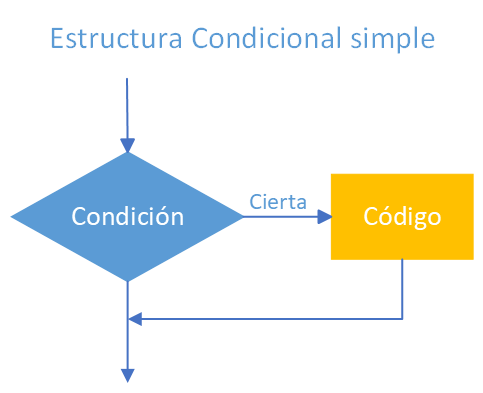
\includegraphics{./img/04-estructuras-control/condicional-simple.png}

}

\caption{Diagrama de flujo de la estructura condicional simple}

\end{figure}

\begin{figure}

{\centering 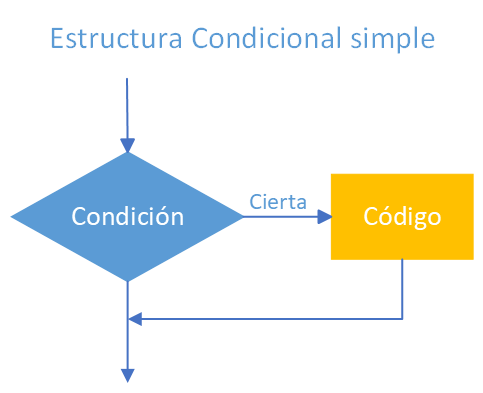
\includegraphics[width=0.7\textwidth,height=\textheight]{./img/04-estructuras-control/condicional-simple.png}

}

\caption{Diagrama de flujo de la estructura condicional simple}

\end{figure}

\leavevmode\vadjust pre{\hypertarget{exm-condicional-simple}{}}%
\begin{example}[]\label{exm-condicional-simple}

A continuación se muestra un ejemplo de estructura condicional con
\texttt{if}.

\begin{Shaded}
\begin{Highlighting}[]
\NormalTok{x }\OtherTok{\textless{}{-}} \DecValTok{1}
\NormalTok{y }\OtherTok{\textless{}{-}} \DecValTok{0}
\ControlFlowTok{if}\NormalTok{ (y }\SpecialCharTok{!=} \DecValTok{0}\NormalTok{)\{}
  \FunctionTok{print}\NormalTok{(x }\SpecialCharTok{/}\NormalTok{ y)}
\NormalTok{\}}
\end{Highlighting}
\end{Shaded}

\end{example}

Si se desea ejecutar un bloque de código alternativo cuando no se cumpla
la condición se puede añadir a continuación con la palabra reservada
\texttt{else}.

\begin{quote}
\texttt{if\ (}\emph{\texttt{\textless{}exp\textgreater{}}}\texttt{)\ \{}\strut \\
  \emph{\texttt{\textless{}código\ 1\textgreater{}}}\\
\texttt{\}\ else\ \{}\strut \\
  \emph{\texttt{\textless{}código\ 2\textgreater{}}}\\
\texttt{\}}
\end{quote}

En este caso, si la evaluación de la condición es \texttt{TRUE} se
ejecuta el código \texttt{\textless{}código\ 1\textgreater{}} y si es
\texttt{FALSE} se ejecuta el código
\texttt{\textless{}código\ 2\textgreater{}}.

\begin{figure}

{\centering 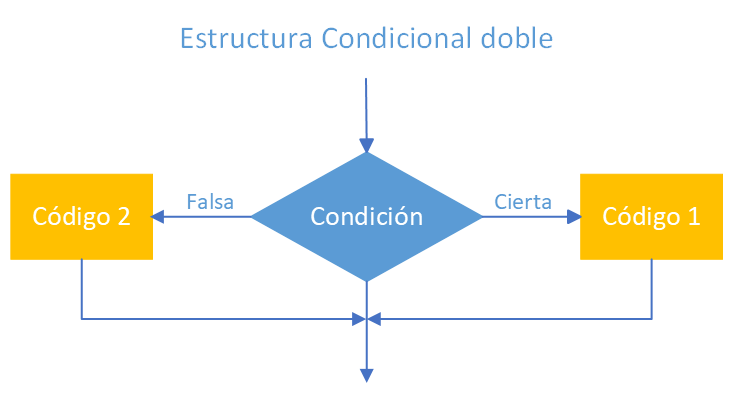
\includegraphics{./img/04-estructuras-control/condicional-doble.png}

}

\caption{Diagrama de flujo de la estructura condicional doble}

\end{figure}

\leavevmode\vadjust pre{\hypertarget{exm-condicional-doble}{}}%
\begin{example}[]\label{exm-condicional-doble}

A continuación se muestra un ejemplo de estructura condicional con
\texttt{if} y \texttt{else}.

\begin{Shaded}
\begin{Highlighting}[]
\NormalTok{nota }\OtherTok{\textless{}{-}} \FloatTok{8.5}
\ControlFlowTok{if}\NormalTok{ (nota }\SpecialCharTok{\textless{}} \DecValTok{5}\NormalTok{)\{}
  \FunctionTok{print}\NormalTok{(}\StringTok{"Suspenso"}\NormalTok{)}
\NormalTok{\} }\ControlFlowTok{else}\NormalTok{ \{}
  \FunctionTok{print}\NormalTok{(}\StringTok{"Aprobado"}\NormalTok{)}
\NormalTok{\}}
\end{Highlighting}
\end{Shaded}

\begin{verbatim}
[1] "Aprobado"
\end{verbatim}

\end{example}

Se puede comprobar más de una condición encadenando otra instrucción
\texttt{if} tras las instrucción \texttt{else}.

\begin{quote}
\texttt{if\ (}\emph{\texttt{\textless{}exp\ 1\textgreater{}}}\texttt{)\ \{}\strut \\
  \emph{\texttt{\textless{}código\ 1\textgreater{}}}\\
\texttt{\}\ else\ if\ (}\emph{\texttt{\textless{}exp\ 2\textgreater{}}}\texttt{)\ \{}\strut \\
  \emph{\texttt{\textless{}código\ 2\textgreater{}}}\texttt{)\ \{}\\
\ldots{}\\
\texttt{\}\ else\ \{}\strut \\
  \emph{\texttt{\textless{}código\ n\textgreater{}}}\\
\texttt{\}}
\end{quote}

Cuando se encadenan múltiples condiciones de esta forma, solamente se
ejecuta el bloque de código asociado a la primera condición cuya
evaluación sea \texttt{TRUE}. El último bloque de código solamente se
ejecuta si todas las condiciones son falsas.

\begin{figure}

{\centering 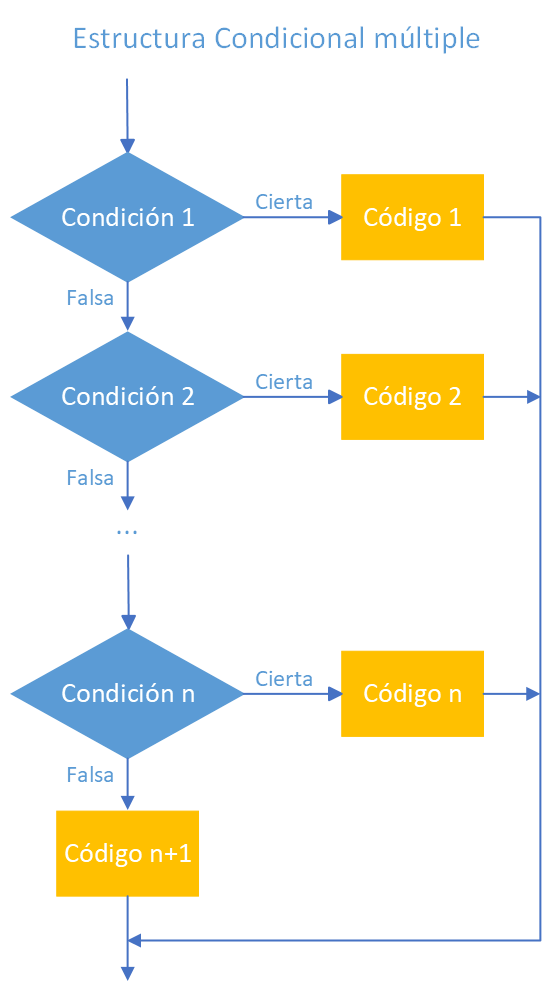
\includegraphics{./img/04-estructuras-control/condicional-multiple.png}

}

\caption{Diagrama de flujo de la estructura condicional múltiple}

\end{figure}

\leavevmode\vadjust pre{\hypertarget{exm-condicional-multiple}{}}%
\begin{example}[]\label{exm-condicional-multiple}

A continuación se muestra un ejemplo de estructura condicional múltiple.

\begin{Shaded}
\begin{Highlighting}[]
\NormalTok{nota }\OtherTok{\textless{}{-}} \FloatTok{8.5}
\ControlFlowTok{if}\NormalTok{ (nota }\SpecialCharTok{\textless{}} \DecValTok{5}\NormalTok{)\{}
  \FunctionTok{print}\NormalTok{(}\StringTok{"Suspenso"}\NormalTok{)}
\NormalTok{\} }\ControlFlowTok{else} \ControlFlowTok{if}\NormalTok{ (nota }\SpecialCharTok{\textless{}} \DecValTok{7}\NormalTok{) \{}
  \FunctionTok{print}\NormalTok{(}\StringTok{"Aprobado"}\NormalTok{)}
\NormalTok{\} }\ControlFlowTok{else} \ControlFlowTok{if}\NormalTok{ (nota }\SpecialCharTok{\textless{}} \DecValTok{9}\NormalTok{) \{}
  \FunctionTok{print}\NormalTok{(}\StringTok{"Notable"}\NormalTok{)}
\NormalTok{\} }\ControlFlowTok{else}\NormalTok{ \{}
  \FunctionTok{print}\NormalTok{(}\StringTok{"Sobresaliente"}\NormalTok{)}
\NormalTok{\}}
\end{Highlighting}
\end{Shaded}

\begin{verbatim}
[1] "Notable"
\end{verbatim}

\end{example}

\hypertarget{la-funciuxf3n-switch}{%
\subsection{\texorpdfstring{La función
\texttt{switch()}}{La función switch()}}\label{la-funciuxf3n-switch}}

Otra forma de tomar decisiones sobre el código a ejecutar es la función
\texttt{switch}.

\begin{itemize}
\tightlist
\item
  \texttt{switch(x,\ l)}: Ejecuta el código del valor de la lista
  \texttt{l} cuyo nombre asociado coincide con el resultado de evaluar
  la expresión \texttt{x}. Si el resultado de evaluar \texttt{x} no es
  ningún nombre de los elementos de la lista devuelve \texttt{NULL}.
\end{itemize}

\leavevmode\vadjust pre{\hypertarget{exm-condicional-switch}{}}%
\begin{example}[]\label{exm-condicional-switch}

A continuación se muestra un ejemplo de uso de la función
\texttt{switch}.

\begin{Shaded}
\begin{Highlighting}[]
\NormalTok{tipo.iva }\OtherTok{\textless{}{-}} \StringTok{"reducido"}
\NormalTok{precio }\OtherTok{\textless{}{-}} \DecValTok{1000}
\NormalTok{iva }\OtherTok{\textless{}{-}}\NormalTok{ precio }\SpecialCharTok{*} \ControlFlowTok{switch}\NormalTok{(tipo.iva, }\StringTok{"superreducido"} \OtherTok{=} \DecValTok{4}\NormalTok{, }\StringTok{"reducido"} \OtherTok{=} \DecValTok{10}\NormalTok{, }\StringTok{"normal"} \OtherTok{=} \DecValTok{21}\NormalTok{) }\SpecialCharTok{/} \DecValTok{100}
\NormalTok{iva}
\end{Highlighting}
\end{Shaded}

\begin{verbatim}
[1] 100
\end{verbatim}

\end{example}

\hypertarget{bucles}{%
\section{Bucles}\label{bucles}}

Un bucle es una estructura que permite la repetición de un bloque de
código. En R existen dos tipos de bucles, los \emph{bucles iterativos} y
los \emph{bucles condicionales}.

\hypertarget{bucles-iterativos-for}{%
\subsection{\texorpdfstring{Bucles iterativos
(\texttt{for})}{Bucles iterativos (for)}}\label{bucles-iterativos-for}}

Lo bucles iterativos repiten un bloque de código un número determinado
de veces. Comienzan por la palabra reservada \texttt{for} y llevan
asociado un \emph{iterador}, que es una variable que recorre una
secuencia de un tipo de datos compuesto, normalmente un vector o una
lista. El bloque de código se ejecuta tantas veces como elementos tenga
la secuencia, y en cada repetición el iterador toma como valor un
elemento distinto de la secuencia.

\begin{quote}
\texttt{for\ (}\emph{\texttt{i}}\texttt{in}\emph{\texttt{\textless{}secuencia\textgreater{}}}\texttt{)\ \{}\strut \\
  \emph{\texttt{\textless{}código\textgreater{}}}\\
\texttt{\}}
\end{quote}

\begin{figure}

{\centering 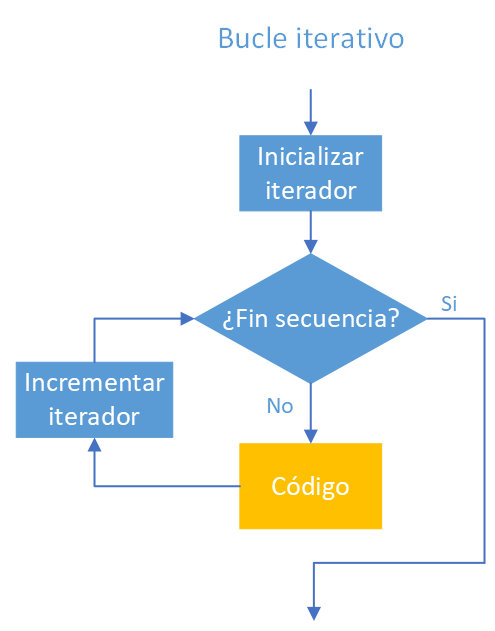
\includegraphics{./img/04-estructuras-control/bucle-for.png}

}

\caption{Diagrama de flujo de un bucle iterativo}

\end{figure}

\leavevmode\vadjust pre{\hypertarget{exm-bucle-iterarivo}{}}%
\begin{example}[]\label{exm-bucle-iterarivo}

A continuación se muestra varios ejemplos de uso del bucle \texttt{for}.

\begin{Shaded}
\begin{Highlighting}[]
\NormalTok{asignaturas }\OtherTok{\textless{}{-}} \FunctionTok{c}\NormalTok{(}\StringTok{"Matemáticas"}\NormalTok{, }\StringTok{"Física"}\NormalTok{, }\StringTok{"Programación"}\NormalTok{)}
\ControlFlowTok{for}\NormalTok{ (i }\ControlFlowTok{in}\NormalTok{ asignaturas) \{}
  \FunctionTok{print}\NormalTok{(i)}
\NormalTok{\}}
\end{Highlighting}
\end{Shaded}

\begin{verbatim}
[1] "Matemáticas"
[1] "Física"
[1] "Programación"
\end{verbatim}

\begin{Shaded}
\begin{Highlighting}[]
\ControlFlowTok{for}\NormalTok{ (i }\ControlFlowTok{in} \DecValTok{1}\SpecialCharTok{:}\DecValTok{5}\NormalTok{) \{}
  \FunctionTok{print}\NormalTok{(}\FunctionTok{paste}\NormalTok{(}\StringTok{"El cuadrado de "}\NormalTok{, i, }\StringTok{" es "}\NormalTok{, i}\SpecialCharTok{\^{}}\DecValTok{2}\NormalTok{))}
\NormalTok{\}}
\end{Highlighting}
\end{Shaded}

\begin{verbatim}
[1] "El cuadrado de  1  es  1"
[1] "El cuadrado de  2  es  4"
[1] "El cuadrado de  3  es  9"
[1] "El cuadrado de  4  es  16"
[1] "El cuadrado de  5  es  25"
\end{verbatim}

\end{example}

También es posible recorrer los elementos de la secuencia por posición
ayudándonos de la siguiente función:

\begin{itemize}
\tightlist
\item
  \texttt{seq\_along(x)}: que devuelve un vector con los enteros desde 1
  hasta el número de elementos de la secuencia \texttt{x}.
\end{itemize}

\leavevmode\vadjust pre{\hypertarget{exm-bucle-iterativo-posicion}{}}%
\begin{example}[]\label{exm-bucle-iterativo-posicion}

A continuación se muestra un ejemplo de bucle \texttt{for} que recorre
los elementos de un vector por posición.

\begin{Shaded}
\begin{Highlighting}[]
\NormalTok{asignaturas }\OtherTok{\textless{}{-}} \FunctionTok{c}\NormalTok{(}\StringTok{"Matemáticas"}\NormalTok{, }\StringTok{"Física"}\NormalTok{, }\StringTok{"Programación"}\NormalTok{)}
\ControlFlowTok{for}\NormalTok{ (i }\ControlFlowTok{in} \FunctionTok{seq\_along}\NormalTok{(asignaturas))\{}
  \FunctionTok{print}\NormalTok{(}\FunctionTok{paste}\NormalTok{(}\StringTok{"Asignatura "}\NormalTok{, i, }\StringTok{":"}\NormalTok{, asignaturas[i]))}
\NormalTok{\}}
\end{Highlighting}
\end{Shaded}

\begin{verbatim}
[1] "Asignatura  1 : Matemáticas"
[1] "Asignatura  2 : Física"
[1] "Asignatura  3 : Programación"
\end{verbatim}

\end{example}

Los bucles iterativos se utilizan habitualmente para recorrer
estructuras de una dimensión como los vectores y las listas, donde se
sabe de antemano el número de elementos que contiene y, por tanto, el
número de iteraciones del bucle. No obstante, también se pueden recorrer
estructuras de más de una dimensión, como por ejemplo matrices,
utilizando varios bucles \texttt{for} anidados.

\leavevmode\vadjust pre{\hypertarget{exm-bucles-anidados}{}}%
\begin{example}[]\label{exm-bucles-anidados}

A continuación se muestra varios ejemplos de dos bucles \texttt{for}
anidados para recorrer los elementos de una matriz.

\begin{Shaded}
\begin{Highlighting}[]
\NormalTok{x }\OtherTok{\textless{}{-}} \FunctionTok{matrix}\NormalTok{(}\DecValTok{1}\SpecialCharTok{:}\DecValTok{6}\NormalTok{, }\DecValTok{2}\NormalTok{, }\DecValTok{3}\NormalTok{)}
\ControlFlowTok{for}\NormalTok{ (i }\ControlFlowTok{in} \DecValTok{1}\SpecialCharTok{:}\FunctionTok{nrow}\NormalTok{(x)) \{}
  \ControlFlowTok{for}\NormalTok{ (j }\ControlFlowTok{in} \DecValTok{1}\SpecialCharTok{:}\FunctionTok{ncol}\NormalTok{(x))\{}
    \FunctionTok{print}\NormalTok{(x[i,j])}
\NormalTok{  \}}
\NormalTok{\}}
\end{Highlighting}
\end{Shaded}

\begin{verbatim}
[1] 1
[1] 3
[1] 5
[1] 2
[1] 4
[1] 6
\end{verbatim}

\end{example}

\hypertarget{bucles-condicionales-while}{%
\subsection{\texorpdfstring{Bucles condicionales
(\texttt{while})}{Bucles condicionales (while)}}\label{bucles-condicionales-while}}

Los bucles condicionales repiten un bloque de código mientras se cumpla
una condición. Comienzan con la palabra reservada \texttt{while} y
llevan asociada una expresión lógica, de manera que mientras la
evaluación de la expresión lógica sea \texttt{TRUE} se repite la
ejecución del bloque de código que contiene.

\begin{quote}
\texttt{while\ (}\emph{\texttt{\textless{}condición\textgreater{}}}\texttt{)\ \{}\strut \\
  \emph{\texttt{\textless{}código\textgreater{}}}\\
\texttt{\}}
\end{quote}

La expresión lógica \texttt{\textless{}condición\textgreater{}} se
evalúa antes de ejecutar el bloque de código y solo se ejecuta el
\texttt{\textless{}código\textgreater{}} si el resultado de la
evaluación es \texttt{TRUE}. Obsérvese que cuando el flujo de ejecución
del programa llega al bucle \texttt{while} si la condición no es cierta,
el código no se ejecuta ni tan siquiera una vez.

\begin{figure}

{\centering 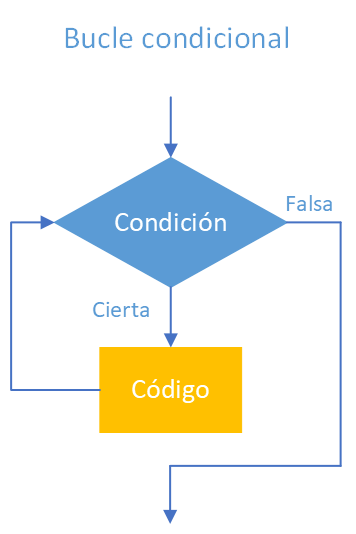
\includegraphics{./img/04-estructuras-control/bucle-while.png}

}

\caption{Diagrama de flujo de un bucle condicional}

\end{figure}

\leavevmode\vadjust pre{\hypertarget{exm-bucle-condicional}{}}%
\begin{example}[]\label{exm-bucle-condicional}

A continuación se muestra un ejemplo de bucle \texttt{while}.

\begin{Shaded}
\begin{Highlighting}[]
\NormalTok{i }\OtherTok{\textless{}{-}} \DecValTok{5}
\ControlFlowTok{while}\NormalTok{ (i }\SpecialCharTok{\textgreater{}=} \DecValTok{0}\NormalTok{) \{}
  \FunctionTok{print}\NormalTok{(i)}
\NormalTok{  i }\OtherTok{\textless{}{-}}\NormalTok{ i }\SpecialCharTok{{-}} \DecValTok{1}
\NormalTok{\}}
\end{Highlighting}
\end{Shaded}

\begin{verbatim}
[1] 5
[1] 4
[1] 3
[1] 2
[1] 1
[1] 0
\end{verbatim}

\end{example}

\hypertarget{la-instrucciuxf3n-break}{%
\subsection{\texorpdfstring{La instrucción
\texttt{break}}{La instrucción break}}\label{la-instrucciuxf3n-break}}

La instrucción \texttt{break} se utiliza para detener un bucle y salir
de él, tanto en bucles iterativos como en bucles condicionales.
Normalmente se suele utilizar esta instrucción cuando se cumple una
determinada condición en bloque de código del bucle y se decide parar su
ejecución y salir del bucle.

\leavevmode\vadjust pre{\hypertarget{exm-salida-bucle-break}{}}%
\begin{example}[]\label{exm-salida-bucle-break}

A continuación se muestra un ejemplo de uso de la instrucción
\texttt{break}.

\begin{Shaded}
\begin{Highlighting}[]
\CommentTok{\# Bucle que recorre los números enteros del {-}2 al 2 pero termina al llegar al 0.}
\ControlFlowTok{for}\NormalTok{ (i }\ControlFlowTok{in} \SpecialCharTok{{-}}\DecValTok{2}\SpecialCharTok{:}\DecValTok{2}\NormalTok{) \{}
  \ControlFlowTok{if}\NormalTok{ (i }\SpecialCharTok{==} \DecValTok{0}\NormalTok{) \{}
    \ControlFlowTok{break}
\NormalTok{  \} }
  \FunctionTok{print}\NormalTok{(i)}
\NormalTok{\}}
\end{Highlighting}
\end{Shaded}

\begin{verbatim}
[1] -2
[1] -1
\end{verbatim}

\end{example}

\hypertarget{la-instrucciuxf3n-next}{%
\subsection{\texorpdfstring{La instrucción
\texttt{next}}{La instrucción next}}\label{la-instrucciuxf3n-next}}

La instrucción \texttt{next} se utiliza para interrumpir la ejecución
del bloque de código de un bucle, pero en lugar de salir del bucle pasa
a la siguiente iteración. Si se trata de un bucle iterativo el iterador
pasa al siguiente elemento de la secuencia de iteración y si se trata de
un bucle condicional se pasa evaluar de nuevo la condición de
repetición.

:::\{\#exm-continuacion-bucle-next\} A continuación se muestra un
ejemplo de uso de la instrucción \texttt{next}.

\begin{Shaded}
\begin{Highlighting}[]
\CommentTok{\# Bucle que recorre los enteros del 1 al 10 pero solo imprime los números pares.}
\ControlFlowTok{for}\NormalTok{ (i }\ControlFlowTok{in} \DecValTok{1}\SpecialCharTok{:}\DecValTok{10}\NormalTok{) \{}
  \ControlFlowTok{if}\NormalTok{ (i }\SpecialCharTok{\%\%} \DecValTok{2}\NormalTok{) \{}
    \ControlFlowTok{next}
\NormalTok{  \}}
  \FunctionTok{print}\NormalTok{(i)}
\NormalTok{\}}
\end{Highlighting}
\end{Shaded}

\begin{verbatim}
[1] 2
[1] 4
[1] 6
[1] 8
[1] 10
\end{verbatim}

\bookmarksetup{startatroot}

\hypertarget{funciones}{%
\chapter{Funciones}\label{funciones}}

Una función es un bloque de código que tiene asociado un nombre, de
manera que cada vez que se quiera ejecutar el bloque de código basta con
invocar el nombre de la función. Las funciones permite dividir el código
en unidades lógicas que resultan más fáciles de manejar y mantener.

En R las funciones son objetos en sí mimas y pueden usarse como
cualquier otro dato. El tipo de dato de las funciones es
\texttt{function}.

\hypertarget{definiciuxf3n-y-llamada-a-funciones}{%
\section{Definición y llamada a
funciones}\label{definiciuxf3n-y-llamada-a-funciones}}

Para definir una función se utiliza la siguiente estructura de código:

\begin{quote}
\emph{\texttt{nombre.funcion}}
\texttt{\textless{}-\ function\ (}\emph{\texttt{parámetros}}\texttt{)\ \{}
  \emph{\texttt{\textless{}código\textgreater{}}}\\
\texttt{\}}
\end{quote}

El código que va entre llaves se conoce como \emph{cuerpo de la
función}.

Para llamar a la función y que se ejecute el código de su cuerpo hay que
utilizar el nombre de la función y a continuación los valores pasados a
sus parámetros entre paréntesis.

\leavevmode\vadjust pre{\hypertarget{exm-creacion-funcion}{}}%
\begin{example}[]\label{exm-creacion-funcion}

A continuación se muestra un ejemplo de creación y llamada a una
función.

\begin{Shaded}
\begin{Highlighting}[]
\CommentTok{\# Definición de la función}
\NormalTok{saludo }\OtherTok{\textless{}{-}} \ControlFlowTok{function}\NormalTok{() \{}
  \FunctionTok{print}\NormalTok{(}\StringTok{"¡Hola!"}\NormalTok{)}
\NormalTok{\}}
\FunctionTok{class}\NormalTok{(saludo)}
\end{Highlighting}
\end{Shaded}

\begin{verbatim}
[1] "function"
\end{verbatim}

\begin{Shaded}
\begin{Highlighting}[]
\CommentTok{\# Llamada a la función}
\FunctionTok{saludo}\NormalTok{()}
\end{Highlighting}
\end{Shaded}

\begin{verbatim}
[1] "¡Hola!"
\end{verbatim}

\end{example}

\hypertarget{paruxe1metros-y-argumentos-de-una-funciuxf3n}{%
\section{Parámetros y argumentos de una
función}\label{paruxe1metros-y-argumentos-de-una-funciuxf3n}}

Una función puede recibir valores cuando se invoca a través de unas
variables conocidas como \emph{parámetros} que se definen entre
paréntesis en la declaración de la función. En el cuerpo de la función
se pueden usar estos parámetros como si fuesen variables.

Los valores que se pasan a la función en una llamada o invocación
concreta de ella se conocen como \emph{argumentos} y se asocian a los
parámetros de la declaración de la función.

\leavevmode\vadjust pre{\hypertarget{exm-funcion-con-parametros}{}}%
\begin{example}[]\label{exm-funcion-con-parametros}

A continuación se muestra un ejemplo de una función con parámetros.

\begin{Shaded}
\begin{Highlighting}[]
\CommentTok{\# Función con un parámetro}
\NormalTok{saludo }\OtherTok{\textless{}{-}} \ControlFlowTok{function}\NormalTok{(nombre) \{}
  \FunctionTok{print}\NormalTok{(}\FunctionTok{paste}\NormalTok{(}\StringTok{"¡Hola "}\NormalTok{, nombre, }\StringTok{"!"}\NormalTok{, }\AttributeTok{sep =} \StringTok{""}\NormalTok{))}
\NormalTok{\}}
\CommentTok{\# Llamada a la función con un argumento}
\FunctionTok{saludo}\NormalTok{(}\StringTok{"Alf"}\NormalTok{)}
\end{Highlighting}
\end{Shaded}

\begin{verbatim}
[1] "¡Hola Alf!"
\end{verbatim}

En este ejemplo la función \texttt{saludo} tiene un parámetro
\texttt{nombre}. En la llamada a la función se pasa la cadena
\texttt{Alf} como argumento que se asocia al parámetro \texttt{nombre}
en el cuerpo de la función.

\end{example}

\hypertarget{paso-de-argumentos-a-una-funciuxf3n}{%
\subsection{Paso de argumentos a una
función}\label{paso-de-argumentos-a-una-funciuxf3n}}

Los argumentos de una función pueden pasarse de dos formas:

\begin{itemize}
\tightlist
\item
  \textbf{Argumentos posicionales}: Se asocian a los parámetros de la
  función en el mismo orden que aparecen en la definición de la función.
\item
  \textbf{Argumentos nominales}: Se indica explícitamente el nombre del
  parámetro al que se asocia un argumento de la forma
  \texttt{parametro\ =\ argumento}. En este caso el orden de los
  argumentos no importa.
\end{itemize}

\leavevmode\vadjust pre{\hypertarget{exm-paso-parametros-funcion}{}}%
\begin{example}[]\label{exm-paso-parametros-funcion}

A continuación se muestran varios ejemplos de pasos de argumentos
posicionales y nominales.

\begin{Shaded}
\begin{Highlighting}[]
\CommentTok{\# Función con un argumento por defecto}
\NormalTok{area.triangulo }\OtherTok{\textless{}{-}} \ControlFlowTok{function}\NormalTok{(base, altura) \{}
\NormalTok{  base }\SpecialCharTok{*}\NormalTok{ altura }\SpecialCharTok{/} \DecValTok{2}
\NormalTok{\}}
\CommentTok{\# Cálculo del área de un triángulo de base 4 y altura 3}
\CommentTok{\# Paso de argumentos por posición. }
\FunctionTok{area.triangulo}\NormalTok{(}\DecValTok{4}\NormalTok{, }\DecValTok{3}\NormalTok{)}
\end{Highlighting}
\end{Shaded}

\begin{verbatim}
[1] 6
\end{verbatim}

\begin{Shaded}
\begin{Highlighting}[]
\CommentTok{\# Paso de argumentos por nombre}
\FunctionTok{area.triangulo}\NormalTok{(}\AttributeTok{altura =} \DecValTok{3}\NormalTok{, }\AttributeTok{base =} \DecValTok{4}\NormalTok{)}
\end{Highlighting}
\end{Shaded}

\begin{verbatim}
[1] 6
\end{verbatim}

\end{example}

\hypertarget{argumentos-por-defecto}{%
\subsection{Argumentos por defecto}\label{argumentos-por-defecto}}

En la definición de una función se puede asignar a cada parámetro un
argumento por defecto, de manera que si se invoca la función sin
proporcionar ningún argumento para ese parámetro, se utiliza el
argumento por defecto.

\leavevmode\vadjust pre{\hypertarget{exm-argumento-defecto-funcion}{}}%
\begin{example}[]\label{exm-argumento-defecto-funcion}

A continuación se muestra un ejemplo de definición de una función con un
argumento por defecto.

\begin{Shaded}
\begin{Highlighting}[]
\NormalTok{saludo }\OtherTok{\textless{}{-}} \ControlFlowTok{function}\NormalTok{(nombre, }\AttributeTok{lenguaje =} \StringTok{"R"}\NormalTok{) \{}
  \FunctionTok{print}\NormalTok{(}\FunctionTok{paste}\NormalTok{(}\StringTok{"¡Hola "}\NormalTok{, nombre, }\StringTok{"! ¡Bienvenido a "}\NormalTok{, lenguaje, }\StringTok{"!"}\NormalTok{, }\AttributeTok{sep =} \StringTok{""}\NormalTok{))}
\NormalTok{\}}
\CommentTok{\# Llamada a la función con un argumento}
\FunctionTok{saludo}\NormalTok{(}\StringTok{"Alf"}\NormalTok{)}
\end{Highlighting}
\end{Shaded}

\begin{verbatim}
[1] "¡Hola Alf! ¡Bienvenido a R!"
\end{verbatim}

\end{example}

\hypertarget{retorno-de-una-funciuxf3n}{%
\section{Retorno de una función}\label{retorno-de-una-funciuxf3n}}

Una función puede devolver un objeto de cualquier tipo tras su
invocación. Para ello se utiliza la función \texttt{return()}, indicando
entre paréntesis el valor que devuelve la función. El retorno suele
realizarse al final del cuerpo de la función, porque con él finaliza la
ejecución de la función y se devuelve el control de la ejecución al
punto desde donde se llamó a la función, de manera que cualquier
instrucción de cuerpo que vaya después no se ejecutará. Si no se indica
ningún objeto, la función devolverá el valor de la última expresión
calculada en el cuerpo de la función.

\leavevmode\vadjust pre{\hypertarget{exm-retorno-funciones}{}}%
\begin{example}[]\label{exm-retorno-funciones}

A continuación se muestran varios ejemplos de retornos de funciones.

\begin{Shaded}
\begin{Highlighting}[]
\CommentTok{\# Función que devuelve el area de un triángulo}
\NormalTok{area.triangulo }\OtherTok{\textless{}{-}} \ControlFlowTok{function}\NormalTok{(base, altura) \{}
  \FunctionTok{return}\NormalTok{(base }\SpecialCharTok{*}\NormalTok{ altura }\SpecialCharTok{/} \DecValTok{2}\NormalTok{)}
\NormalTok{\}}
\FunctionTok{area.triangulo}\NormalTok{(}\DecValTok{4}\NormalTok{, }\DecValTok{3}\NormalTok{)}
\end{Highlighting}
\end{Shaded}

\begin{verbatim}
[1] 6
\end{verbatim}

\begin{Shaded}
\begin{Highlighting}[]
\CommentTok{\# Función que devuelve el valor absoluto de un número}
\NormalTok{valor.absoluto }\OtherTok{\textless{}{-}} \ControlFlowTok{function}\NormalTok{(x) \{}
  \ControlFlowTok{if}\NormalTok{ (x }\SpecialCharTok{\textless{}} \DecValTok{0}\NormalTok{)}
    \FunctionTok{return}\NormalTok{(x }\SpecialCharTok{*} \SpecialCharTok{{-}}\DecValTok{1}\NormalTok{)}
  \ControlFlowTok{else}
    \FunctionTok{return}\NormalTok{(x)}
\NormalTok{\}}
\FunctionTok{valor.absoluto}\NormalTok{(}\SpecialCharTok{{-}}\DecValTok{1}\NormalTok{)}
\end{Highlighting}
\end{Shaded}

\begin{verbatim}
[1] 1
\end{verbatim}

\begin{Shaded}
\begin{Highlighting}[]
\FunctionTok{valor.absoluto}\NormalTok{(}\DecValTok{2}\NormalTok{)}
\end{Highlighting}
\end{Shaded}

\begin{verbatim}
[1] 2
\end{verbatim}

\end{example}

Para devolver más de un valor se pueden utilizar estructuras de datos
como vectores, listas, matrices o data frames.

\leavevmode\vadjust pre{\hypertarget{exm-retorno-funcion-lista}{}}%
\begin{example}[]\label{exm-retorno-funcion-lista}

A continuación se muestra un ejemplo de una función de devuelve una
lista.

\begin{Shaded}
\begin{Highlighting}[]
\NormalTok{circulo }\OtherTok{\textless{}{-}} \ControlFlowTok{function}\NormalTok{(radio) \{}
  \FunctionTok{return}\NormalTok{(}\FunctionTok{list}\NormalTok{(}\AttributeTok{perimetro =} \DecValTok{2} \SpecialCharTok{*}\NormalTok{ pi }\SpecialCharTok{*}\NormalTok{ radio, }\AttributeTok{area =}\NormalTok{ pi }\SpecialCharTok{*}\NormalTok{ radio }\SpecialCharTok{\^{}} \DecValTok{2}\NormalTok{))}
\NormalTok{\}}
\FunctionTok{circulo}\NormalTok{(}\DecValTok{5}\NormalTok{)}
\end{Highlighting}
\end{Shaded}

\begin{verbatim}
$perimetro
[1] 31.41593

$area
[1] 78.53982
\end{verbatim}

\begin{Shaded}
\begin{Highlighting}[]
\FunctionTok{circulo}\NormalTok{(}\DecValTok{5}\NormalTok{)}\SpecialCharTok{$}\NormalTok{perimetro}
\end{Highlighting}
\end{Shaded}

\begin{verbatim}
[1] 31.41593
\end{verbatim}

\begin{Shaded}
\begin{Highlighting}[]
\FunctionTok{circulo}\NormalTok{(}\DecValTok{5}\NormalTok{)}\SpecialCharTok{$}\NormalTok{area}
\end{Highlighting}
\end{Shaded}

\begin{verbatim}
[1] 78.53982
\end{verbatim}

\end{example}

\hypertarget{entorno-y-uxe1mbito-de-las-variables}{%
\section{Entorno y ámbito de las
variables}\label{entorno-y-uxe1mbito-de-las-variables}}

El entorno de un programa en R es el conjunto de todos los objetos
(funciones, variables, etc.) creados durante la ejecución del programa.
Cuando se ejecuta el interprete de R siempre se crea un primer entorno
\texttt{R\_GlobalEnv} conocido como entorno global. Es posible referirse
a él en cualquier momento con la constante \texttt{.GlobalEnv}.

Para ver el entorno activo en cada momento de la ejecución y el
contenido del mismo se utiliza la siguiente función:

\begin{itemize}
\tightlist
\item
  \texttt{environment()}: Devuelve el nombre del entorno actual.
\item
  \texttt{ls()}: Devuelve un vector con los nombres de las objetos
  (variables, funciones, etc.) que contiene el entorno global.
\end{itemize}

\leavevmode\vadjust pre{\hypertarget{exm-acceso-entorno-global}{}}%
\begin{example}[]\label{exm-acceso-entorno-global}

A continuación se muestra un ejemplo acceso al entorno global de un
programa.

\begin{Shaded}
\begin{Highlighting}[]
\NormalTok{x }\OtherTok{\textless{}{-}} \DecValTok{4}
\NormalTok{y }\OtherTok{\textless{}{-}} \DecValTok{3}
\NormalTok{area.triangulo }\OtherTok{\textless{}{-}} \ControlFlowTok{function}\NormalTok{(base, altura) \{}
\NormalTok{  base }\SpecialCharTok{*}\NormalTok{ altura }\SpecialCharTok{/} \DecValTok{2}
\NormalTok{\}}
\FunctionTok{environment}\NormalTok{()}
\end{Highlighting}
\end{Shaded}

\begin{verbatim}
<environment: R_GlobalEnv>
\end{verbatim}

\begin{Shaded}
\begin{Highlighting}[]
\FunctionTok{ls}\NormalTok{()}
\end{Highlighting}
\end{Shaded}

\begin{verbatim}
[1] "area.triangulo" "x"              "y"             
\end{verbatim}

\end{example}

Como se puede observar en el ejemplo anterior, los parámetros de la
función \texttt{base} y \texttt{altura} no aparecen en el entorno
global. En R, cuando se ejecuta una función se crea un nuevo entorno
hijo dentro del entorno al que pertenece la función. Durante la
ejecución de la función este pasa a ser el entorno activo y cuando
termina la ejecución de la función deja de serlo y vuelve a activarse el
entorno padre desde donde se llamó a la función.

\leavevmode\vadjust pre{\hypertarget{exm-activacion-entorno-funcion}{}}%
\begin{example}[]\label{exm-activacion-entorno-funcion}

A continuación se muestra un ejemplo de activación del entorno de una
función.

\begin{Shaded}
\begin{Highlighting}[]
\NormalTok{x }\OtherTok{\textless{}{-}} \DecValTok{4}
\NormalTok{y }\OtherTok{\textless{}{-}} \DecValTok{3}
\NormalTok{area.triangulo }\OtherTok{\textless{}{-}} \ControlFlowTok{function}\NormalTok{(base, altura) \{}
  \FunctionTok{print}\NormalTok{(}\StringTok{"Entorno de la función area.triangulo"}\NormalTok{) }
  \FunctionTok{print}\NormalTok{(}\FunctionTok{environment}\NormalTok{())}
  \FunctionTok{print}\NormalTok{(}\FunctionTok{ls}\NormalTok{())}
  \FunctionTok{return}\NormalTok{(base }\SpecialCharTok{*}\NormalTok{ altura }\SpecialCharTok{/} \DecValTok{2}\NormalTok{)}
\NormalTok{\}}
\FunctionTok{print}\NormalTok{(}\StringTok{"Entorno fuera de la función"}\NormalTok{)}
\end{Highlighting}
\end{Shaded}

\begin{verbatim}
[1] "Entorno fuera de la función"
\end{verbatim}

\begin{Shaded}
\begin{Highlighting}[]
\FunctionTok{environment}\NormalTok{()}
\end{Highlighting}
\end{Shaded}

\begin{verbatim}
<environment: R_GlobalEnv>
\end{verbatim}

\begin{Shaded}
\begin{Highlighting}[]
\FunctionTok{ls}\NormalTok{()}
\end{Highlighting}
\end{Shaded}

\begin{verbatim}
[1] "area.triangulo" "x"              "y"             
\end{verbatim}

\begin{Shaded}
\begin{Highlighting}[]
\FunctionTok{area.triangulo}\NormalTok{(x, y)}
\end{Highlighting}
\end{Shaded}

\begin{verbatim}
[1] "Entorno de la función area.triangulo"
<environment: 0x561b2928d8d0>
[1] "altura" "base"  
\end{verbatim}

\begin{verbatim}
[1] 6
\end{verbatim}

\end{example}

Los parámetros y los objetos (funciones, variables, etc.) definidos
dentro de una función son de \emph{ámbito local}, mientras que los
objetos definidos fuera de ella en alguno de los entornos ancestros son
de \emph{ámbito global}.

Tanto los parámetros como las variables del ámbito local de una función
sólo están accesibles durante la ejecución de la función, es decir,
cuando termina la ejecución de la función estas variables desaparecen y
no son accesibles desde fuera de la función.

Cuando una función declara un objeto (función, variable, etc.) que ya
existe en alguno de los entornos ancestros con ámbito global, durante la
ejecución de la función el objeto global queda eclipsado por el local y
no es accesible hasta que finaliza la ejecución de la función.

\leavevmode\vadjust pre{\hypertarget{exm-eclise-variables-globales-por-locales}{}}%
\begin{example}[]\label{exm-eclise-variables-globales-por-locales}

A continuación se muestra un ejemplo de eclipse de una variable de
ámbito global por otra de ámbito local.

\begin{Shaded}
\begin{Highlighting}[]
\NormalTok{lenguaje }\OtherTok{=} \StringTok{"Python"}
\NormalTok{saludo }\OtherTok{\textless{}{-}} \ControlFlowTok{function}\NormalTok{(lenguaje) \{}
  \FunctionTok{print}\NormalTok{(}\FunctionTok{paste}\NormalTok{(}\StringTok{"Bienvenido a"}\NormalTok{, lenguaje))  }
\NormalTok{\}}
\FunctionTok{saludo}\NormalTok{(}\StringTok{"R"}\NormalTok{)}
\end{Highlighting}
\end{Shaded}

\begin{verbatim}
[1] "Bienvenido a R"
\end{verbatim}

Obsérvese cómo al ejecutar la función anterior, la variable
\texttt{lenguaje} queda inaccesible al tener la función un parámetro con
el mismo nombre.

\end{example}

Las variables globales están accesibles siempre que no sean eclipsadas
por otras con el mismo nombre de ámbito local. Si embargo, cuando se
intenta asignar un valor a una variable global en el ámbito local, se
crea una nueva variable local. Para asignar valores a variables globales
en el ámbito local se tiene que utilizar el operador de superasignación
\texttt{\textless{}\textless{}-}. Cuando se utiliza este operador para
asignar un valor a una variable, R busca la variable entorno padre, y si
no existe continua con la búsqueda en los entornos ancestros hasta
llegar a entorno global. Si la búsqueda tiene éxito, asigna el nuevo
valor a la variable global, mientras que si no tiene éxito se crea una
nueva variable de ámbito local y se le asigna el valor.

\leavevmode\vadjust pre{\hypertarget{exm-superasignacion}{}}%
\begin{example}[]\label{exm-superasignacion}

A continuación se muestra un ejemplo del uso del operador de
superasignación.

\begin{Shaded}
\begin{Highlighting}[]
\NormalTok{saludo }\OtherTok{\textless{}{-}} \ControlFlowTok{function}\NormalTok{() \{}
\NormalTok{  lenguaje }\OtherTok{\textless{}\textless{}{-}} \StringTok{"R"}
  \FunctionTok{return}\NormalTok{(}\FunctionTok{paste}\NormalTok{(}\StringTok{"Bienvenido a"}\NormalTok{, lenguaje))}
\NormalTok{\}}
\NormalTok{lenguaje}
\end{Highlighting}
\end{Shaded}

\begin{verbatim}
[1] "Python"
\end{verbatim}

\end{example}

\hypertarget{componentes-de-una-funciuxf3n}{%
\section{Componentes de una
función}\label{componentes-de-una-funciuxf3n}}

Los tres componentes de una función son:

\begin{itemize}
\tightlist
\item
  \textbf{Cuerpo}: Es el código dentro de la función.
\item
  \textbf{Parámetros}: Es la lista de parámetros que requiere la
  función.
\item
  \textbf{Entorno}: Es donde se ubican las variables de la función.
\end{itemize}

Para acceder a estos componentes se pueden utilizar las siguientes
funciones:

\begin{itemize}
\tightlist
\item
  \texttt{body(f)}: Devuelve el cuerpo de la función \texttt{f}.
\item
  \texttt{formals(f)}: Devuelve la lista de parámetros de la función
  \texttt{f}.
\item
  \texttt{environment(f)}: Devuelve el entorno de la función \texttt{f}.
\end{itemize}

\leavevmode\vadjust pre{\hypertarget{exm-componentes-funcion}{}}%
\begin{example}[]\label{exm-componentes-funcion}

A continuación se muestra un ejemplo de acceso a los componentes de una
función.

\begin{Shaded}
\begin{Highlighting}[]
\CommentTok{\# Definición de la función}
\NormalTok{area.triangulo }\OtherTok{\textless{}{-}} \ControlFlowTok{function}\NormalTok{(base, altura) \{}
\NormalTok{  base }\SpecialCharTok{*}\NormalTok{ altura }\SpecialCharTok{/} \DecValTok{2}
\NormalTok{\}}
\FunctionTok{body}\NormalTok{(area.triangulo)}
\end{Highlighting}
\end{Shaded}

\begin{verbatim}
{
    base * altura/2
}
\end{verbatim}

\begin{Shaded}
\begin{Highlighting}[]
\FunctionTok{formals}\NormalTok{(area.triangulo)}
\end{Highlighting}
\end{Shaded}

\begin{verbatim}
$base


$altura
\end{verbatim}

\begin{Shaded}
\begin{Highlighting}[]
\FunctionTok{environment}\NormalTok{(saludo)}
\end{Highlighting}
\end{Shaded}

\begin{verbatim}
<environment: R_GlobalEnv>
\end{verbatim}

\end{example}

\hypertarget{funciones-recursivas}{%
\section{Funciones recursivas}\label{funciones-recursivas}}

Una función recursiva es una función que en su cuerpo contiene una llama
a sí misma.

La recursión es una práctica común en la mayoría de los lenguajes de
programación ya que permite resolver las tareas recursivas de manera más
natural.

Para garantizar el final de una función recursiva, las sucesivas
llamadas tienen que reducir el grado de complejidad del problema, hasta
que este pueda resolverse directamente sin necesidad de volver a llamar
a la función. De lo contrario la recursión no tendría fin y nunca
terminaría la ejecución de la función.

\leavevmode\vadjust pre{\hypertarget{exm-funcion-recursiva}{}}%
\begin{example}[]\label{exm-funcion-recursiva}

A continuación se muestra un ejemplo de una función recursiva.

\begin{Shaded}
\begin{Highlighting}[]
\NormalTok{factorial }\OtherTok{\textless{}{-}} \ControlFlowTok{function}\NormalTok{(n) \{}
  \ControlFlowTok{if}\NormalTok{ (n }\SpecialCharTok{\textless{}=} \DecValTok{1}\NormalTok{) }\FunctionTok{return}\NormalTok{(n)}
  \ControlFlowTok{else} \FunctionTok{return}\NormalTok{(n }\SpecialCharTok{*} \FunctionTok{factorial}\NormalTok{(n }\SpecialCharTok{{-}} \DecValTok{1}\NormalTok{))}
\NormalTok{\}}
\FunctionTok{factorial}\NormalTok{(}\DecValTok{4}\NormalTok{)}
\end{Highlighting}
\end{Shaded}

\begin{verbatim}
[1] 24
\end{verbatim}

\end{example}

\hypertarget{paquetes}{%
\section{Paquetes}\label{paquetes}}

Para facilitar la reutilización código y datos R permite la creación de
paquetes que pueden importarse desde otros programas. Un paquete es una
colección de código, funciones y datos que se almacenan en un fichero
dentro de un directorio llamado \texttt{library} en el entorno de R.
Para ver la ubicación de este directorio dentro del sistema de archivos
local se puede utilizar la función \texttt{.libPaths()}.

\leavevmode\vadjust pre{\hypertarget{exm-ubiacion-biblioteca-paquetes}{}}%
\begin{example}[]\label{exm-ubiacion-biblioteca-paquetes}

A continuación se muestra un ejemplo de la ubicación del directorio
\texttt{library}.

\begin{Shaded}
\begin{Highlighting}[]
\FunctionTok{.libPaths}\NormalTok{()}
\end{Highlighting}
\end{Shaded}

\begin{verbatim}
[1] "/home/alf/R/x86_64-pc-linux-gnu-library/4.2"
[2] "/usr/lib/R/library"                         
\end{verbatim}

\end{example}

Durante la instalación de R también se instalan varios paquetes básicos
que están disponibles en cualquier sesión de trabajo con R. Pero añadir
nuevas funciones o procedimientos es necesario instalar el paquete que
los contiene y después cargarlo en la sesión de trabajo.

Para ver los paquetes instalados en un ordenador se utiliza la función
\texttt{library()}.

\hypertarget{instalaciuxf3n-de-paquetes}{%
\subsection{Instalación de paquetes}\label{instalaciuxf3n-de-paquetes}}

La mayor parte de los paquetes para R están disponibles en el
repositorio oficial
\href{Comprehensive\%20R\%20Archive\%20Network}{CRAN} (Comprehensive R
Archive Network), aunque cualquier persona puede desarrollar un paquete
y ponerlo a disposición de la comunidad en cualquier otro repositorio.

Existen distintas formas de instalar un paquete en R:

\begin{itemize}
\tightlist
\item
  Directamente desde el repositorio oficial CRAN
\item
  Desde otros repositorios no oficiales (por ejemplo Github)
\item
  Descargando el paquete e instalándolo manualmente.
\end{itemize}

\hypertarget{instalaciuxf3n-de-paquetes-desde-el-repositorio-cran}{%
\subsubsection{Instalación de paquetes desde el repositorio
CRAN}\label{instalaciuxf3n-de-paquetes-desde-el-repositorio-cran}}

Para instalar un paquete desde el repositorio oficial CRAN se utiliza la
siguiente función:

\begin{itemize}
\tightlist
\item
  \texttt{install.packages(x)}: Obtiene el paquete con el nombre
  \texttt{x} desde un servidor con el repositorio CRAN y lo instala
  localmente en el directorio \texttt{library} del entorno de R. Se
  puede instalar más de un paquete a la vez pasando un vector con los
  nombres de los paquetes.
\end{itemize}

\leavevmode\vadjust pre{\hypertarget{exm-instalacion-paquetes}{}}%
\begin{example}[]\label{exm-instalacion-paquetes}

A continuación se muestra un ejemplo de instalación de paquetes desde el
repositorio CRAN.

\begin{Shaded}
\begin{Highlighting}[]
\FunctionTok{install.packages}\NormalTok{(}\StringTok{"devtools"}\NormalTok{)}
\end{Highlighting}
\end{Shaded}

\end{example}

\hypertarget{instalaciuxf3n-desde-otros-repositorios-github-gitlab-etc.}{%
\subsubsection{Instalación desde otros repositorios (GitHub, GitLab,
etc.)}\label{instalaciuxf3n-desde-otros-repositorios-github-gitlab-etc.}}

El paquete \texttt{remotes} incorpora funciones para instalar paquetes
alojados en otros repositorios habituales para el desarrollo de software
como \href{https://github.com/}{GitHub},
\href{httpsb://gitlab.com/}{GitLab} o
\href{https://www.bioconductor.org/}{Bioconductor}.

\leavevmode\vadjust pre{\hypertarget{exm-instalacion-paquetes-github}{}}%
\begin{example}[]\label{exm-instalacion-paquetes-github}

A continuación se muestra un ejemplo de instalación de paquetes desde
GitHub.

\begin{Shaded}
\begin{Highlighting}[]
\FunctionTok{install.packages}\NormalTok{(}\StringTok{"remotes"}\NormalTok{)}
\NormalTok{remotes}\SpecialCharTok{::}\FunctionTok{install\_github}\NormalTok{(}\StringTok{"rkward{-}community/rk.Teaching"}\NormalTok{)}
\end{Highlighting}
\end{Shaded}

\end{example}

\hypertarget{instalaciuxf3n-manual}{%
\subsubsection{Instalación manual}\label{instalaciuxf3n-manual}}

Finalmente es posible instalar un paquete manualmente a partir de su
código fuente. Para ello hay previamente hay que descargar el código
fuente del paquete en un fichero comprimido en formato zip y después
utilizar la siguiente función:

\begin{itemize}
\tightlist
\item
  \texttt{install.packages(x,\ repos\ =\ NULL,\ type\ =\ "source")}:
  Instala el paquete ubicado en la ruta \texttt{x} del sistema de
  archivos local en la librería \texttt{library}.
\end{itemize}

Una vez instalado un paquete ya está disponible para cargarlo en
cualquier sesión de trabajo de R y no es necesario volver a instalarlo.

\hypertarget{carga-de-un-paquete}{%
\subsection{Carga de un paquete}\label{carga-de-un-paquete}}

Una vez instalado un paquete, para poder ejecutar su contenido es
necesario cargarlo en el entorno de trabajo de R. Para ello se utiliza
la siguiente función:

\begin{itemize}
\tightlist
\item
  \texttt{library(x)}: Ejecuta el código del paquete \texttt{x} en la
  sesión de trabajo activa.
\end{itemize}

\leavevmode\vadjust pre{\hypertarget{exm-carga-paquetes}{}}%
\begin{example}[]\label{exm-carga-paquetes}

A continuación se muestra un ejemplo de carga de un paquete.

\begin{Shaded}
\begin{Highlighting}[]
\FunctionTok{library}\NormalTok{(}\StringTok{"remotes"}\NormalTok{)}
\end{Highlighting}
\end{Shaded}

\end{example}

\hypertarget{paquetes-habituales}{%
\subsection{Paquetes habituales}\label{paquetes-habituales}}

A continuación se presenta una lista ordenada alfabéticamente (no por
importancia) de los paquetes más populares para el análisis de datos:

\begin{itemize}
\tightlist
\item
  \href{https://topepo.github.io/caret/index.html}{\texttt{caret}} es un
  paquete para la creación de modelos de clasificación y regresión
  mediante aprendizaje automático.
\item
  \href{https://www.rdocumentation.org/packages/data.table/}{\texttt{data.table}}
  es un paquete para la manipulación de grandes conjuntos de datos (de
  hasta 100GB) de manera rápida y eficiente.
\item
  \href{https://www.rdocumentation.org/packages/devtools/}{\texttt{devtools}}
  es un paquete con herramientas para el desarrollo de paquetes en R.
\item
  \href{https://www.r-project.org/nosvn/pandoc/knitr.html}{\texttt{knitr}}
  es un paquete que proporciona un motor para la generación de informes
  dinámicos que permite la integración de código en R con los lenguajes
  de procesamiento de textos LaTeX, HTML, Markdown, AsciiDoc o
  reStructuredText.
\item
  \href{https://mlr3.mlr-org.com/}{\texttt{mlr3}} es un paquete que
  proporciona funciones para las principales técnicas de aprendizaje
  automático.
\item
  \href{https://plotly.com/r/}{\texttt{plotly}} es un paquete para la
  creación de gráficos interactivos.
\item
  \href{https://rmarkdown.rstudio.com/}{\texttt{rmarkdown}} es un
  paquete que facilita el uso del paquete \texttt{knitr} para la
  elaboración de documentos en múltiples formatos (HTML, pdf, Word y
  otros) permitiendo la integración de código R en el lenguaje Markdown.
\item
  \href{https://shiny.rstudio.com/}{\texttt{shiny}} es un paquete para
  la construcción de aplicaciones web interactivas.
\item
  \href{https://www.tidymodels.org/}{\texttt{tidymodels}} es una
  colección de paquetes para la construcción y evalucación de modelos
  con técnicas de aprendizaje automático.
\item
  \href{https://www.tidyverse.org/}{\texttt{tidyverse}} es una colección
  de paquetes para la Ciencia de Datos que incluye paquetes para la
  carga, limpieza, manipulación y representación gráfica de datos.
\end{itemize}



\end{document}
